
%%%%%%%%%%%%%%%%%%%%%%%%%%%%%%%%%%%%%%%%%%%%%%%%%%%%%%%%%%%%%%%%%%%%
%                               PREAMBLE
%%%%%%%%%%%%%%%%%%%%%%%%%%%%%%%%%%%%%%%%%%%%%%%%%%%%%%%%%%%%%%%%%%%%

\documentclass[a4paper, 10pt, twoside, openright]{report}
\usepackage[top = 120pt, left = 100pt, right = 100pt, bottom = 100pt]{geometry}
\usepackage[french]{babel}
\usepackage[utf8]{inputenc} 
\usepackage[T1]{fontenc}
\usepackage[sc]{mathpazo}
\linespread{1.05}         % Palladio needs more leading (space between lines)
\usepackage[hidelinks]{hyperref}
\usepackage{ulem}
\usepackage{fancyhdr}
\usepackage{shorttoc}

\usepackage{xcolor}
\usepackage{pagecolor}
\usepackage{graphicx}
\usepackage{tikz}
\usepackage{epigraph}
\usepackage{fancyhdr}
\usepackage{blkarray}
\usepackage{booktabs}
\usepackage{eso-pic}
\usepackage{picture}
%\usepackage{svg}

\usepackage{amsfonts}
\usepackage{amsmath}
\usepackage{amsthm}
\usepackage{stmaryrd}
\usepackage{multicol}
\usepackage{bbold}
\usepackage{amssymb}
\usepackage{yhmath}
\usepackage{xfrac}
\usepackage{dsfont}
\usepackage{mathrsfs}
\usepackage{cancel}
\usepackage{soul}

\usepackage{shorttoc}
\usepackage{minitoc}

% \renewcommand{\thefootnote}{\fnsymbol{footnote}}


\pagestyle{fancy}
\setlength{\headheight}{13.59999pt}
\fancyhead[LE]{\thepage}
\fancyhead[RE]{\small \leftmark}
\fancyhead[LO]{\small \rightmark}
\fancyhead[RO]{\thepage}
\fancyfoot[C]{}


\makeatletter
\renewcommand\part{%
  \if@openright
    \clearpage{\thispagestyle{empty}\cleardoublepage}
  \else
    \clearpage
  \fi
  \thispagestyle{empty}%
  \if@twocolumn
    \onecolumn
    \@tempswatrue
  \else
    \@tempswafalse
  \fi
  \null\vfil
  \secdef\@part\@spart}

\renewcommand\chapter{\if@openright\clearpage{\thispagestyle{empty}\cleardoublepage}\else\clearpage\fi
                    \thispagestyle{empty}%
                    \global\@topnum\z@
                    \@afterindentfalse
                    \secdef\@chapter\@schapter}


\makeatother


%%%%%%%%%%%%%%%%%%%%%%%%%%%%%%%%%%%%%%%%%%%%%%%%%%%%%%%%%%%%%%%%%%%%
%                            Cover Page Details
%%%%%%%%%%%%%%%%%%%%%%%%%%%%%%%%%%%%%%%%%%%%%%%%%%%%%%%%%%%%%%%%%%%%

\renewcommand\epigraphflush{flushright}
\renewcommand\epigraphsize{\normalsize}
\setlength\epigraphwidth{0.7\textwidth}

\definecolor{titlepagecolor}{cmyk}{0.6,0.6,0.6,0.4}

\DeclareFixedFont{\titlefont}{T1}{ppl}{b}{it}{0.5in}

\makeatletter                       
\def\printauthor{%                  
    {\large \@author}}              
\makeatother
\author{%
    Mis en forme par \\
    Émile Sauvat \\
    \texttt{emile.sauvat@ens.psl.eu}\vspace{20pt}}

% The following code is borrowed from: https://tex.stackexchange.com/a/86310/10898

\newcommand\titlepagedecoration{%
\begin{tikzpicture}[remember picture,overlay,shorten >= -10pt]

\coordinate (aux1) at ([yshift=-15pt]current page.north east);
\coordinate (aux2) at ([yshift=-410pt]current page.north east);
\coordinate (aux3) at ([xshift=-4.5cm]current page.north east);
\coordinate (aux4) at ([yshift=-150pt]current page.north east);

\begin{scope}[titlepagecolor!40,line width=12pt,rounded corners=12pt]
\draw
  (aux1) -- coordinate (a)
  ++(225:5) --
  ++(-45:5.1) coordinate (b);
\draw[shorten <= -10pt]
  (aux3) --
  (a) --
  (aux1);
\draw[opacity=0.6,titlepagecolor,shorten <= -10pt]
  (b) --
  ++(225:2.2) --
  ++(-45:2.2);
\end{scope}
\draw[titlepagecolor,line width=8pt,rounded corners=8pt,shorten <= -10pt]
  (aux4) --
  ++(225:0.8) --
  ++(-45:0.8);
\begin{scope}[titlepagecolor!70,line width=6pt,rounded corners=8pt]
\draw[shorten <= -10pt]
  (aux2) --
  ++(225:3) coordinate[pos=0.45] (c) --
  ++(-45:3.1);
\draw
  (aux2) --
  (c) --
  ++(135:2.5) --
  ++(45:2.5) --
  ++(-45:2.5) coordinate[pos=0.3] (d);   
\draw 
  (d) -- +(45:1);
\end{scope}
\end{tikzpicture}%
}

\begin{document}


%%%%%%%%%%%%%%%%%%%%%%%%%%%%%%%%%%%%%%%%%%%%%%%%%%%%%%%%%%%%%%%%%%%%
%                            Command Definitions
%%%%%%%%%%%%%%%%%%%%%%%%%%%%%%%%%%%%%%%%%%%%%%%%%%%%%%%%%%%%%%%%%%%%

\newcommand{\dessin}[2]{
    \begin{center}
        \input{dessins/#1}
        \captionof{figure}{#2}
    \end{center}    }


%%%    Some command to create theorem and definition easier      %%%

\theoremstyle{plain}
\newtheorem{thm}{Théorème}[section]
\newtheorem{lem}[thm]{Lemme}
\newtheorem{prop}[thm]{Proposition}
\newtheorem*{cor}{Corollaire}
\newcommand{\theorem}[2]{
    \hspace{15pt}
    	\begin{minipage}[t]{\textwidth}
    	\begin{#1} ~\vspace{1pt} \\
			\hspace*{15pt} {\vrule width 1pt} \kern2pt
    		\begin{minipage}[t]{0.7\textwidth}	
                #2 
     		\end{minipage}
     	\end{#1}
     	\end{minipage}
     \medskip
    }
    %commande pour créer un théorème, le premier argument est le type et le second le contenu
        % ex : \theorem{lem}{contenu du lemme}
    
\newcommand{\namedtheorem}[3]{
    \newtheorem*{#3}{#1}
    \hspace{15pt}
    	\begin{minipage}[t]{\textwidth}
    	\begin{#3} ~\vspace{1pt} \\
			\hspace*{15pt} {\vrule width 1pt} \kern2pt
    		\begin{minipage}[t]{0.7\textwidth}	
                #2 
     		\end{minipage}
     	\end{#3}
     	\end{minipage}
    }

\theoremstyle{remark}
\newtheorem*{nd}{Note}
\newcommand{\remarque}[1]{\begin{nd} #1 \medskip \end{nd}}
    %commande pour créer une remarque, le contenu passe en argument
        % ex : \remarque{contenu de la remarque}
\newtheorem*{rap}{Rappel}
\newcommand{\rappel}[1]{\begin{rap} #1 \medskip \end{rap}}

\newcommand{\traitd}{\begin{center} ~ \medskip  \\ \rule{0.9\textwidth}{0.75pt} \vspace{-10pt}\end{center}}
\newcommand{\trait}{\vspace{-5pt} \begin{center} \rule{0.9\textwidth}{0.75pt} \end{center} ~ }
\newcommand{\traitdouble}{\trait \vspace{-30pt} \traitd}

\makeatletter
\newcommand*{\ar}{\@ifstar\ard\arf}
\makeatother
\newcommand{\ard}{\begin{array}{l}}
\newcommand{\arf}{\end{array}}


%%%     Maths misc      %%%

\newcommand{\abs}[1]{\left\vert #1 \right\vert}

\newcommand{\appli}[4]{
    \left(
    \begin{array}{ccc} 
        #1 & \longrightarrow & #3 \\ 
        #2 & \longmapsto & #4
    \end{array}
    \right)
}


\newcommand{\ent}[1]{{\llbracket #1 \rrbracket}}                    
	% Ensemble d'entiers
\newcommand{\N}{{\mathbb{N}}}                                       
	% Entiers naturels
\newcommand{\Z}{{\mathbb{Z}}}                                       
	% Entiers relatifs
\newcommand{\R}{{\mathbb{R}}}                                       
	% Réels
\newcommand{\C}{{\mathbb{C}}}                                       
	% Complexes
\newcommand{\K}{{\mathbb{K}}}                                       
	% Corps K
\newcommand{\Q}{{\mathbb{Q}}}                                       
	% Rationnels
\newcommand{\KX}{{\mathbb{K}[X]}}                                   
	% Polynômes sur K
\newcommand{\M}{{\mathcal{M}}}                                      
	% Matrices
\newcommand{\GL}{{\mathcal{G}\hspace*{-0.05cm} \mathcal{L}}}        
	% Groupe Linéaire
\newcommand{\cont}{{\mathcal{C}}}                                   
	% Fonctions continues
\newcommand{\Cinf}{\mathscr{C}^{\infty}}
    % Fonctions C infini
\newcommand{\cpm}{{\mathcal{C}_{pm}^0}}                             
	% Fonctions continues par morceaux
\newcommand{\lin}{{\mathcal{L}}}                                    
	% Applications linéaires
\newcommand{\Sym}{{\mathcal{S}}}                                    
	% Matrices symétrique
\newcommand{\Orth}{{\mathcal{O}}}                                   
	% Matrices orthogonales
\newcommand{\bigo}{{\mathcal{O}}}
    % Dommination
\newcommand{\Part}{\mathcal{P}}                                     
	% Parties
\newcommand{\A}{{\mathscr{A}}}                                      
	% Tribu
\newcommand{\Esc}{{\mathcal{E}\big([a,b],\R\big)}}
    % Fonction en escalier
\newcommand{\prehilb}{(E,\scal{.,.})}
    % Espacee préhilbertien
\newcommand{\Img}{\mathrm{im}}
	% Image d'une application


\newcommand{\norm}[1]{\left\Vert #1 \right\Vert}
    % Norme
\newcommand{\normop}[1]{{\left\vert\kern-0.15ex\left\vert\kern-0.15ex\left\vert #1 \right\vert\kern-0.15ex\right\vert\kern-0.15ex\right\vert}} 
    % Norme subordonnée
\newcommand{\scal}[1]{\left< #1 \right>}
    % Produit scalaire


\newcommand{\suminf}{\sum_{n=0}^\infty}
    % Somme infinie en n
\newcommand{\sk}[2]{\sum_{k= #1 }^{#2}}
    % Somme en k
\newcommand{\si}[2]{\sum_{i= #1 }^{#2}}
    % Somme en i
\newcommand{\pk}[2]{\prod\_{k= #1 }^{#2}}
    % Produit en k
\newcommand{\pdi}[2]{\prod_{i= #1 }^{#2}}
    % Produit en i
\newcommand{\se}{\sum_{n\geq 0} a_nz^n}

\newcommand{\Ps}{\sum_{k=0}^{+\infty} a_k X^k}
    % Polynôme infini
\newcommand{\Psn}{\sum_{k=0}^n a_k X^k}
    % Polynôme degré n

\newcommand{\sumi}{\sum\limits_{i\in I}}
    % Somme sur un ensemble I
\newcommand{\prodi}{\prod\limits_{i\in I}}
    % Produit sur un ensemble I


\newcommand{\suite}[1]{(#1_n)}
    % Suite en n
\newcommand{\stox}[1]{\underset{x \to #1}{\longrightarrow}}
    % Convergence selon x
\newcommand{\ston}{\underset{n}{\rightarrow}}
    % Convergence en n
\newcommand{\limit}[2]{{\underset{#1 \rightarrow #2}{\lim}}}
    % Limite


\newcommand{\pfrac}[2]{\frac{\partial #1}{\partial #2}}
    % Dérivée partielle


%%%     Format      %%%

\newcommand{\highlight}[1]{\colorbox{lightgray}{#1}}
    % Surligner en gris

\newcommand{\col}[2]{\begin{multicols}{2} #1 \columnbreak \\ #2 \end{multicols}}
    % Deux colonnes

\newcommand{\fin}{
	~ \vspace{10pt}\\
    \begin{center}
        { \LARGE $\star$ \hspace{0.7cm} $\star$ \hspace{0.7cm} $\star$ }
    \end{center}
    }


%%%%%%%%%%%%%%%%%%%%%%%%%%%%%%%%%%%%%%%%%%%%%%%%%%%%%%%%%%%%%%%%%%%%
%                               COVER
%%%%%%%%%%%%%%%%%%%%%%%%%%%%%%%%%%%%%%%%%%%%%%%%%%%%%%%%%%%%%%%%%%%%

\begin{titlepage}

\noindent
\titlefont ~\vspace{50pt}\\Mathématiques \\ \hspace*{150pt} Préparatoires II\par
\epigraph{\textsl{Les charmes enchanteurs de cette sublime science ne se décèlent dans toute leur beauté qu'à ceux qui ont le courage de l'approfondir}} %
{Carl Friedrich Gauss\\Quelques années plus tôt}
\null\vfill
\vspace*{1cm}
\noindent
\hfill
\begin{minipage}{0.45\linewidth}
    \begin{flushright}
        \printauthor
    \end{flushright}
\end{minipage}
%
\begin{minipage}{0.02\linewidth}
    \vspace{-20pt}
    \rule{1pt}{55pt}
\end{minipage}
\titlepagedecoration
\end{titlepage}

\setcounter{tocdepth}{2}
%\renewcommand{\thefootnote}{\fnsymbol{footnote}}
\renewcommand{\contentsname}{Table des matières - Deuxième année}
\setcounter{minitocdepth}{4}
\renewcommand{\mtctitle}{Contenu}
\dominitoc

\thispagestyle{empty}
\vspace*{100pt}

\begin{minipage}[t]{0.8\textwidth}

Ce document est une synthèse du cours de mathématiques dispensé par M. Jean-François Mallordy 
en classe préparatoire au lycée Blaise Pascal, Clermont-Ferrand en 2022-2023. Il s'agit d'un complément au cours de Maths Spé 
et ne saurait en aucun cas y être un quelconque remplacement ! \vspace{10pt}\\

\noindent Merci à Kellian pour les heures de discussion et pour sa relecture attentive. \\

\noindent Merci à mes professeurs Laurent Germa et Jean-François Mallordy pour leur enseignement et leur soutient.
	
\end{minipage}

\vfill

\begin{flushright}
	%\includesvg[width = 0.3\linewidth]{../../sig/signatureSVG}
	
\includegraphics[width = 0.4\textwidth]{../../sig/signature.jpg}
	\vskip 20pt
	\textit{
	Paris, 2024
	}
\end{flushright}

\vfill

\shorttoc{Chapitres}{0}
\thispagestyle{empty}
%
%\newpage
%
%\AddToShipoutPicture*{
%	\put(\linewidth/2 ,300)
%	{	
%		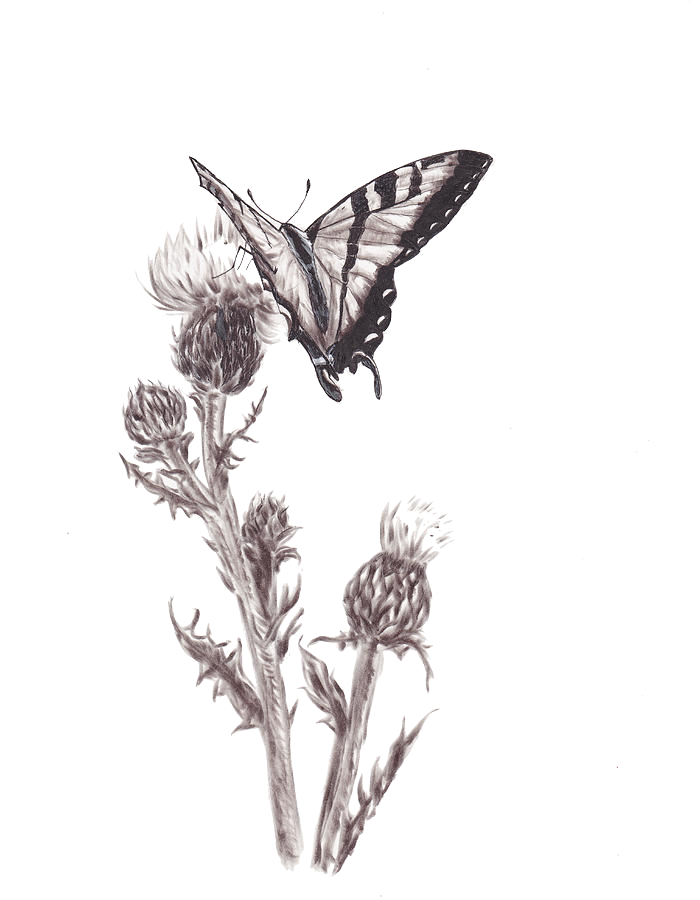
\includegraphics[width = 0.5\textwidth]{../../illustr/butterfly.png} 
%		
%	}
%}

\theoremstyle{plain}

%%%%%%%%%%%%%%%%%%%%%%%%%%%%%%%%%%%%%%%%%%%%%%%%%%%%%%%%%%%%%%%%%%%%
%                          DOCUMENT START
%%%%%%%%%%%%%%%%%%%%%%%%%%%%%%%%%%%%%%%%%%%%%%%%%%%%%%%%%%%%%%%%%%%%

%\setcounter{chapter}{21}

\chapter{Suites et séries}
	\thispagestyle{empty}

    
% Chapitre 1 : Suites et séries 

\textit{\small On considèrera comme acquis en sup les cas réel et complexe : Notament:\\ -> Théorème des gendarmes \hfill -> Théorème de la limite monotone} \hfill ${}$

% \minitoc

\section{Norme}

	\subsection{Généralités}
	
		\vspace{-15pt}
		\traitd
		\paragraph{Norme} Une \emph{norme} sur $E$ est une application $N: E \rightarrow\mathbf{R}$ vérifiant : 
			\begin{itemize}
				\item $\forall x\in E, ~N(x) = 0_{\mathbf{R}} ~\Leftrightarrow ~x=0_E$
				\item $\forall x\in E, ~\forall \lambda \in \mathbf{K} , ~N(\lambda .x) = \abs{\lambda}N(x)$
				\item $ \forall x,y \in E, ~N(x+y) \leq N(x)+N(y)$ 
			\end{itemize}
		\trait 
		
		\theorem{lem}{Soit $(E,N)$ un espace vectoriel normé, \\
			On a $N\geq 0$ \hspace*{1cm} {\small (i.e. $\forall x\in E,~N(x-y) \geq 0$)}
			}
			
		\traitd
		\paragraph{Distance} Une \emph{distance} sur $X$ est une application $d:X^2\rightarrow\mathbf{R}$ vérifiant:
			\begin{itemize}
				\item $\forall x,y\in E, ~d(x,y) = 0 ~\Leftrightarrow ~x=y$
				\item $\forall x,y\in E, ~d(x,y)~=~d(y,x)$
				\item $\forall x,y,z\in E, ~d(x,z)~\leq~d(x,y)+d(y,z)$
			\end{itemize}
		\trait
		
		\theorem{lem}{Soit $(E,N)$ un espace vectoriel normé. \\
			Si $\forall (x,y)\in E^2$, $d(x,y) = N(x-y) $ alors $d$ est une distance sur E.
			}
			
		\traitd
		\paragraph{Boule ouverte et fermée} Soient $a\in E,~r\in\mathbf{R}$ On pose
			\[B(a,r) = \left\{ x\in E ~|~ d(x,a)<r\right\} \hspace*{1.5cm} B_f (a,r) = \left\{ x\in E ~|~ d(x,a) \leq r\right\}\]
			\hspace*{0.6cm} Les \emph{boules ouverte et fermée} de centre $a$ et de rayon $r$. 
		\traitdouble
		\paragraph{Segment et ensemble convexe} Soit $E$ un $\mathbf{K}$ espace vectoriel quelconque \vspace*{0.2cm}\\
			\hspace*{0.5cm} -> Pour $(a,b)\in E^2$ on défini le \emph{segment} : $[a,b]=\left\{ (1-t)a +tb ~\vert ~t\in [0,1]\right\}$ \\
			\hspace*{0.5cm} -> $\mathcal{C} \subset E$ est dit \emph{convexe} si $\forall (a,b)\in \mathcal{C}^2,~[a,b]\subset \mathcal{C}$
		\trait 
		
		\theorem{lem}{Dans $E$ un EVN quelconque les boules sont convexes} \\

	\subsection{Normes euclidiennes}
		Ici $E$ est un $\mathbf{R}$ espace vectoriel muni d'un produit scalaire\footnotemark[1] 
		\[
			\Phi :  \appli{E^2}{(x,y)}{\mathbf{R}}{\scal{x}{y}}
		\]
			
		\footnotetext[1]{Un produit scalaire est une forme bilinéaire symétrique définie positive}
		
		On a alors par théorème\footnote[2]{Voir cours de sup} ,  $x\mapsto \sqrt{\scal{x}{x}}$ est une norme sur $E$.  
		On notera \begin{center} \highlight{ $\norm{x}_2 = N_2(x) = \sqrt{\scal{x}{x}}$ } \end{center} 
		
		\remarque{L'inégalité triangulaire pour $\norm{.}_2$ est dite inégalité de \emph{Minkovsky}} ~\\
			
		\theorem{lem}{Si $E=\mathbf{C}^n ,~z=\left(z_1,\dots ,z_n\right) ~, ~N(z) = \sqrt{\sum\limits_{k=1}^n\abs{z_k}^2}$ est une norme
			} \medskip \\
		
		\theorem{lem}{$E = \cont^0\left([a,b],\mathbf{C}\right)$ Soit $f\in E$ on pose \\
			$N(f) = \sqrt{\int_a^b \abs{f(x)}^2\mathrm{d}x}$ \hspace*{1cm} alors $N$ est une norme sur $E$
			}

		\medskip
			
	\subsection{Exemple de normes}

		\paragraph{Norme $N_{\infty}$ :}~
		
			Dans $E=K^n$ soit $x=(x_1,\dots ,x_n) ,~ N_{\infty}(x) = 
			\underset{i\in\ent{1,n}}{\mathrm{max}} \abs{x_i}$
		
			Dans $E=\cont^0([a,b],K)$ soit $f\in E,~N_{\infty} (f) = \underset{x\in [a,b]}{\mathrm{sup}} \abs{f(x)}$
			
		\paragraph{Norme $N_1$ :} ~

			Dans $E=K^n$ soit $x=(x_1,\dots ,x_n) ,~ N_1(x) = \sum_{i=1}^n \abs{x_i} $
			
			Dans $E=\cont^0([a,b],K)$ soit $f\in E,~N_1 (f) = \int_a^b \abs{f(x)} \mathrm{d}x$
			
		\paragraph{Norme $N_2$ :} ~

			Dans $E=K^n$ soit $x=(x_1,\dots ,x_n) ,~ N_2(x) = \sqrt{\sum_{i=1}^n x_i^{~2}} $
			
			Dans $E=\cont^0([a,b],K)$ soit $f\in E,~N_2 (f) = \sqrt{\int_a^b \left( f(x)\right)^2 \mathrm{d}x}$
		
		\medskip


\section{Suites}
		
		\vspace{-15pt}
		\traitd 
		\paragraph{Suite convergente}	
			Soit $u=\left( u_n\right)_{_{n\in\mathbf{N}}} \in E^{\mathbf{N}}$ et $\ell\in E$.
			On dit que $u$ converge vers $\ell$ et on note 
			\[
				u_n \underset{n\rightarrow +\infty}{\longrightarrow} \ell ~\mathrm{ssi}~\forall 
				\varepsilon >0 ,~\exists n_0 \in \mathbf{N} ~:~ \forall n\geq n_0,~d(u_n ,\ell) <\varepsilon
			\vspace{-15pt}
			\] 
		\trait 
			
		\namedtheorem{Lemme 1 : Unicité de la limite}{
			Si \hspace*{0.2cm}
			$\ard u_n \underset{n}{\rightarrow} \ell_1 ~\in E \\u_n \underset{n}{\rightarrow} \ell_2 ~\in E \arf$ \hspace*{0.2cm} Alors $\ell_1 = \ell_2$
			}{UniqLimit}
			
		\begin{proof}
			Par l'absurde, on suppose $\ell_1\neq \ell_2$.\\
			Soit $\varepsilon = \frac{1}{2} d(\ell_1,\ell_2) >0$
			On a alors $\ard n_1 \in \mathbf{N} ~:~\forall n\geq n_1 ,~d(u_n,\ell_1) < \varepsilon \\  
			n_2 \in \mathbf{N} ~:~\forall n\geq n_2 ,~d(u_n,\ell_2) < \varepsilon \arf $  et soit $p=max(n_1,n_2)$ \vspace*{0.1cm}\\
			$d(\ell_1,\ell_2) \leq d(\ell_1,u_p) + d(\ell_2,u_p) < 2\varepsilon = d(\ell_1,\ell_2)$  \emph{impossible}
		\end{proof} \medskip
		
		\theorem{lem}{
			Soit $\left(u_n\right) _{_{n\in \mathbf{N} }} \in E^{\mathbf{N}} ,~\ell\in E $\hspace*{0.2cm} 
			Alors $u_n \underset{n}{\rightarrow} \ell ~\Leftrightarrow ~\norm{u_n - \ell} \underset{n}{\rightarrow} 0$
		}
		
		\begin{proof}
			Notons $v_n = \norm{u_n-\ell}$ et $\lambda = 0$
			Alors $d(u_n,\ell) = \norm{u_n - \ell} = v_n = \norm{v_n - \lambda} = d(v_n,\lambda )$ \\
			or $u_n \underset{n}{\rightarrow} \ell$ \emph{ssi} : $\forall \varepsilon >0 ,~\exists n_0 \in \mathbf{N} ~:~ 
			\forall n\geq n_0,~d(u_n ,\ell) <\varepsilon ~\Rightarrow ~ d(v_n,\lambda)<\varepsilon ~\Rightarrow ~ v_n \underset{n}{\rightarrow} 0$
		\end{proof} \medskip

		\theorem{lem}{
			Soient $u_n ,~v_n \in E^{\mathbf{N}} ~$ et $ \lambda\in K$ si on a 
			$u_n \underset{n}{\rightarrow} \alpha$ et $v_n \underset{n}{\rightarrow} \beta$\\ 
			\hspace*{0.2cm} Alors $\lambda u_n + v_n \underset{n}{\rightarrow} \lambda\alpha + \beta$
		} \medskip \\

		\namedtheorem{Lemme : Inégalité triangulaire renversée}{
			Soit $x,y \in E$ alors $\abs{N(x) - N(y)} \leq N(x-y)$
		}{InegTriRenv}

		\begin{proof}
			$N(x)\leq N(x-y) + N(y) \Rightarrow ~ \underbrace{N(x) - N(y)}_{t\in \mathbf{R}} \leq N(x-y)$\\
			On conclut alors par agument de symétrie.
		\end{proof} \medskip

			
		\theorem{lem}{
			Soit $u_n \in E^{\mathbf{N}} ,~\alpha\in K$ 
			on a $u_n\underset{n}{\rightarrow} \alpha ~\Rightarrow ~ \norm{u_n}\underset{n}{\rightarrow}\norm{\alpha}$ 
		} \medskip \\ {\small \emph{Attention !} La réciproque est fausse !}

		\vspace{-15pt}
		\traitd
		\paragraph{Suite bornée}
			Soit $\left(u_n\right)_{n\in\mathbf{N}} \in E^{\mathbf{N}}$ on dit que $\left(u_n\right)$ est bornée si
			$\exists M \in \mathbf{R} ~:~ \forall n\in\mathbf{N} ,~\norm{u_n}\leq M$. 
		\trait

		\theorem{lem}{
			Toute suite $\left(u_n\right)_{n\geq 0} \in E^{\mathbf{N}}$ convergente est bornée
		} \medskip \\

		\theorem{lem}{
			On suppose $\left\{\ard \lambda_n \underset{n}{\rightarrow} \mu \in K \\ 
			u_n \underset{n}{\rightarrow} v\in E \arf\right.$ \hspace*{0.2cm} Alors $\lambda_n u_n \underset{n}{\rightarrow} \mu v$
		} 
		
		\newpage
		
		\traitd
		\paragraph{Suite extraite}
			Soit $u \in E^{\mathbf{N}}$ on appelle \emph{suite extraite} (ou sous-suite) de $u$ toute suite
			$\left(u_{\varphi (n)}\right)_{n\in \mathbf{N}}$ où $\varphi : \mathbf{N} \rightarrow \mathbf{N}$ 
			est une extractrice (injection croissante) \\ \textit{\small NB : en fait $\left(v_n\right)_{n\geq0} = 
			\left(u_{\varphi (n)} \right)_{n\geq 0} ~\Leftrightarrow ~v= u\circ\varphi$} 
		\traitdouble
		\paragraph{Valeur d'adhérence}
			$\ell\in E$ est une valeur d'adhérence de $u$ s'il existe une suite extraite de $u$ qui converge vers $\ell$.
			On notera $\mathcal{V}_u$ l'ensemble des valeurs d'adhérence de $u$. 
		\trait
		
		\theorem{thm}{
			Soit $u\in E^{\mathbf{N}}$ si $u$ \\
			converge vers $\ell\in K$ 
			alors toute suite extraite de $u$ converge vers $\ell$
		}
		
		\begin{proof}
			Soit $\varphi : \mathbf{N} \rightarrow \mathbf{N}$ une extractrice et 
			$\left(v_n\right)_{n\geq 0} = \left(u_{\varphi (n)} \right)_{n\geq 0}$ \\
			Soit $\varepsilon >0$ et $ n_0 \in\mathbf{N} ~:~ \forall n\geq n_0 ,~d(u_n ,\ell)<\varepsilon$ 
			donc $\varphi (n) \geq n_0$ et ainsi $d\left( u_{\varphi (n)},\ell\right)<\varepsilon$ et $v_n \underset{n}{\rightarrow} \ell$
		\end{proof} \medskip

		\theorem{cor}{
			Toute suite admettant au moins $2$ valeurs d'adhérence est \\divergente
		} 
		
		\medskip 

\section{Normes équivalentes}
	
	\subsection{Définition}
		
	\vspace{-10pt}
		\traitd \vspace{-7pt}~\\
			Soit $E$ un $K$ espace vectoriel, $N$ et $N'$ deux normes sur $E$.
			$N$ et $N'$ sont dites \\équivalentes ($N\sim N'$) si $\exists \alpha ,\beta \in \mathbf{R} ~:~ \alpha N \leq N'\leq \beta N$
		\trait

		\vspace{-10pt}
		\remarque{On peut aussi l'écrire $	N'\leq \beta N$ et $N\leq \frac{1}{\alpha} N'$\\} 
		
		\theorem{lem}{
			Soit $N,N'$ des normes équivalentes sur $E$, $u\in E^{\mathbf{N}} ,~\ell\in E$ alors\\
			1) $u_n \underset{n}{\rightarrow}\ell$ dans $(E,N)$ $\Leftrightarrow$ $u_n \underset{n}{\rightarrow}\ell$ dans $(E,N')$ \\
			2) $u$ est bornée dans $(E,N)$ $ \Leftrightarrow$ $u$ est bornée dans $(E,N')$
		}
		
		\theorem{lem}{
			Sur $K^n$, $N_1$, $N_2$ et $N_{\infty}$ sont équivalentes et plus précisément
			\\ \hspace*{2cm} $N_{\infty} \leq N_1 \leq \sqrt{n}N_2 \leq nN_{\infty}$
		} 
		
		\medskip

	\subsection{Cas de espaces de dimension fini}
		
		\rappel{Un espace vectoriel $E$ est de dimension finie s'il existe une famille d'éléments de $E$ 
			libre et génératrice, c'est alors une base de $E$.} \medskip
			
		\theorem{thm}{
			Sur un $K$-ev de dimension finie, 
			toutes les normes sont équivalentes.
		} \medskip \\
		\textit{\small Sera démontré ultérieurement.} \\

		\theorem{cor}{
			Dans un $K$ espace vectoriel de dimension finie, 
			la notion de convergence \\
			ne dépend pas de la norme.
		} \medskip \\ 
		\emph{Attention !} C'est faux en dimension quelconque ! \\

		\theorem{lem}{
			Soit $E$ de dimension finie et $e = (e_1,\dots ,e_p)$ une base de $E$. \\
			Soit $\left(x_n\right)_{n\geq 0} \in E^{\mathbf{N}}$ et $\alpha \in E$.
			On écrit $\left\{\ard x_n = x_{1,n}e_1 + \cdots + x_{p,n}e_p \\ \alpha = \alpha_1e_1 + \cdots + \alpha_pe_p \arf\right.$\\
			On a alors $x_n \underset{n}{\rightarrow} \alpha ~\Leftrightarrow ~\forall k \in \ent{1,p} ,~x_{k,n} \underset{n}{\rightarrow} \alpha_k$
		} \medskip \\
		
		\theorem{thm}{
			Soient $p,q,r \in \mathbf{N}^*$
			\hspace*{0.3cm}$\left\{\begin{array}{ll} A_n \underset{n}{\rightarrow} A & dans~\mathcal{M}_{p,q}\left(\mathbf{R}\right) \\ 
			B_n \underset{n}{\rightarrow} B & dans~\mathcal{M}_{q,r}\left(\mathbf{R}\right) \end{array}\right.$ \hspace*{0.3cm}
			Alors $A_nB_n \underset{n}{\rightarrow} AB$
		}
		
		\begin{proof}
			Soit $(i,j)\in\ent{1,p}\times\ent{1,r}$ \\ 
			$\left(A_nB_n\right) _{i,j} = \sum_{k=1}^{q} \underbrace{\left(A_n\right)_{i,k}}_{\rightarrow a_{i,k}}
			\underbrace{\left(B_n\right)_{k,j}}_{\rightarrow b_{k,j}}$ $\underset{n}{\rightarrow} \sum_{k=1}^{q} a_{i,k}b_{k,j} = (AB)_{i,j}$ donc 
			$A_nB_n \underset{n}{\rightarrow} AB$
		\end{proof}


\section{Comparaisons asymptotiques}
	
		Soient $\left(u_n\right)_{n\geq n_0} ,\left(v_n\right)_{n\geq n_0} \in \mathbf{C}^{\mathbf{N}}$ 
		
		\traitd
		\paragraph{Négligeabilité}
			On dit que $u_n$ est négligeable devant $v_n$ quand $n\rightarrow +\infty$ noté $u_n \underset{n\rightarrow +\infty}{=} \circ (v_n)$ s'il existe $n_0 \in \mathbf{N}$ et $\left(\delta_n\right)_{n\geq n_0}$ tel que
			\begin{itemize}
				\item $\forall n\geq n_0 ,~u_n = \delta_nv_n$
				\item $\delta_n \underset{n\rightarrow +\infty}{\longrightarrow} 0$
			\end{itemize}
		\trait
		
		\newpage 
		
		\traitd
		\paragraph{Domination}
			On dit que $u_n$ est dominée par $v_n$ quand $n\rightarrow +\infty$ noté $u_n \underset{n\rightarrow +\infty}{=} \bigcirc (v_n)$ s'il existe $n_0 \in \mathbf{N}$ et $\left(B_n\right)_{_{n\geq n_0}}$ tel que
			\begin{itemize}
				\item $\forall n\geq n_0 ,~u_n = B_nv_n$ 
				\item $\left( B_n \right)_{_{n\geq n_0}}$ est bornée
			\end{itemize}
		\traitdouble
		\paragraph{Équivalence}
			On dit que $u_n$ est équivalent à $v_n$, noté $u_n \sim v_n$ 
			si : 
			\[
				u_n - v_n \underset{n\rightarrow +\infty}{=} \circ (v_n) 
			\vspace*{-25pt}
			\]
		\trait

		\remarque{$u_n \sim v_n ~\Leftrightarrow ~u_n = v_n + \circ (v_n)$}
		
\section{Séries dans un K espace vectoriel de dimension finie}
		
		\remarque{On note par abus " $dim E < \infty$ "}
		
		Le cas scalaire est abordé en MPSI. \\

		Soit $u = (u_n) \in E^{\mathbf{N}}$ ; pour $n \in \mathbf{N}$ on pose $U_n = \sum_{k=1}^{n} u_k$. 
		
		\traitd
		\paragraph{Sommes partielles} La suite $(U_n)$ est dite suite des \emph{sommes partielles} associée à $u$.
		\traitdouble
		\paragraph{Série convergente} On dit que la \emph{série de terme général $u_n$} converge si $\left(U_n\right)$ converge.
			\\\hspace*{2cm} Dans ce cas on pose $~$ \highlight{$\sum_0^{+\infty}~=~\underset{n\rightarrow +\infty}{\lim} U_n~\in E$}
		\trait
		
		\theorem{lem}{
			$\left( \sum u_n \mathrm{converge} \right) ~ \Rightarrow ~ 
			\left( u_n \underset{n}{\rightarrow} 0 \right) $
		} \medskip \\ 
		\emph{Attention !} La réciproque est fausse ! (ex : $(H_n)$)
		
		\traitd
		\paragraph{Divergence grossière}
			Lorsque $u_n \underset{n}{\not\rightarrow} 0$, la série $\sum u_n$ est dite \\
			\emph{grossièrement divergente} "$\sum u_n$ DVG" ainsi : $\left(\sum u_n \mathrm{DVG} \Rightarrow \sum u_n \mathrm{DV} \right)$
		\trait
			
		\newpage

		\namedtheorem{Théorème : Reste d'une série convergente}{
			On suppose $\sum u_n$ converge, on note $S = \suminf u_n$ \\
			la "limite de la somme" et $R_n = \sum_{k=n+1}^{+\infty} u_k$ le "reste d'ordre $n$". \\
			Alors $\left\vert \ard \forall n\in \mathbf{N}$, $S=U_n + R_n \\ R_n \to 0 \arf \right.$
		}{RestSérie}
			
		\begin{proof}
			bien-fondé ?\\Soit $n\in\mathbf{N}$ pour $m\geq n+1$, $\sum_{k=n+1}^{m} u_k = U_m - U_n \underset{m}{\rightarrow} S-U_n$ donc $R_n$ existe 
			avec $R_n = S-U_n$ \\d'où $S=U_n+R_n$ 
			puis $R_n = S-U_n \to S-S=0$
		\end{proof} \medskip
		
		\theorem{lem}{
			Soit $(u_n) ,~ (v_n) ~\in E^{\mathbf{N}}$ et $\lambda\in K$\\
			On suppose que $\sum u_n$ et $\sum v_n$ convergent alors : \\ \hspace*{2cm} -> $\sum \lambda u_n + v_n$ converge \\
			\hspace*{2cm} -> $\suminf \lambda u_n + v_n = \lambda \suminf u_n + \suminf v_n$
		}
		
		\traitd
		\paragraph{Convergence absolue} Soit $(u_n) ~\in E^{\mathbf{N}}$ on dit que $\sum u_n$ \emph{converge absolument} 
			\\ si $\sum \norm{u_n}$ converge.
		\trait 
		
		\vspace{-10pt}
		\remarque{Vu $dimE < \infty$, ceci ne dépend pas du choix de la norme}
		
		\theorem{thm}{
			Dans un $K$ espace vectoriel de \emph{dimension finie}, 
			toute série absolument \\ convergente est convergente {\small " CVA $\Rightarrow$ CV "}
		} \medskip \\ \textit{\small Sera démontré ultérieurement.}\footnote[1]{ 
			% TODO : add ref	
		} \\

		\emph{Attention !} Faux dans un EVN quelconque ! \medskip \\
			
		\theorem{lem}{
			Soit $(E,N)$ un $K$ espace vectoriel normé de dimension finie \\ On supposons que 
			$\sum u_n$ CVA. Alors $\norm{\suminf u_n} \leq \suminf \norm{u_n}$
		}
		
\section{Complément sur les séries numériques}

		\rappel{Soit $z\in \mathbf{C}$ alors $\sum z^n$ CV $ \Rightarrow$ $\abs{z} <1$}

		\hspace*{2.5cm} -> Lorsque $\abs{z} < 1$ on a \highlight{$\suminf z^n = \frac{1}{1-z}$}
		
		\hspace*{2.5cm} -> On définie \highlight{ $\mathrm{exp}(z) = \suminf \frac{z^n}{n!}$ } \medskip \\

	\subsection{Règle de \emph{Dalembert}}

		~ \medskip \\
		\namedtheorem{Théorème : Règle de \emph{Dalembert}}{
			Soit $(u_n) \in\left(\mathbf{C}^*\right)^{\mathbf{N}}$ \\
			On suppose l'existence de $\ell \in \mathbf{R}\cup \{+\infty \}$ tel que $\abs{\frac{u_{u+1}}{u_n}} \to \ell$ \\
			\emph{Alors} : \hspace*{11pt} {\small 1)} $\ell<1~\Rightarrow~\sum u_n$ CVA \\ 
			\hspace*{50pt} {\small 2)} $\ell>1~\Rightarrow~\sum u_n$ DVG
		}{RglDalemb}

		\begin{proof}
			{\small 1)} On suppose $\ell<1$ et on note $r_n = \abs{\frac{u_{u+1}}{u_n}}$. On pose $\theta \in [\ell,1] $ et $\varepsilon = \theta -\ell$
			On a alors \\ $\exists n_0 \in \mathbf{N} ~:~ \forall n\geq n_0 ,~\abs{r_n -\ell} <\varepsilon$  soit en particulier $r_n < \ell+\varepsilon 
			=\theta$ Ainsi $\forall n\geq n_0 ,~\abs{u_{n+1}} < \theta\abs{u_n}$ \\ et $ \abs{u_n} \leq \theta^{n-n_0} \abs{u_{n_0}}$ {\small (REC) }
			On a alors $\forall n\geq n_0 ,~\abs{u_n} \leq \underbrace{\theta^{-n_0} \abs{u_{n_0}}}_{\mathrm{cte}} \theta^n$ 
			or $\sum\theta^n$ converge car $\theta \in ]0,1[$ \\donc par théorème de comparaison $\sum \abs{u_n} $ converge.
			\vspace*{0.2cm}\\ {\small 2)} On suppose $\ell>1$ et on fixe $\theta \in \mathbf{R}$ tel que $ 1<\theta <\ell$, 
			on a alors $\exists n_0 \in \mathbf{N} ~:~\forall n\geq n_0 ,~r_n > \theta$ (\dots)\\
			on obtient $\abs{u_n} \to +\infty$ donc $u_n \underset{n}{\nrightarrow} 0$ donc $\sum u_n$ DVG
		\end{proof} 
		
		\medskip 

	\subsection{Séries alternées}
		
		\traitd
		\paragraph{Défnition}
			La série réelle $\sum u_n$ est dite \emph{alternée} si $\left\{\ard \forall n\in \mathbf{N} ,~u_n = (-1)^n \abs{u_n} \\
			\forall n\in\mathbf{N},~u_n = (-1)^{n+1} \abs{u_n} \arf\right.$ 
		\trait
	
		\namedtheorem{Théorème : Critère spécial des série alternées}{
			Soit $(u_n)$ une suite, on suppose \\
			{\small 1)} $\sum u_n$ est alternée \\ 
			{\small 2)} $u_n \rightarrow 0 $ \\
			{\small 3)} $\left( \abs{u_n}\right)_{n\geq 0}$ décroit.  \\
			alors \highlight{$\sum u_n$ converge } et de plus, $\forall n\in \mathbf{N}$ \\
			-> $\abs{R_n} \leq \abs{u_{n+1}}$ \\
			-> $R_n$ et $u_{n+1}$ ont le même signe \\ 
			-> $S$ est compris entre $U_n$ et $U_{n+1}$ 
		}{CSSA} 

		\newpage

	\subsection{Sommation des relations de comparaisons}
			
		\namedtheorem{Théorème : Cas convergent}{
			Soit $(u_n) ,~(v_n) \in\mathbf{R}^{\mathbf{N}}$ 
			et $v_n\geq 0,~\forall n\geq n_0$. On suppose que \\
			$\sum u_n$ et $\sum v_n$ converge et on pose $R_n =\sum_{k=n+1}^{+\infty} u_n$ 
			et $R'_n =\sum_{k=n+1}^{+\infty} v_n$ \\ 
			Alors : \\
			{\small 1)} $u_n = o_{n\rightarrow +\infty} (v_n) ~\Rightarrow ~ R_n = o_{n\rightarrow +\infty} (R'_n)$ \\ 
			{\small 2)} $u_n = \bigcirc_{n\rightarrow +\infty} (v_n) ~\Rightarrow ~ R_n= \bigcirc_{n\rightarrow +\infty} (R'_n)$ \\
			{\small 3)} $u_n \underset{n\rightarrow +\infty}{\sim} v_n ~\Rightarrow ~ R_n \underset{n\rightarrow +\infty}{\sim} R'_n$
		}{SumCompCV} \medskip \\
		
		\namedtheorem{Théorème : Cas divergent}{
			Soit $(u_n) ,~(v_n) ~\in\mathbf{R}^{\mathbf{N}}$ 
			et $v_n\geq 0,~\forall n\geq n_0$. On suppose que \\
			$\sum u_n$ et $\sum v_n$ diverge et on note $U_n = \sum_{k=0}^{n} u_n$ 
			et $V_n = \sum_{k=0}^{n} v_n$ \\
			Alors : \\
			{\small 1)} $u_n = \circ_{n\rightarrow +\infty} (v_n) ~\Rightarrow ~ U_n = \circ_{n\rightarrow +\infty} (V_n)$ \\ 
			{\small 2)} $u_n = \bigcirc_{n\rightarrow +\infty} (v_n) ~\Rightarrow ~ U_n= \bigcirc_{n\rightarrow +\infty} (V_n)$ \\
			{\small 3)} $u_n \underset{n\rightarrow +\infty}{\sim} v_n ~\Rightarrow ~ U_n \underset{n\rightarrow +\infty}{\sim} V_n$
		}{SumCompDV} \medskip \\
			
		\namedtheorem{Théorème de \emph{Cesàro}}{
			Soit $(u_n) \in\mathbf{R}^{\mathbf{N}}$\\
			{\small 1)} Si $u_n \to \lambda$ avec $\lambda \in\mathbf{R}$, alors $\frac{1}{n+1} \sum_{k=0}^{n} u_k \to \lambda$ \\
			{\small 2)} Si $u_n \to +\infty$ alors $\frac{1}{n+1} \sum_{k=0}^{n} u_k \to +\infty$
		}{THMCesaro}
			
		\begin{proof}
			{\small 1)} Supposons $u_n \to \lambda$ alors $u_n - \lambda = \circ (1)$, on pose ensuite $v_n = 1$ alors $\sum v_n$ diverge 
			et d'après le théorème de sommation en cas divergent \\ $\sum_{k=0}^{n} u_k - \lambda = \circ ( \underbrace{\sum_{k=0}^{n} 1}_{=n+1} ) ~
			\Rightarrow ~\frac{1}{n+1} ( \sum_{k=0}^{n} u_k ) - \lambda \to 0$ \\
			{\small 2)} Supposons $u_n \to +\infty$ et posons $a_n = \frac{1}{n+1} \sum_{k=0}^{n} u_k$
			Soit $A\in\mathbf{R}$ et $A'=A+1$ \\ Soit $n_0 \in\mathbf{N} ~:~\forall n\geq n_0 ,~u_n >A'$ , puis pour $n\geq n_0$ :\\
			$a_n = \frac{1}{n+1} ( \underbrace{\sum_{k=0}^{n_0-1} u_k}_{=C} + \underbrace{\sum_{k=n_0}^{n} u_k}_{>A'(n-n_0+1} )$ 
			donc $a_n > \frac{C}{n+1} + A'\frac{n+1-n_0}{n+1} = A' + \frac{C-n_0A'}{n+1}$ \\ 
			Soit $n_1\geq n_0$ tel que $\forall n\geq n_1 ,~\abs{\frac{C-A'n_0}{n+1}} <1$ alors $\forall n\geq n_1 ,~a_n > A$ d'où $a_n \to +\infty$
		\end{proof} 

		\newpage 

\section{Produit de deux séries absolument convergentes}

		\vspace{-15pt}
		\traitd
		\paragraph{Produit de \emph{Cauchy}}
			Soient $\sum u_n$ et $\sum v_n$ des séries quelconques (convergentes ou non) de nombres complexes.\\
			On pose $\forall n \in \mathbf{N}$ : $w_n = \sum\limits_{i+j=n} u_i v_j = \sum_{k=0}^{n} u_k v_{n-k}$ (somme finie !) \\
			La série $\sum w_n$ est appelée \emph{produit de \emph{Cauchy}} de $\sum u_n$ et $\sum v_n$.
		\trait
				
		\textbf{\emph{Attention !} \\Lorsque $\sum u_n$ et $\sum v_n$ convergent on a pas forcément 
			$\left(\sum u_n \right) \times \left(\sum v_n \right) = \sum w_n$} \medskip \\
		
		\theorem{thm}{
			Si $\sum u_n$ et $\sum v_n$ \emph{convergent absolument} alors :\\
			{\small 1)} $\sum w_n$ CVA \\
			{\small 2)} $\left( \suminf u_n \right) \times \left( \suminf u_n \right) = \suminf w_n$
		} \medskip \\

		\textit{\small Signalé :} \\

		\namedtheorem{Théorème de \emph{Mertens}}{
			Si $\left\{ \ard \sum u_n ~\mathrm{CVA} \\ \sum v_n ~\mathrm{converge}
			\arf \right.$ \\alors $\sum w_n$ converge et $\left( \suminf u_n \right) \times \left( \suminf u_n \right) = \suminf w_n$ 
		}{TH-Mert}

		\medskip

	\section{Dualité série-suite}
		
		\textit{Toute suite peut-être envisagée comme une série}
			
		Ici $(E,N)$ est un EVN de dimension finie.\\${}$ \\On pose $\forall n\in\mathbf{N}^* ~~ \left\{ \ard  b_0 = a_0 \\ b_n = a_n - a_{n-1} \arf
			\right.~~$ On a alors pour $n\in \mathbf{N}$ \\
			\[ \sum_{k=0}^{n} b_k = b_0 + \sum_{k=1}^{n} (a_k - a_{k-1} ) = a_0 +a_n - a_0 = a_n ~~~~\mathrm{soit} ~~~~ a_n = \sum_{k=0}^{n} b_k\]
			On sait ensuite que $(a_n)$ converge si et seulement si $\sum b_k$ converge donc 
			
		\begin{center}
			\highlight{ $ (a_n) ~\mathrm{converge} ~\Leftrightarrow ~ \sum a_n - a_{n-1} ~ \mathrm{converge}$ }
		\end{center} \medskip
		

\fin

\chapter{Limites et continuité}
	\thispagestyle{empty}

    
% Chapitre 2 : Limite et continuité

\textit{Cadre : $(E,N)$ est un espace vectoriel normé quelconque et $A \subset E$}
\minitoc
	\section{Ouverts et fermés}
	\subsection{Intérieurs}
		
		Soit $A\subset E$ et $\alpha\in E$ 
		
		\traitd
		\paragraph{Point intérieur}
			${}$\\ -> $\alpha$ esst un dit un point intérieur à $A$ s'il existe un réel $r>0$ tel que $B(\alpha ,r) \subset A$
		\trait  
		
		\traitd
		\paragraph{Intérieur}
			${}$\\ -> On pose $\mathring{A} = \{x\in E ~\vert ~x$ est intérieur à $A\}$ dit \underline{intérieur} de $A$ \trait
		\thm{ch2L1}{Lemme}{IntéDansA}{Soit $A \subset E$ alors $\mathring{A} \subset A$}
		\vspace*{0.5cm} \\ \thm{ch2L2}{Lemme : Croissance de l'intérieur}{IntéCroiss}{Soit $A,B\in E$ alors 
		$A\subset b ~\Rightarrow ~\mathring{A} \subset \mathring{B}$}
	\subsection{Ouverts}
		\traitd
		\paragraph{Définition}
			Dans $(E,N)$ on appelle \underline{ouvert} (ou \underline{partie ouverte}) \textbf{toute} réunion de boules ouvertes. \trait
		\thm{ch2th1}{Théorème : Caractérisation des ouverts}{CarOuverts}{Soit $U\subset E$ alors\\
		{\tiny (1)}$\left( U ~ ouvert \right) ~\Leftrightarrow ~\left( \forall x\in U ,~\exists r>0 ~:~B(x,r) \subset U \right)${\tiny(2)}}
		\begin{proof}
		\fbox{$\Leftarrow$} Supposons {\tiny (2)} et pour chaque $x\in U$, on choisit $r_x$ tel que $B(x,r_x) \subset U$ \\alors 
		$U = \bigcup\limits_{x\in U} B(x,r_x)$ donc par définition, $U$ est un ouvert. \\
		\fbox{$\Rightarrow$} Supposons {\tiny (1)} et écrivons $U=\bigcup\limits_{i\in I} B(x_i,r_i)$ , soit $x\in U$ et $i_0 \in I$ 
		tel que $x\in B(x_{i_0},r_{i_0})$ \\ Soit $r=r_{i_0} -d(x,x_{i_0}) >0$ alors $B(x,r) \subset B(x_{i_0},r_{i_0})$ \\
		\hspace*{0.5cm} $\left\vert \ard  $ Soit $y\in B(x,r)$ c'est-à-dire $d(x,y)<r$ alors $\\
		d(y,x_{i_0}) \leq d(y,x) + d(x,x_{i_0}) < r_{i_0} \arf \right.$ \\ Alors $\forall x\in U ,~\exists r>0 ~:~B(x,r) \subset U$
		\end{proof}
		${}$ \\ \thm{ch2th1c}{Corollaire}{IntéOuvert}{Soit $U\subset E$ alors 
		$U ~ouvert ~\Leftrightarrow~U\subset \mathring{U} ~\Leftrightarrow ~U = \mathring{U}$}
		\\ {\small \underline{NB} : $\mathcal{T} = \{U\subset E ~\vert ~U~est~ouvert \}$ est appelé \textsc{Topologie} de $(E,N)$}
		\vspace*{0.5cm} \\ \thm{ch2th2}{Théorème}{RéuInterOuvert}{{\small 1)} Toute réunion d'ouvert est un ouvert. \\
		\hspace*{1.95cm} {\small 2)} Toute intersection \textsc{finie} d'ouvert est un ouvert.}
		\begin{proof}
		{\small 2)} -> Cas de l'intersection vide  : $\bigcap\limits_{\emptyset} = E$ \\
		-> Cas de $2$ ouverts : Soit $A,B$ deux ouverts de $E$ , soit $x\in A\cap B$, on a $\exists r_1,r_2 >0$ tels que $B(x,r_1)\subset A$ et
		$B(x,r_2) \subset B$ alors soit $r=\mathrm{min} (r_1,r_2)$, $B(x,r) \subset A\cap B$ 
		et par théorème (\ref{CarOuverts}), $A\cap B$ est un ouvert \\ -> Cas de $p$ ouverts, $p\in \mathbb{N}^*$, clair par récurrence sur $p$ 
		basée sur le cas $p=2$
		\vspace*{0.3cm}\end{proof}
	\subsection{Fermés}
	${}$ \vspace*{-1cm}\\ 
		\paragraph{Lois de \underline{\textsc{Morgan}}}
			$^c\Big(\bigcap\limits_{i\in I} A_i \Big) ~=~ {\bigcup\limits_{i\in I}} ^cA_i ~~$et
			$~~ ^c\Big(\bigcup\limits_{i\in I} A_i \Big) ~=~ {\bigcap\limits_{i\in I}} ^cA_i$ \vspace*{0.2cm}\traitd
		\paragraph{Définition}
			On appelle \underline{fermé} de $E$ tout complémentaire d'un ouvert dans $E$ \\
			Ainsi \highlight{$A$ est fermé $\Leftrightarrow$ $^cA$ est ouvert} ${}$ avec $^cA = C_E A$ \trait
		\thm{ch2th3}{Théorème}{InterReuFermé}{{\small 1)} Toute intersection de fermés est fermée. \\
		\hspace*{1.95cm} {\small 2)} Toute réunion \textsc{finie} de fermés est fermée.}
		\begin{proof}
		{\small 1)} Soit $\left( \Phi_i \right)_{_{i\in I}}$ une famille de fermés de $E$ on a ${^c\left(\bigcap\limits_{i\in I} \Phi_i \right)} = 
		\bigcup\limits_{i\in I} {^c\Phi_i}$ est un ouvert \\ donc l'intersection des $\Phi_i$ est fermée.
		\end{proof}
	\subsection{Adhérence}
		\hspace*{0.3cm} Soit $A\subset E$, $\alpha\in E$ \traitd
		\paragraph{Point adhérent} $\alpha$ est dit adhérent à $A$ si $\forall r>0 ,~B(\alpha ,r) \cap A \neq \emptyset$ \trait ${}$ 							\vspace*{-1.5cm} \\  \traitd
		\paragraph{Adhérence} On pose $\overline{A} = \{ x\in E ~\vert ~x$ est adhérent à $A\}$ dit adhérence de $A$. \trait
		\thm{ch2L4}{Lemme : Croissance de l'adhérence}{AdherCroiss}{Soit $A,B\in E$ alors 
		$A\subset b ~\Rightarrow ~\overline{A} \subset \overline{B}$}
		\vspace*{0.5cm} \\ \thm{ch2th4}{Théorème}{SuitAdher}{Soit $\alpha \in E$ alors 
		{\tiny (1)} $\alpha \in \overline{A} ~\Leftrightarrow ~ \exists \suite{a} \in A^{\mathbb{N}} ~:~ a_n \ston \alpha$ {\tiny (2)}}
		\begin{proof}
		\fbox{$\Leftarrow$} Supposons {\tiny (2)} , soit alors $r>0$ et $n_0\in\mathbb{N}$ tel que \\$\forall n\geq n_0 ,~d(a_n,\alpha ) <r$ 
		alors $B(\alpha , r) \cap A \neq \emptyset$ donc $\alpha \in \overline{A}$ \\ \fbox{$\Rightarrow$} Supposons {\tiny (1)} alors 
		$\forall n\in \mathbb{N} , ~\exists a_n \in B(\alpha, \frac{1}{n+1} ) \cap A$ d'où $\suite{a} \in A^{\mathbb{N}}$ 
		vérifie $a_n \ston \alpha$ d'où {\tiny (2)}		
		\end{proof}
		${}$ \\ \thm{ch2th5}{Théorème : Caractérisation des fermés}{CarFermés}{Soit $A\subset E$, $A$ est fermé si et seulement si 
		$A$ est stable par passage à la limite.}
		\begin{proof}
		\fbox{$\Rightarrow$} Soit $B={^cA}$ et $\suite{a} \in A^{\mathbb{N}}$ telle que $a_n \ston \alpha\in E$ \\
		Si $\alpha \in B$, $\exists r>0$ et $n_0\in\mathbb{N}$ tels que $\forall n\geq n_0 ,~a_n\in B(\alpha ,r)$ soit $a_{n_0} \in B(\alpha ,r)~
		\Rightarrow ~a_{n_0}\notin A$ (\textsc{impossible !}) d'où $\alpha\in A$\\
		\fbox{$\Leftarrow$} Par contraposée, on suppose que $B={^cA} $ n'est pas un ouvert donc $\exists \alpha \in B ~:~ 
		\forall r>0, 
		 \exists x\in B(\alpha,r)$ tel que $x\notin B$ . On a alors $\alpha\in\overline{A}$ et $\alpha\in B$ soit $\alpha \notin A$
		d'où $\exists~\suite{a} \in A^{\mathbb{N}}$ avec $a_n \ston \alpha$. On a donc trouvé une suite convergente d'éléments de $A$ 
		dont la limite n'est pas dan $A$.
		\end{proof}
		${}$ \\ \thm{ch2th5c}{Corollaire}{FermeEgalAdher}{Soit $A\subset E$, on a : $A$ femré $\Leftrightarrow$ $\overline{A}\subset A$ 
		$\Leftrightarrow$ $\overline{A} =A$}
		\vspace*{0.5cm} \\ \thm{ch2L5}{Lemme (HP)}{ComplAdherInte}{Soit $A\subset E$ alors $~~{^c(\overline{A})} = \mathring{\wideparen{{^cA}}}~~$ 
		et $~~{^c(\mathring{A}) } = \overline{^cA}$}
		\vspace*{0.5cm} \\ \thm{ch2L6}{Lemme (HP)}{InteOuvert}{{\small 1)} $\mathring{A}$ est un ouvert \\ {\small 2)} 
		$\mathring{A}$ est le plus grand ouvert de $E$ inclu dans $A$}
		\vspace*{0.5cm} \\ \thm{ch2L7}{Lemme (HP)}{AdherOuvert}{{\small 1)} $\overline{A}$ est un fermé \\ {\small 2)} 
		$\overline{A}$ est le plus petit fermé de $E$ contenant $A$}
		\vspace*{0.5cm} \\ \thm{ch2th6}{Théorème}{TopoInvarNormEqui}{Les notions suivantes, (notions topologiques) :\\
		$\begin{array}{ll}
		$\hspace*{1.1cm} $\bullet$ point intérieur $ & $ \hspace*{1cm} $\bullet$ ouvert $ \\ $ \hspace*{1cm} $\bullet$ point adhérent $ 
		& $ \hspace*{1cm} $\bullet$ fermé$ 
		\end{array}$ \\ sont invariants par passage à une norme équivalente.}
		\begin{proof}
		On sait que la convergence d'une suite est invariante par norme équivalente (\ref{PropriSuiteNormEqui}) donc on a l'invariance des notions 
		"point adhérent" et "adhérence" ainsi que "point intérieur" par le complémentaire de l'adhérence (\ref{ComplAdherInte}) puis par 
		caractérisation séquentielle des fermés on a l'invariance de la notion "fermé" ainsi que "ouvert" par le complémentaire.
		\end{proof}
		${}$ \\ \thm{ch2L8}{Lemme}{BoulefFerme}{{\small 1)} Toute boule fermée est fermée \\ {\small 2)} Toute sphère est fermée} \traitd
		\paragraph{Frontière}
			Soit $A\subset E$ on définie sa \underline{frontière} comme \fbox{$F_r(A)= \overline{A} \backslash \mathring{A}$} \trait
		\thm{ch2L9}{Lemme (HP)}{CaractFront}{$\forall A\subset E$ , $F_r(A)$ est fermée et 
		\fbox{$F_r(A) = \overline{A} \cap \overline{{^cA}}$}} \newpage\traitd
		\paragraph{Densité}
			Soit $D\subset A\subset E$ on dit que $D$ est \underline{dense} dans $A$ si tout élément de $A$ est limite d'une suite d'éléments 
			de $D$ soit \[\forall a\in A ,~\exists ~\suite{d} \in D^{\mathbb{N}} ~:~d_n\ston a\] \trait
		\thm{ch2L10}{Lemme}{DensitInte}{Soit $D\subset A$ alors on a : $D$ dense dans A $\Leftrightarrow$ 
		$A\subset \overline{D}$}
		\paragraph{Exemple} Soit $n\in\mathbb{N}^*$ alors $GL_n(K)$ dense dans $\mathcal{M}_n (K)$
			\begin{proof} Soit $M \in \mathcal{M}_n (K)$ et $r=\mathrm{rg}(M) \in \ent{1,n}$ par \underline{théorème} (cours de sup) \\
			$\exists U,V \in GL_n(K) ~:~M=UJ_rV$ posons alors pour $p\in\mathbb{N}^*$ $J_r\bigl(\frac{1}{p}\bigr) = 
			\mathrm{Diag}\bigl(\underbrace{1,\dots ,1}_r,\frac{1}{p} ,\dots ,\frac{1}{p}\bigr)$ \\ puis $M_p = UJ_r\bigl(\frac{1}{p}\bigr) V$ alors 
			$M_p \in GL_n(K) ~\forall p\in\mathbb{N}^*$ et $M_p \underset{p\rightarrow +\infty}{\longrightarrow} M$ \end{proof}
	\section{Limites}
	\subsection{Cas général}
		\textit{Dans toute cette partie, $F$ est un $K$ espace vectoriel et $f:A(\subset E) \rightarrow F$} \traitd
		\paragraph{Définition}
			Soit $\alpha \in \overline{A} ,~ b\in F$. On dit que $f$ admet $b$ comme limite au point $\alpha$, noté $f(x)\stox{\alpha} b$ si\\
			$\forall \varepsilon >0 ,~\exists \delta >0$ tel que $\forall x\in A , ~ d(x,\alpha )<\delta \Rightarrow d(f(x) , b)<\varepsilon$\trait
		\thm{ch2L11}{Lemme}{CompoLimit}{Soit $A(\subset E) \overset{f}{\rightarrow} B(\subset F) \overset{g}{\rightarrow} G$ et 
		$\alpha \in \overline{A} ~,~\beta\in \overline{B} ~,~ c\in G$ \\ Si on a $f(x)\stox{\alpha} \beta $ et $g(y) 
		\underset{y\rightarrow \beta}{\longrightarrow} c$ \textsc{alors} $g(f(x)) \stox{\alpha} c$}
		\vspace*{0.5cm} \\ \thm{ch2L12}{Lemme}{}{Soit $\alpha\in \overline{A} ,~b\in F ,~ \suite{a} \in A^{\N}$ avec 
		$\left\{ \ard f(x)\stox{\alpha} b \\ a_n \ston \alpha \arf \right.$\\ \textsc{alors} $f(a_n) \ston b$}
		\vspace*{0.5cm} \\ \thm{ch2th7}{Théorème : Caractérisation séquentielle d'un limite}{CarSeqLimit}{Soit $\alpha\in \overline{A} ,~b\in F$ \\
		Alors $\left( f(x) \stox{\alpha} b \right) ~\Leftrightarrow ~\left( \forall \suite{a} \in A^{\N} ,~(a_n \ston \alpha) \Rightarrow 
		(f(a_n) \ston b)\right)$}
		\begin{proof}
		\fbox{$\Rightarrow$} Lemme \\ \fbox{$\Leftarrow$} Par contraposée on fixe $\varepsilon_0 >0$ tel que $\forall n\in\N ,~\exists a_n$ tel que 
		$\left\{\ard d(a_n,\alpha )<\frac{1}{n+1} \\ d(f(a_n) , b) \geq \varepsilon_0 \arf \right.$\\ D'où $\suite{a} \in A^{\N}$ telle que 
		$a_n \ston \alpha$ \textbf{et} $f(a_n) \underset{n}{\nrightarrow} b$
 		\end{proof}
 		${}$ \\ \thm{ch2L13}{Lemme : Unicité de la limite}{UnicLimit}{Soit $\alpha \in\overline{A} ~,~ b_1\in F ~, ~b_2\in F$ \\
 		Si $f(x)\stox{\alpha} b_1$ et $f(x) \stox{\alpha} b_2$ \textsc{alors} $b_1 = b_2$ }
 		\vspace*{0.5cm} \\ \thm{ch2L14}{Lemme}{LimiNormEqui}{Soit $\alpha \in\overline{A}$ et $b\in F$ \\
 		On suppose que $f(x)\stox{\alpha} b$ alors ceci reste vrai si \\
 		\hspace*{1.5cm} $\bullet$ On remplace $\| \dot\|_E$ par une une norme équivalente \\
 		\hspace*{1.5cm} $\bullet$ On remplace $\| \dot\|_F$ par une une norme équivalente}
 		\paragraph{Limite en $\pm \infty$}
 			On dit que $f(x) \underset{\| x\|\rightarrow +\infty}{\longrightarrow} b$ si $\forall \varepsilon >0 ,~\exists M\in\R $ tel que 
 			$\| x\| > M \Rightarrow d(f(x) , b) <\varepsilon $
 		\paragraph{Limite infinie} 
 			Ici $f:A(\subset E ) \rightarrow \R$ et $\alpha\in\overline{A}$\\
 			On dit que $f(x) \stox{\alpha} +\infty $ si $\forall M\in\R ,~\exists \delta >0$ tel que 
 			$\forall x\in A ,~d(x,\alpha )<\delta \Rightarrow f(x) >M$ \traitd
 		\paragraph{Voisinage}
 			Soit $(E,N)$ un espace vectoriel normé quelconque et $\alpha\in E$ \\
 			Soit $V\subset E$ alors $V$ est un \underline{voisinage de $\alpha$} si $\exists r>0$ tel que $B(\alpha ,r) \subset V$ \\
 			On peut noter $\mathcal{V}_{\alpha} = \{V\subset E ~|~V$ est $v(\alpha )\} $ \trait \vspace*{-1.15cm} \\ 
 			{\small \underline{NB} : $V\in \mathcal{V}_{\alpha} ~\Leftrightarrow~ \alpha \in \mathring{V}$ }
 		\vspace*{0.5cm} \\ \thm{ch2L15}{Lemme}{BornLocalLimit}{On suppose que $f(x) \stox{\alpha } b\in F$ \\ Alors $f$ est 
 		\underline{bornée localement} au voisinage de $\alpha$ {\small (noté $v(a)$)}}
 		
 	\subsection{Produit fini d'espaces vectoriels normés}
 		\traitd
 		\paragraph{Norme produit}
 			Soient $(E_1,N_1), \dots , (E_r,N_R)$ des $K$ espaces vectoriels normés. \\ On note $W = \prod\limits_{i=1}^r E_i = 
 			E_1 \times\cdots\times E_r$ et $x = (x_1 ,\dots , x_r) \in W$ 
 			\\On pose $\forall x\in W ,~N(x) = \underset{1\leq i \leq r}{\mathrm{max} } \{N_i (x_i) \}$ alors $\left\{ \ard N$ est dite 
 			\underline{norme produit} $ \\ (E,N)$ est dit \underline{EVN produit} $ \arf \right.$ \trait
 		\thm{ch2L16}{Lemme}{ProdFinOuvertOuvert}{$\begin{array}{ll}
 		$Soient $& U_1$ ouvert de $(E_1,N_1) \\ & \vdots \\ & U_r$ ouvert de $(E_r,N_r)
 		\end{array} $ \\ alors $U_1 \times \cdots \times U_r $ est un ouvert de $W$ \\
 		\textit{Un produit fini d'ouvert est un ouvert} }
 		\vspace*{0.5cm} \\ \thm{ch2L17}{Lemme}{ProdFiniFermeFerme}{\textit{Un produit fini de fermé est un fermé}}
 		\vspace*{0.5cm} \\ \thm{ch2L18}{Lemme}{LimitSuitEVNProd}{Soit $u=\suite{u} \in W^{\N} ,~b\in W$ où $W = \prod_{i=1}^r E_i$ \\
 		On note $u_n = (u_{1,n} ,\dots , u_{r,n} )$ et $b = (b_1 , \dots , b_r)$ \\ \textsc{alors} $u_n \ston b ~\Leftrightarrow ~
 		\forall i \in \ent{1,r} ,~u_{i,n} \ston b_i$ }
 		\vspace*{0.5cm} \\ \thm{ch2L19}{Lemme}{LimitEVNProd}{Soit $f:A(\subset E) \rightarrow W = \prod_{i=1}^r E_i ~,~\alpha\in\overline{A}$ et 
 		$b = (b_1 , \dots , b_r) \in W$ \\ On note $\forall x\in A ~,~ f(x) = \left( f_1(x) , \dots , f_r(x) \right)$ \\ \textsc{alors}
 		$\left( f(x) \stox{\alpha} b \right) ~\Leftrightarrow ~\left( \forall i\in \ent{1,r} ,~f_i (x) \stox{\alpha} b_i \right)$}
 		\newpage
 		${}$ \\ \thm{ch2L20}{Lemme}{CompoLimit}{$\ard f_1 : A\rightarrow F \\ f_2 : A\rightarrow F \arf  ~,~\alpha\in\overline{A} ~,~
 		\lambda \in K $ et $b_1,b_2 \in F$ \\ On suppose que $\left\{\ard f_1 (x) \stox{\alpha} b_1 \\ f_2(x) \stox{\alpha} b_2 \arf\right.$ 
 		\textsc{alors} $(\lambda f_1 + f_2)(x) \stox{\alpha} (\lambda b_1 + b_2)$}
 		\vspace*{0.5cm} \\ \thm{ch2L21}{Lemme}{LimitCoord}{Soit $f:A(\subset E) \rightarrow F$ avec 
 		$\varepsilon = (\varepsilon_1 ,\dots ,\varepsilon_p)$ une 
 		\underline{base} de $F$ \\ On écrit $f(x) = \sum_{i=1}^p f_i(x) \varepsilon_i$ et $b=\sum_{i=1}^p b_i \varepsilon_i$ \\ 
 		\textsc{alors} $f(x) \stox{\alpha} b ~\Leftrightarrow~\forall i\in \ent{1,p} ,~ f_i(x) \stox{\alpha} b_i$}
 	\section{Continuité}
	\subsection{Cas général}
		\traitd
		\paragraph{Continuité en un point}
			Soit $f : A(\subset E) \rightarrow F$ et $a\in A$ alors\\
			$f$ est dite $\cont^0$ en $a$ si $\forall \varepsilon >0 ~,~\exists \delta >0 ~:~ \forall x\in A ~,~d(a,x)<\delta	~
			\Rightarrow ~d(f(x),f(a))<\varepsilon$ \trait
		\thm{ch2L22}{Lemme}{2-22}{$f ~\cont^0$ en $a ~\Leftrightarrow ~ f(x) \stox{a} f(a)$}
		\vspace*{0.5cm} \\ \thm{ch2L23}{Lemme}{2-23}{$f ~ \cont^0 $ en $a ~\Leftrightarrow $ ($f$ admet une limite finie ai point en $a$)}
		\vspace*{0.5cm} \\ \thm{ch2th8}{Théorème : Caractérisation séquentielle de la continuité}{CarSeqCont}{${}$\\$f : A(\subset E) 
		\rightarrow F$ et $a\in A$ \textsc{alors} \\($f$ continue au point $a$) $\Leftrightarrow $ $\left(\forall\suite{a} \in A^{\N} ,~a_n 
		\ston a ~\Rightarrow~f(a_n \ston f(a) \right)$}
		\begin{proof}
		Caractérisation séquentielle d'une limite (\ref{CarSeqLimit}) et premier Lemme (\ref{2-23}).
		\end{proof} \traitd
		\paragraph{Continuité}
			$f$ est dite continue si $\forall a\in A$, $f$ est continue au point $a$.\trait ${}$ \vspace*{-1.5cm} \\  \traitd
		\paragraph{Fonction lipschitzienne}
			Soit $f:A(\subset E) \rightarrow F$ et $k\in \R^+$\\
			\hspace*{0.5cm} $\bullet $ $f$ est dite \underline{$k$-lipschitzienne} si $\forall (x,y) \in A^2 ,~d(f(x),f(y)) \leq k.d(x,y)$ \\
			\hspace*{0.5cm} $\bullet $ $f$ est dite \underline{lipschitzienne} s'il existe $k\in\R^+$ tel que $f$ est $k$-lipschitzienne. \trait
		\thm{ch2L24}{Lemme}{LipImplCont}{$f$ est lipschitzienne $\Rightarrow$ $f$ est continue} \\
		{\small \textsc{Attention !} La réciproque est fausse ! }
		\vspace*{0.5cm} \\ \thm{ch2L25}{Lemme}{CompLip}{$A(\subset E) \overset{f_1}{\rightarrow} B(\subset F) \overset{f_2}{\rightarrow} G$ 
		On suppose $f_1 ~k_1$-lipschitzienne \\ et $f_2 ~k_2$-lipschitzienne \textsc{alors} $f_2 \circ f_1$ est $k_1 \times k_2$-lipschitzienne}
		\newpage \traitd
		\paragraph{Distance à un ensemble}
			Soit $A\subset E ~,~a\neq\emptyset$ et $x\in E$ \[d(x,A) = \mathrm{inf}\{d(x,\alpha ) ~|~\alpha \in A \}\] \trait
		\thm{ch2th9}{Théorème}{BornInfR}{Toute partie de $\R$ non vide et minorée admet une borne inférieure}
		\vspace*{0.5cm} \\ \thm{ch2th10}{Théorème}{DistEns1Lip}{Soit $A\subset E ~,~A\neq\emptyset$ Alors
		$\delta : \ard E\rightarrow \R \\ x\mapsto d(x,A) \arf$ est $1$-lipschitzienne}
		\begin{proof}
		Soit $(x,y)\in E^2$ Soit $\alpha\in A$ , $d(x,\alpha ) \leq d(x,y) + d(y,\alpha )$
		ainsi $\forall \alpha\in A , \\ \underbrace{d(x,A)-d(x,y)}_{\mu} \leq d(y,\alpha )$ donc $\mu$ est un minorant de 
		$\{d(y,\alpha ) ~|~\alpha \in A\}$ donc $\mu\leq d(y,A)$ \\ d'où $\underbrace{d(x,A) - d(y,A)}_{\theta } \leq d(x,y)$ et on a de même pour 
		le couple $(y,x)$ , $-\theta \leq d(y,x) = d(x,y)$\\ En bref : $|d(x,A) - d(y,A) | \leq d(x,y)$
		\end{proof}
		${}$ \\ \thm{ch2L26}{Lemme}{CompoCont}{La composée de deux applications continues est continue}
		\vspace*{0.5cm} \\ \thm{ch2L27}{Lemme}{RestriCont}{Pour $f:A(\subset E) \rightarrow F$ et $B\subset F$ on note $f|_B$ la restriction 
		$\ard B\rightarrow F \\ x\mapsto f(x) \arf$ \\ Alors $f$ continue $\Rightarrow ~ f|_B$ continue}
		\vspace*{0.5cm} \\ \thm{ch2L28}{Lemme}{CombLinCont}{$\bullet$ Une combinaison linéaire d'applications continues est continue \\ 
		$\bullet$ Soit $a\subset E$ et $\left\{\ard f : A\rightarrow F ~\cont^0 \\ \lambda : A\rightarrow K ~\cont^0 \arf \right.$ 
		Alors $\ard A\rightarrow F \\ x\mapsto \lambda (x) f(x) \arf$ est $\cont^0$}
		\vspace*{0.5cm} \\ \thm{ch2L29}{Lemme}{DensRestri}{Soit $f,g \in \cont^0 (A,F) ~,~ E,F$ des espaces vectoriels normés \\ 
		Soit $D\subset A$ dense dans $A$ et $f|_D = g|_D$ \textsc{alors} $f=g$} 
	\subsection{Cas des applications linéaires}
		${}$ \\ \thm{ch2th11}{Théorème}{ApLinContLip}{Soit $u\in \lin (E,F)$ \textsc{alors} \\
		$u\in\cont^0(E,F) ~\Leftrightarrow~ \exists C\in\R^+ :~\forall x\in E ,~\|u(x) \| \leq C\| x\| ~\Leftrightarrow~u$ est lipschitzienne}
		\begin{proof}
		({\tiny (1)} $\Rightarrow$ {\tiny (2)}) Si $u\in \cont^0 (E,F)$ alors $u$ est $\cont^0$ en $0$ et avec $\varepsilon = 1$, soit $\delta >0$
		tel que $\forall x\in E , ~\| x \| < \delta ~\Rightarrow ~\| u(x) \| < 1$ \\
		Soit $x\in E\backslash \{0\}$ on pose $x' = \frac{\delta}{2}\frac{x}{\| x \|}$ on a alors $\| u(x' ) \| <1$ et ainsi 
		$\| u(x) \| \leq \frac{2}{\delta} \| x \|$ \\ 
		\hspace*{2.6cm}({\tiny (2)} $\Rightarrow$ {\tiny (3)}) On suppose $\forall x\in E , ~\| u(x) \| \leq C\| x \| $ puis soit $(x,y) \in E^2$ 
		\\ on a $\| u(x-y) \| \leq C \| x-y \|$ donc $u$ est $C$-lipschitzienne
		\end{proof}
		\subparagraph{Notation}
			On note $\lin_c (E,F) = \{u\in \lin (E,F) ~|~u$ est continue $\}$ \newpage \traitd 
		\paragraph{Norme subordonnée} ${}$ \\
		\hspace*{1.5cm} \begin{minipage}{12.71cm} ${}$ \vspace*{0.15cm}\\ \hspace*{0.21cm} \begin{blockarray}{|l} 
		$\bullet$ Soit $(E,N)$ et $(F,N' )$ des 
		$K$ espaces vectoriels normés et $u\in \lin_c (E,F)$ \\ on pose $\vertiii{u} = \mathrm{sup} \{N' (u(x)) ~|~x\in E$ et $N(x) \leq 1 \} = 
		\underset{N(x)\leq 1}{\mathrm{sup}} N' (u(x))$\\
		$\bullet$ $\lin_c (E,F)$ est un $K$ espace vectoriel et $\vertiii{.}$ est une norme sur $\lin_c (E,F)$. \\ On l'appelle 
		\underline{nome subordonnée} à $N$ et $N'$ ou encore \underline{norme d'opérateur} notée $\| . \|_{\mathrm{op}}$ \end{blockarray} \end{minipage} 
		\vspace*{-0.1cm} \trait 
		\vspace*{-1.4cm} \begin{proof} ${}$\\
		{\tiny (1)} $\bullet$ si $u=0$ alors $\vertiii{u} = 0$ \\ \hspace*{0.33cm} $\bullet$ si $\vertiii{u} = 0 ,~\forall x\in B_f(0,1) ,
		~u(x) = 0$ Soit $x\in E\backslash \{0\}$ en posant $x' = \frac{x}{\norm{x}}$  on a $\frac{1}{\norm{x}}u(x) = 0$ 
		\\ \hspace*{0.33cm} donc $u(x)=0$ \\
		{\tiny (2)} $\forall u\in \lin_c (E,F) ,~\forall k\in K$ on a $\vertiii{\lambda u} = \mc{\lambda }\vertiii{u}$ \\
		{\tiny (3)} Soit $(u,v) \in \lin_c (E,F)$ on pose $w=u+v$ , soit $x\in B_f(0,1)$ on a  $\norm{w(x)} \leq 
		\norm{u(x)} + \norm{v(x)} \leq \vertiii{u} + \vertiii{v}$ \\ \hspace*{0.33cm} et ainsi $\vertiii{u} + \vertiii{v}$ est un majorant de  
		$X=\{\norm{w(x)} ~|~x\in B_f(0,1) \}$ or $\vertiii{w}$ est le plus petit majorant \\ \hspace*{0.33cm} de $X$ donc $\vertiii{w} 
		\leq \vertiii{u}+\vertiii{v}$
		\end{proof}
		${}$ \\ \thm{ch2L30}{Lemme}{EgalsNormOp}{$(E,N)~,~(F,N')$ des espaces vectoriels normés et $E \neq \{0\}$\\ 
		Soit $u\in\lin_c(E,F)$ Alors $\vertiii{u} = \underset{\norm{x}\leq 1}{\mathrm{sup}} \norm{u(x)} = 
		\underset{\norm{x}=1}{\mathrm{sup}} \norm{u(x)} = \underset{x\in E\backslash \{0\}}{\mathrm{sup}} \frac{\norm{u(x)}}{\norm{x}}$}
		\\{\small \underline{NB} : Soit $u\in\lin_c (E,F)$ Si $E\neq\{0\} ,~\vertiii{u}$ est le plus petit $k\in\R^+$ tel que $\forall x\in E ,~
		\norm{u(x)} \leq k\norm{x}$ \\(vrai même si $E = \{ 0 \}$)  ainsi \underline{$\vertiii{u}$ est la plus petite constante de 
		\textsc{Lipschitz} de $u$} \\ On a donc $\forall u \in \lin_c (E,F) ,~\forall x\in E ,$ \fbox{$\norm{u(x)} \leq \vertiii{u}\norm{x}$}}
		\vspace*{0.5cm} \\ \thm{ch2th13}{Théorème}{InegTriNormOp}{$(E,N),~(F,N'),~(G,n'')$ des espaces vectoriels normés quelconques \\ avec 
		$E \overset{u}{\rightarrow} F \overset{v}{\rightarrow} G$ et $u\in\lin_c(E,F) ,~v\in\lin_c(F,G)$ \\ Alors $v\circ u \in\lin_c(E,G)$ 
		et $\vertiii{v\circ u} \leq \vertiii{u} . \vertiii{v}$}
		\begin{proof}
		$v\circ u \in \lin_c (E,G)$ car linéaire et continue puis $u$ est $\vertiii{u}$-lipschitzienne et \\ $v$ est $\vertiii{v}$-lipschitzienne 
		donc $v\circ u$ est $\vertiii{u}.\vertiii{v}$-lipschitzienne du coup $\vertiii{v\circ u} \leq \vertiii{u} . \vertiii{v}$
		\end{proof}
		{\small \textit{$\forall u,v \in \lin_c (E) ,~v\circ u\in \lin_c(E)$ et $\vertiii{v\circ u} \leq \vertiii{u} \times \vertiii{v}$\\
		On dit aussi que $\vertiii{.}$ est une norme \underline{sous-multiplicative} ou une \underline{norme d'algèbre}}}
		\vspace*{0.5cm} \\ \thm{ch2L31}{Lemme}{2-31}{Lorsque $E\neq\{ 0 \} ,~\forall u\in \lin_c (E,F)$\\
		$\begin{array}{ll}
		u\in\cont^0(E,F)~ &\Leftrightarrow~ u$ bornée sur $B_f(0,1) \\ & \Leftrightarrow~u$ est bornée sur $S(0,1)
		\end{array}$}
		\vspace*{0.5cm} \\ \thm{ch2L32}{Lemme}{BornSupDistribScal}{Soit $X\subset\R$ non vide et majorée et $\mu\in\R^+$ Alors 
		$\mathrm{sup}\Big( \mu X\Big) = \mu\Big( \mathrm{sup} X \Big)$}
		\vspace*{0.5cm} \\ \thm{ch2th14}{Théorème}{CarNLinCont}{$E_1 , \dots , E_n$ des espaces vectoriels normés \\ $\varphi : E_1 
		\times\cdots\times E_n \rightarrow F$ une application $n$-linéaire, \\$W= E_1 \times\cdots\times E_n$ muni de la norme produit 
		Alors ($\varphi$ est continue) $\Leftrightarrow$ \\($\exists M\in\R^+ ~:~ \forall (x_1,\dots ,x_n)\in W ,~
		\norm{\varphi (x_1,\dots ,x_n)} \leq M\times\norm{x_1} \times\cdots\times \norm{x_n}$)}
		\begin{proof}
		\fbox{$\Leftarrow$} On fixe $M\geq 0$ vérifiant la propriété. Soit $x=(x_1 ,\dots ,x_n)\in W$ et $y\in W\cap B_f(x,1)$\\
		$\begin{array}{ll}
		\varphi (y) - \varphi (x) & =~~\varphi (y_1 ,\dots , y_n) - \varphi (x_1 ,\dots , x_n) \\ &=~~\varphi (y_1 ,y_2,\dots , y_n) - 
		\varphi (x_1,y_2 ,\dots , y_n) + \varphi (x_1,y_2 ,\dots , y_n) - \varphi (x_1,x_2,y_3,\dots ,y_n) + \\ &~~~~~~~~\vdots \\ &~~~~~~+
		\varphi (x_1 ,\dots ,x_{n-1}, y_n) - \varphi (x_1 ,\dots , x_n) \\
		&=~~\sum_{i=1}^n \varphi (x_1,\dots ,x_{i-1} , y_i - x_i ,y_{i+1},\dots , y_n) \vspace*{0.2cm} \end{array}$\\
		ainsi $\norm{\varphi (y) - \varphi (x)} \leq \sum_{i=1}^n M \norm{x_1}\cdots\norm{x_{i-1}}.\norm{y_i - x_i}.\norm{y_{i+1}}\cdots\norm{y_n}$
		\vspace{0.2cm}\\or $\forall i\in \ent{1,n} ,~ \norm{y_i-x_i} \leq \norm{y-x}$ et $\forall j ,~\norm{y_j} \leq \norm{x_j} + \norm{y_j - x_j} 
		\leq \norm{x} + 1$ \vspace*{0.2cm}\\donc $\norm{\varphi (y) - \varphi (x)} \leq nM(\norm{x} + 1)^{n-1} .\norm{y-x}$ du coup $\varphi (y) 
		\underset{y\rightarrow x}{\longrightarrow} \varphi (x)$ donc $\varphi$ est continue \vspace*{0.2cm}\\ 
		\fbox{$\Rightarrow$} Si $\varphi \in\cont^0(W,F)$ alors $\varphi$ est $\cont^0$ en $0$ donc soit $\delta>0$ tel que 
		$\forall x\in B(0,\delta ) ,~\norm{\varphi (x)} <1$ Soit $x\in W$\\
		$\bullet$ Si $\forall i , ~x_i \neq 0$, posons $x_i' = \frac{x_i}{\norm{x_i}}\frac{\delta}{2}$ et $x' = (x_1',\dots ,x_n')$ donc 
		$\norm{\varphi (x')} <1$ or $\varphi (x') = \frac{\delta^n}{2^n}\frac{1}{\norm{x_1}\cdots\norm{x_n}} \varphi (x)$ \\
		donc $\norm{\varphi (x) } \leq \left(\frac{2}{\delta}\right)^n \prodi{1}{n} \norm{x_i} = M \prodi{1}{n} \norm{x_i}$ \\
		$\bullet$ Si $\exists i_0$ tel que $x_{i_0} =0$ alors $\varphi (x) = 0$ donc $\norm{\varphi (x)} \leq M\prodi{1}{n} \norm{x_i}$
		\end{proof}
	\section{Image réciproque et continuité}
		L'idée générale est ici de travailler dans $A$ munie de la distance induite par la norme de $E$.
		\\ {\small \underline{NB} : Soit $a\in A$ et $r\in \mathbb{R}+$ alors on note $B^A(a,r)=\{x\in A ,~d(x,a) <r\} = A\cap B(a,r)$} \traitd
		\paragraph{Voisinage relatif}
			Soit $a\in A$ et $V\subset A$ alors $V$ est dit voisinage relatif de $a$ s'il existe $r>0$ \\tel que $B^A(a,r) \subset V$ \trait ${}$ 
		\vspace*{-1.5cm} \\  \traitd
		\paragraph{Ouvert relatif}
			Soit $U\subset A$ alors $U$ est dit ouvert relatif de $A$ s'il est voisinage relatif de chacun de ses points.\hspace*{0.5cm}
			\underline{i.e.} $\forall x\in U , \exists r>0 ~:~ B^A(x,r) \subset U$ \trait
		\thm{ch2th15}{Théorème : Caractérisation des ouverts relatifs}{CarOuvertRel}{Soit $U\subset A$ alors : \\
		$U$ ouvert relatif de $A$ $\Leftrightarrow$ $\exists U'$ ouvert de $E$ tel que $U=A\cap U'$}
		\begin{proof}
		\fbox{$\Leftarrow$} Soit $U'$ ouvert de $E$ tel que $A\cap U'=U$ alors \\
		\hspace*{0.5cm} $\left\vert \ard  $ Soit $x\in U=A\cap U'$ alors $\exists r>0$ tel que $ A\cap B(x,r)\subset U$ $ \\ $ 
		donc $U$ est un voisnage relatif de $x  \arf \right.$\\ Par définition, U est un ouvert relatif sur $A$\\
		\fbox{$\Rightarrow$} $\forall x\in U$ ouvert relatif $\exists r_x>0$ tel que $A\cap B(x,r_x) \subset U$ , \\
		alors $U' = \bigcup\limits_{x\in U} B(x,r_x)$ est un ouvert de $E$ et $U = A\cap U'$
		\end{proof} \traitd
		\paragraph{Fermé relatif}
			Soit $\Phi \subset A$ alors $\Phi$ est dit fermé relatif de $A$ si $A\backslash \Phi$ est un ouvert relatif de $A$. \trait
		\thm{ch2th16}{Théorème : Caractérisation des fermés relatifs}{CarFermRel}{Soit $\Phi \subset A$ alors :\\
		$\Phi$ fermé relatif de $A$ $\Leftrightarrow$ $\exists\Phi '$ fermé de $e$ tel que $\Phi = A\cap\Phi '$}
		\begin{proof}
		Clair en considérant $U = A\backslash \Phi$
		\end{proof}
		${}$\\ \thm{ch2th17}{Théorème}{FermRelStableLim}{Soit $X\subset A$ alors \hspace*{0.2cm} $X$ fermé relatif de $A$ $\Leftrightarrow$ \\
		Pour toute suite $\suite{x} \in X^{\mathbb{N}}$ qui converge vers $a\in A$ on a $a\in X$}
		\begin{proof}
		\fbox{$\Rightarrow$} Soit $\suite{x}\in X^{\mathbb{N}}$ avec $x_n\ston a\in A$\\ Si $a\in A\backslash X$ alors 
		$\exists r>0$ et $n_0\in \mathbb{N}$ tels que $\forall \geq n_0 ,~ x_n\in B(x_n,a)\cap A$ 
		du coup $x_{n_0} \in A\backslash X$ (\textsc{impossble !}) donc $a\in X$.\\
		\fbox{$\Leftarrow$} Par contraposée on suppose $\exists \xi_0 \in A\backslash X ~:~ \forall r>0\exists x\in A\cap B(\xi_0,r)$ 
		tel que $x\in X$ . \\On a alors $\forall n\in \mathbb{N} ,~\exists x_n$ tel que $d(x_n,\xi_0)<\frac{1}{n+1}$ 
		d'où $\suite{x} \in X^{\mathbb{N}}$ avec $x_n \ston \xi_0$ mais $\xi_0\notin X$
		\end{proof}
		${}$\\ \thm{ch2th18}{Théorème}{F-1Fermé}{Soit $A\subset E$ et $E,F$ des espaces vectoriels normés \\
		$f\in\cont^0(A,F)$ et $Y\subset F$ alors \\
		\hspace*{0.5cm} {\small 1)} $Y$ fermé $\Rightarrow$ $f^{-1}(Y)$ fermé relatif de $A$ \\
		\hspace*{0.5cm} {\small 2)} $Y$ ouvert $\Rightarrow$ $f^{-1}(Y)$ ouvert relatif de $A$}
		\begin{proof}
		{\small 1)} Soit $f^{-1} (Y) = \{x\in A ~,~f(x)\in Y\}$ et soit $\suite{x} \in \left( f^{-1} (Y)\right)^{\mathbb{N}}$ 
		tel que $x_n \ston a\in A$ Comme $f$ est $\cont^0$ on a $f(x_n) \ston f(a) \in A$ car $a\in f^{-1}(Y)$
		donc par théorème (\ref{FermRelStableLim}) \\$f^{-1} (Y)$ est un fermé relatif.\\ {\small 2)} Clair avec $F\backslash Y$ ouvert de $F$
		\end{proof}
		{\small \underline{Cas particulier} Lorsque $A=E$ alors $\forall ~Y\subset F$, $\left\{ \ard Y$ fermé $\Rightarrow ~f^{-1}(Y)$ fermé $ \\
		Y$ ouvert $\Rightarrow ~f^{-1}(Y)$ ouvert $\arf \right.$ }
	\section{Compacité}
	\subsection{Compacité dans un espace vectoriel normé quelconque}
		\traitd
		\paragraph{Partie compacte}
			On dit que $A$ est une partie compacte de $E$ (ou compact de $E$) si toute suite d'éléments de $A$ 
			admet une sous-suite qui converge vers un élément de $A$. \trait
		\thm{ch2L35}{Lemme}{CompactFermBorn}{$A$ est compacte $\Rightarrow$ $A$ est fermée et bornée}
		\vspace*{0.5cm} \\ \thm{ch2L36}{Lemme}{FermeDeCompactComp}{Soit $A$ un compact et $X$ fermé alors $A\cap X$ est compact}
		\vspace*{0.5cm} \\ \thm{ch2th19}{Théorème}{ConvCompact}{Soit $A$ un compact et $\suite{a}\in A^{\mathbb{N}}$ alors : \\
		$\suite{a}$ converge $\Leftrightarrow$ $\suite{a}$ admet au plus une valeur d'adhérence}
		\begin{proof}
		\fbox{$\Leftarrow$} Vu $A$ compact, $\exists \left( a_{\varphi (n)} \right) _{_{n\geq 0}}$ qui converge vers $\alpha \in A$.\\
		Supposons $\exists \varepsilon_0 >0 ~:~ \forall n\in\mathbb{N} , ~\exists n\geq n_0 ~:~d(a_n,\alpha )\geq \varepsilon_0$ ainsi 
		$\{n\in\mathbb{N} \| d(a_n,\alpha )\geq\varepsilon_0\}$ est infini donc $\exists \varphi\prime : \mathbb{N} \rightarrow \mathbb{N}$ 
		telle que $\forall k\in\N ,~d(a_{\varphi\prime (k)} ,\alpha )\geq\varepsilon_0 $ donc par compacité $\exists \psi : \N \rightarrow\N$ 
		telle que $a_{\varphi\prime (\psi (n))} \ston \beta \in A$ et comme $\suite{a}$ admet au plus une valeur d'adhérence, $\beta = \alpha$ 
		\textsc{impossible !} \\Donc $a_n \ston \alpha$
		\end{proof}
		${}$ \\ \thm{ch2th20}{Théorème}{ProdCompact}{Soit $E_1 , \dots , E_r$ des espaces vectoriels normés \\et 
		$A_1 \subset E_1 , \dots , A_r\subset E_r$ des compacts\\ 
		Alors $A_1 \times\cdots\times A_r$ est un compact de $E_1\times \cdots \times E_r$} \newpage \traitd
		\paragraph{Continuité uniforme}
			Si $E,F$ est un espace vectoriel normé et $f:A\rightarrow F$ alors $f$ est dite \underline{uniformément continue} si 
			$\forall \varepsilon >0 ,~\exists \delta >0 ~:~ \forall (x,y) \in A^2 ,~d(x,y)<\delta ~\Rightarrow ~d(f(x),f(y) ) <\varepsilon$ \trait
		\thm{ch2th21}{Théorème}{ImgContCompact}{Soit $f\in \cont^0 (A,F)$ alors si $A$ est compact $f(A)$ est compact.
		\\ "L'image continue d'un compact est un compact."}
		\begin{proof}
		Soit $a_{\varphi (n)} \ston \alpha \in A $ alors $f(a_{\varphi (n)}) \ston f(\alpha )\in f(A )$
		\end{proof}
		${}$ \\ \thm{ch2th22}{Théorème de Heine}{C0surComp=uC0}{Toute application continue sur un compact est uniformément continue.}
		\begin{proof}
		Par l'absurde \\ on suppose $\exists \varepsilon_0 >0 ~:~\forall\delta >0 ,~\exists (x,y)\in A^2 ~:~d(x,y)<\delta$ et 
		$d(f(x),f(y))\geq\varepsilon_0$ \\On pose alors $\suite{x}$ et $\suite{y}$ vérifiant ces propriétés avec $\delta_n = \frac{1}{n+1}$ 
		et $x_{\varphi (n) } \ston \alpha\in A$ puis on a $\norm{f(x_n)-f(y_n)} \ston 0$ d'où la contradiction.
		\end{proof}
		${}$ \\ \thm{ch2L37}{Lemme}{BornSupAtteinteCompact}{Soit $X\subset\R$ non vide et majoré alors sup$(X) \in \overline{X}$}
		\vspace*{0.5cm} \\ \thm{ch2th23}{Théorème}{ContMajComp}{Soit $f\in\cont^0(A,\R )$\\ Si $A$ est un compact non vide alors 
		$f$ admet un maximum sur $A$}
		\\{\small \underline{NB} : PG -> On dit que "$f$ est bornée et atteind ses bornes"}
		\begin{proof}
		Soit $B=f(A) \neq \emptyset$, $B$ est borné comme image continue d'un compact. \\Soit alors $\beta = \mathrm{sup}(B)$. 
		On a donc $\beta \in \overline{B} = B$ (\ref{ADansAdher}) donc $\left\{ \ard \beta $ majore $B \\ \beta\in B \arf \right.$ d'où 
		$\beta = \mathrm{max}(B)$
		\end{proof}
	\subsection{Compacité en dimension finie}
		\textsc{Rappel :}
		\\ \thm{ch2th24}{Théorème de \textsc{Bolzano-Weierstrass}}{Bolzano}{Dans $\R$, tout segment $[a,b]$ est compact.}
		\vspace*{0.5cm} \\ \thm{ch2th24c}{Corollaire}{NormsEquiDemo}{Sur un $K$-ev de dimension finie, 
		toutes les normes sont équivalentes.}
		\begin{proof}
		cf : poly
		\end{proof}
		${}$\\ \thm{ch2th25}{Théorème}{EquivCompactFermBorn}{Soit $E$ un espace vectoriel normé de dimension finie et $A\subset E$ alors \\
		$A$ compact $\Leftrightarrow$ $A$ fermé et borné}
		\begin{proof}
		On démontre le cas où $K=\R $ avec $N_{\infty}$ pour se ramener à $[-M,M]$ \\puis on en déduit le cas où $K=\C $ 
		\end{proof}
		${}$ \\ \thm{ch2th26}{Théorème}{SEVdimFinieFerme}{Soit $E$ un espace vectoriel normé quelconque et $F\subset E$ \\ un sous-espace vectoriel 
		avec $dimF < \infty$ alors $F$ est fermé}
		\begin{proof}
		On montre la stabilité par passage à la limite en considérant $M$ un majorant des $x_n$ \\et le compact $Bf(0,M)$
		\end{proof}
		${}$ \\ \thm{ch2th27}{Théorème}{AppliLinCont}{Soit $E,F$ des espaces vectoriels normé avec $E$ de dimension finie et $u\in\mathcal{L}(E,F)$
		Alors $u$ est continue.}
		\begin{proof}
		Soit $e=(e_1,\dots ,e_p)$ base de $E$ et on \underline{choisit} $\| x\| = \underset{1\leq k\leq p}{\mathrm{max}} |x_k|$ où 
		$x=\sk{1}{p} x_ke_k$ \\ Soit $x\in E$, $\|u(x)\| = \norm{\sk{1}{p} x_k u(e_k)} \leq \sk{1}{p} |x_k| \|u(e_k)\|$ et posons 
		$C=\sk{1}{p} \|u(e_k)\|$ alors $\|u(x)\| \leq C\|x\|$ et comme $u$ est linéaire, $u\in\cont^0(E,F)$
		\end{proof}
		${}$ \\ \thm{ch2th27c}{Corollaire}{CoordCont}{$E$ est un $K$ espace vectoriel de dimension $p\in\N^*$ et $e=(e_1,\dots ,e_p)$ 
		une base de $E$. Pour $i\in\ent{1,p}$ on pose $e_i^* : \ard E\rightarrow K \\ x\mapsto x_i \arf$ alors $e_i^*$ est linéaire donc $\cont^0$}
		\vspace*{0.5cm} \\ \thm{ch2th28}{Théorème}{NLinCont}{$E_1 ,\dots ,E_r ,F$ des espaces vectoriels de dimensions finies et 
		\\$\varphi : E_1 \times\cdots\times E_r \rightarrow F$ $r$-linéaire alors $\varphi \in \cont^0(E_1\times\cdots\times E_r ,F)$} 
	\subsection{Applications aux séries en dimension finie}
		${}$\\ \thm{ch2th29}{Théorème}{CVAImplCV}{En dimension finie, la convergence absolue entraine la convergence}
		\begin{proof}
		Soit $E$ un $K$ espace vectoriel normé de dimension finie et $\suite{u} \in E^{\N}$. \\On note $U_n = \skt{0}{n} u_k$ et $a_n = \|u_n\|$.
		On suppose alors que $\sum a_n$ converge en on note $\alpha = \suminft a_n$\\
		$\bullet \forall n\in\N ,~\|U_n\| \leq \skt{0}{n} a_k \leq \alpha$ donc $U_n\in Bf(0,\alpha )$ compact\\
		$\bullet \suite{U}$ admet au plus $1$ valeur d'adhérence car $\forall (n,p) \in \N^2 ,\\ \|U_p -U_n \| \leq |A_p -A_n |$ donc 
		$\|U_{\varphi (n)} - U_{\psi (n)} \| \leq |A_{\varphi (n)} - A_{\psi (n)} | \ston 0$ 
		\end{proof} \traitd
		\paragraph{Séries de matrices} Dans $E = \M_p(K)$ muni d'une \underline{norme d'algèbre} {\tiny (tq $\forall (A,B) \in E^2 ,~
		\|AB\| \leq \|A\| . \|B\|$)}\\
		Soit $A\in E$ alors $\sum \frac{1}{n!} A^n$ converge et on pose \highlight{$\mathrm{exp}(A) = e^A = \sum_{n=0}^{+\infty} \frac{1}{n!}A^n$}
		\\ Soit $A\in E$ telle que $\|A\| <1$ alors $\sum A^n$ converge et \highlight{$\sum_{n=0}^{+\infty} A^n = (I_p -A)^{-1}$} \trait
	\section{Connexité par arcs}
		\traitd
		\paragraph{Chemin}
			${}$ \\ $\bullet$ Soit $x,y\in A$ on appelle \underline{chemin} (ou chemin continu) de $x$ à $y$ \underline{dans $A$} toute application 
			$\gamma \in \cont^0 ([u,v],A)$ où $u<v$ réels tels que $\gamma (u) = x$ et $\gamma (v) = y$.
			\\ $\bullet$ On définit une relation binaire $\mathcal{R}$ sur $A$ par $\forall (x,y) \in A^2$ : 
			$x\mathcal{R} y$ $\Leftrightarrow$ il existe un chemin de $x$ à $y$. \trait
		\thm{ch2L38}{Lemme}{RCheminEquiv}{$\mathcal{R}$ est une relation d'équivalence sur $A$} \newpage \traitd
		\paragraph{Composantes connexes} 
			On appelle \underline{composante connexes par arcs} les classes d'équivalences \\dans $A$ par $\mathcal{R}$ 
			\hspace*{1.5cm} Rappel :  $\forall x\in A ,~Cl\{x\} = \{y\in A ~|~ x\mathcal{R} y\}$ \trait ${}$ \vspace*{-1.5cm} \\ \traitd
		\paragraph{Connexité par arcs}
			$A$ est dite \underline{connexe par arcs} si $\forall (x,y) \in A^2 ,~x\mathcal{R} y$ \\$A$ est connexe par arcs si 
			pour tout $x,y \in A$ il existe un chemin de $x$ à $y$ dans $A$.	\trait
		\thm{ch2L39}{Lemme}{ConvConnexe}{$A$ convexe $\Rightarrow ~A$ connexe par arcs} \traitd
		\paragraph{Partie étoilée}
			$A\subset E$ est dite \underline{étoilée} s'il existe $\alpha	\in A$ tel que $\forall b \in A ,~[\alpha ,b] \subset A$ \trait
		\thm{ch2L40}{Lemme}{EtoileeConnexe}{$A$ étoilée $\Rightarrow ~A$ connexe par arcs}
		\\{\small \underline{Cas de $\R $} : $\forall A\subset \R $, $A$ convexe $\Leftrightarrow$ $A$ intervalle }
		\vspace*{0.5cm} \\ \thm{ch2th30}{Théorème}{RConnexInter}{Dans $\R $, les parties connexes par arcs sont exactement les intervalles.}
		\begin{proof}
		\fbox{$\Rightarrow$} Soient $a,b \in A$ avec $a\leq b$ et $c\in [a,b]$ alors par TVI $\exists \theta \in [0,1]$ et 
		$\gamma \in \cont^0([0,1],A)$ tels que $c=\gamma (\theta )$ donc $c\in A$.
		\end{proof}
		${}$ \\ \thm{ch2th31}{Théorème}{ImgContCpACpA}{L'image continue d'un connexe par arcs est connexe par arcs	\\Autrement dit soit 
		$f\in\cont^0(A,F)$ avec $F$ un espace vectoriel normé alors \\$A$ connexe par arcs $\Rightarrow$ $f(A)$ connexe par arcs}	
		\begin{proof}
		Soit $x,y \in f(A)$ avec $\ard x' \in A$ tel que $x=f(x') \\ y' \in A$ tel que $y=f(y') \arf $ on pose $\tilde{\gamma} = f\circ \gamma : 
		[0,1] \rightarrow f(a)$ \\alors $\tilde{\gamma}$ est $\cont^0$ et $\tilde{\gamma} (0) = x$ et $\tilde{\gamma} (1) = y$ donc par définition 
		$f(A)$ est connexe par arcs. 
		\end{proof} ${}$ \\
		\begin{center}
		\fin
		\end{center}

\chapter{Dérivation et intégration}
	\thispagestyle{empty}

    
% Chapitre 3 : Dérivation et Intégration

\textit{\underline{Cadre} : Soit $f:I\rightarrow E$ une fonction à valeur dans $E$ un $K$ espace vectoriel de dimension finie et $I$ un intervalle réel non trivial (i.r.n.t.)}


\section{Dérivée}

    \traitd
    \paragraph{Défnition}
    
        Soit $a\in I$, $f$ est \emph{dérivable} en $a$ s'il existe $\ell\in E$ tel que $\frac{f(x) - f(a)}{x-a} \underset{x\to a ; x\leqslant a}{\longrightarrow} \ell$. On pose alors
        \[
        		f'(x) = \underset{x\rightarrow a ; x\leqslant a}{\lim} \frac{f(x) - f(a)}{x-a}
        	\vspace{-15pt}
        	\]
	\trait
	
    \remarque{On note $\mathcal{T}_f(x,a) = \frac{f(x) - f(a)}{x-a}$ le "taux d'acroissement"}
    
    Rq : $\mathcal{T}_f(x,a) = \mathcal{T}_f(a,x)$ \\
    
    \theorem{lem}{
    	Soit $a\in I$, ($f$ dérivable au point $a$) $\Rightarrow$ ($f$ continue au point $a$)
    }
    
    \traitd
    \paragraph{Fonction dérivable}
        $f:I\rightarrow E$ est dite \emph{dérivable} (sur $I$) si $\forall a\in I$, $f$ est dérivable au point $a$\\
        Dans ce cas on pose $~f':\ard I\rightarrow E \\ a\mapsto f'(a) \arf$ la \emph{dérivée de $f$}.
	\traitdouble
    \paragraph{Fonction continuement dérivable}
    	$f:I\rightarrow E$ est dite \emph{continuement dérivable} ou de \emph{classe $\cont^1$} si $f$ est dérivable et $f'\in \cont^0(I,E)$. \\
    	On note $\cont^1 (I,E)$ l'ensemble de ces fonctions.
    \trait 
    
    \newpage
    
    \theorem{lem}{
    	Foit deux fonctions $f,g : I\rightarrow E ,~\lambda \in K ,~a\in I$. Si $f$ et $g$ sont dérivables au point $a$ \emph{alors} \\
    	$\ard 
    		${\small (1)} $\lambda f+g$ est dérivable au point $a \\ 
    		${\small (2)} $(\lambda f+g)'(a) = \lambda f'(a) + g'(a) 
    	\arf$
    } \medskip
    	
    \theorem{lem}{
    	On considère la composition $I\overset{f}{\rightarrow} E \overset{u}{\rightarrow} F $ et $a\in I$ avec $E$ et $F$ 	des espaces vectoriels normés de dimensions finies. On suppose $u\in\lin (E,F)$ et $f$ dérivable au point $a$ \emph{alors} \\
    	$\ard 
    		$ {\small (1)} $u\circ f$ est dérivable au point $a \\ 
    		$ {\small (2)} $(u\circ f)'(a) = u(f'(a)) 
    	\arf$
    } \medskip
    
    \theorem{lem}{
    	Soit $a\in I$ et $\varepsilon = (\varepsilon_1 ,\dots ,\varepsilon_p )$ une base de $E$. Notons $f(x) = \sum_{k=1}^p f_k(x) \varepsilon_k$. On a alors \\ 
    	$f$ est dérivable en $a$ $\Leftrightarrow$ $\forall k\in\ent{1,p} ,f_k$ est dérivable en $a$ \\ 
    	Dans ce cas \highlight{$f'(a) = \sum_{k=1}^p f_k'(a) \varepsilon_k$}
    } \medskip
    
    \vspace*{0.5cm} \\ \theorem{ch3L5}{Lemme}{C1KEV}{$\cont^1 (I,E)$ est un $K$ espace vectoriel comme sous-espace vectoriel de $E^I$}
    \vspace*{0.5cm} \\ \theorem{ch3th1}{Théorème}{DerivePLin}{Soit $\Phi :E_1 \times \cdots \times E_p \rightarrow F$ $p$-linéaire avec 
    $E_1,\dots ,E_p$ de dimensions finies et $a\in I$. Soit $f_1:I\rightarrow E_1 , \dots , f_p : I\rightarrow E_p$ dérivables au point $a$ 
    \\ On pose $~~~~g:\ard I\longrightarrow F \\ x\mapsto \Phi (f_1(x) , \dots , f_p (x) \arf$ \emph{alors} \\$\ard ${\tiny (1)} $g$ est 
    dérivable au point $a \\ ${\tiny (2)} $g'(a) = \si{1}{p} \Phi (f_1(x) , \dots , f_i'(x) ,\dots , f_p(x)) \arf $}
    \begin{proof}
    \emph{Cas $p=2$ scalaire :} Soit $x\in I\backslash \{ a\}$ \vspace*{0.2cm}\\$ \mathcal{T}_g(x,a) ~=~ \frac{1}{x-a} \big[
    B(f_1(x),f_2(x)) - B(f_1(a),f(_2(a)) \big] ~=~ B(\mathcal{T}_{f_1} (x,a),f_2(x)) + B(f_1(a),\mathcal{T}_{f_2} (x,a) $\vspace*{0.2cm}
    \\ Puis comme $B$ est bilinéaire, $B$ est $\cont^0$ donc $\mathcal{T}_g(x,a) \underset{x\rightarrow a ; x\leqslant a}{\longrightarrow} 
    B(f_1'(a),f_2(a)) + B(f_1(a) , f_2'(a))$ \\d'où $g$ est dérivable au point $a$\vspace*{0.2cm}\\
    On a ensuite le résultat pour une application $p$-linéaire par récurrence puis dans le cas vectoriel en décomposant selon toute les bases. 
    \end{proof}
    ${}$ \\ \theorem{ch3th2}{Théorème(rappel)}{DerivCompoScal}{$I\overset{u}{\rightarrow} J \overset{v}{\rightarrow} \mathbf{K} ,~
    I,J ~i.r.n.t.$ \\ $a\in I,~b= u(a) \in J$ Si $u$ dérivable au point $a$ et $v$ dérivable au point $b$ \\
    \emph{alors}$\ard $ {\tiny (1)} $v\circ u$ est dérivable au point $a \\ $ {\tiny (2)} $(v\circ u)'(a) = v'(u(a))\times u'(a) \arf $}
    \vspace*{0.5cm} \\ \emph{Composition vers un espace vectoriel de dimension finie} \\
     \theorem{ch3th2c}{Corollaire}{DerivCompo}{$I\overset{\varphi}{\rightarrow} J \overset{f}{\rightarrow} \mathbf{K} ,~
    I,J ~i.r.n.t. ,~E$ un $K$ espace vectoriel de dimension finie \\ $a\in I,~b= \varphi (a) \in J$ Si $\varphi$ dérivable au point $a$ et $f$ 
    dérivable au point $b$ \\ \emph{alors}$\ard $ {\tiny (1)} $f\circ \varphi$ est dérivable au point $a \\ $ 
    {\tiny (2)} $(f\circ \varphi )'(a) = f'(\varphi (a))\times \varphi'(a) \arf $}
\section{Dérivées successives}
    \textit{$\bullet $ On pose $f^{(0)} = f$ \\ \hspace*{0.47cm} $\bullet $ Si $f'$ est dérivable sur $I$ on pose $f^{(1)} = f'$ \\ 
    \hspace*{0.47cm} $\bullet $ Pour $k\in \N$, si $f^{(k)}$ est bien définie \emph{et} dérivable sur $I$ on pose 
    $f^{(k+1)} = \left(f^{(k)}\right)'$} \traitd
    \paragraph{Classe $\cont^K$}
        Soit $k\in\N ,~f$ est dite $k$ fois dérivable si $f^{(k)}$ existe. \\ Dans ce cas $f$ est dite de \emph{classe $\cont^k$} 
        \emph{si} $\left\{\ard f^{(k)}$ existe $ \\ f^{(k)} \in \cont^0 (I,E) \arf \right.$ \vspace*{0.15cm} \trait ${}$ \vspace*{-1.5cm} \\ 
        \traitd
    \paragraph{Classe $\cont^{\infty}$}
        $f$ est dite de \emph{classe $\cont^{\infty }$} si $\forall k\in\N$ on a $f$ est de classe $\cont^k$ \trait
    \theorem{ch3L6}{Lemme}{3-16}{Soit $f : I\rightarrow E$ \emph{alors} $f \in \cont^{\infty } ~\Leftrightarrow ~\forall 
    k\in\N $, $f$ est $k$ fois dérivable}
    \vspace*{0.5cm} \\ \theorem{ch3th3}{Théorème : Formule de Leibniz}{Leibniz}{Soit $f,g : I\rightarrow E$ de classe $\cont^n$ \\ \emph{alors} 
    $fg$ est de classe $\cont^n$ et $(fg)^{(n)} = \sk{0}{n} \binom{n}{k} f^{(k)}g^{(n-k)} $}
    \begin{proof} \emph{Rappel} : voir cours de sup \end{proof}
    {\small \emph{Plus généralement :} Soit $B : E_1\times E_2 \rightarrow F$ bilinéaire avec $E_1,E_2,F$ de dimensions finies \\
    Soit $(f,g) \in \cont^n(I,E_1)\times\cont^n(I,E_2)$ alors la formule à l'ordre $n$ avec $B$ reste valable.}
    \vspace*{0.5cm} \\ \theorem{ch3L7}{Lemme}{CoordCk}{Soit $f:I\rightarrow E$ et $e=(e_1,\dots ,e_n)$ une base de $E$ \\
    Soit $f(x) = f_1(x)e_1 + \cdots + f_n(x)e_n ~,~\forall x\in I$ \\\emph{alors} \hspace*{1cm} $f\in\cont^k (I,E) \Leftrightarrow \forall 
    j\in\ent{1,p} ,~f_j \in \cont^k (I,E)$}
    \vspace*{0.5cm} \\ \theorem{ch3L8}{Lemme}{CompoCk}{Soit $I \overset{\varphi}{\rightarrow} J \overset{f}{\rightarrow} F,~I,J$ i.r.n.t. \\
    Si $\varphi$ et $f$ sont de classe $\cont^k$ \emph{alors} $\varphi\circ f \in\cont^k(I,F)$} \newpage
\section{Fonctions convexes}
    \traitd
    \paragraph{Barycentre (HP)}
        Soit $E$ un espace vectoriel et $x_1,\dots ,x_p \in E$ \\
        Soit $\alpha_1 ,\dots ,\alpha_p\in \R$ tels que $\sum_{k=1}^p \alpha_k \leqslant 0$. On note $S = \sum_{k=1}^p \alpha_k$\\
        On appelle \emph{barycentre du système} $\big( (x_1,\alpha_1) ,\dots ,(x_p,\alpha_p) \big)$ le point 
        \highlight{$\sum_{k=1}^p \frac{\alpha_k}{S} x_k$}\\
        On parle d'\emph{isobarycentre} si $\alpha_1 = \cdots = \alpha_k$ \trait \vspace*{-1.1cm}
        \\ {\small \emph{NB} : On peut se ramener à $\sum_{k=1}^p \alpha_k=1$ en posant $\alpha_k'=\frac{\alpha_k}{S}$}
    \vspace*{0.5cm} \\ \theorem{ch3th4}{Théorème}{ConvStableBary}{Tout ensemble convexe est stable par barycentration à 
    \emph{coefficients positifs}}
    \begin{proof}
    Soit $X\subset E$ convexe. On démontre la propriété par récurrence avec $\mathcal{A}(n)$ le prédicat correspondant à la propriété 
    pour $n$ vecteurs de $X$. \\
    On a $\mathcal{A}(1)$ et $\mathcal{A}(2)$. On suppose $\mathcal{A}(n)$ et on considére $n+1$ vecteurs de $X$ et $n+1$ scalaires 
    quelconques. On pose $x$ le barycentre du système. \\
    $\bullet $ Si $S = \sum_{k=1}^n \alpha_k \leqslant 0$ alors on pose $y$ le barycentre du système composé des $n$ premiers termes et on a 
    $x= \mathrm{Bar} \big( (y,S),(x_{n+1},\alpha_{n+1}) \big) \in X$ d'après $\mathcal{A}(2)$ \\
    $\bullet $ Si $S=0$ alors $\alpha_{n+1} = 1$ et $x=x_{n+1} \in X$ \\
    D'où $\mathcal{A}(n+1)$
    \end{proof} \traitd
    \paragraph{Fonction convexe}
        Soit $f:I\rightarrow \R$ avec $I$ i.r.n.t. alors $f$ est dites \emph{convexe} si 
        \[\forall (x,y) \in I^2 ~,~\forall \lambda\in [0,1] \\ f\big( (1-\lambda )x + \lambda y \big) ~\leq ~
        (1-\lambda )f(x) + \lambda f(y)\] \trait \vspace*{-1.2cm} \\
    {\small \emph{Interprétation géométrique} : "L'arc reste sous la corde"} \traitd
    \paragraph{Épigraphe}
        Soit $f:I\rightarrow \R$ on appelle \emph{épigraphe de $f$} l'ensemble \[E(f)=\big\{(x,y)\in I\times\R ~;~f(x)\leq y\big\}\]\trait
    \theorem{ch3th5}{Théorème}{FConvEpiFConv}{Soit $f:I\rightarrow \R$ \emph{alors} $f$ est convexe $\Leftrightarrow$ 
    $E(f)$ est convexe}
    \begin{proof}
    \fbox{$\Rightarrow$} Clair avec la définition de la convexité de $f$ \\
    \fbox{$\Leftarrow$} On suppose $E(f)$ convexe \\ Soit $x,y\in I$ et $\lambda\in [0,1] $ avec $x\leq y$ 
    \\On pose $z=(1-\lambda )x + \lambda y \in [x,y]$ et on a $\big( x,f(x)\big) , \big( y,f'y) \big) \in E(f)$ 
    \\ donc $c=\big( z,(1-\lambda )f(x) + \lambda f(y) \big) \in E(f) $ ainsi $ f(z) \leq (1-\lambda )f(x) + \lambda f(y) $ \\ Par 
    définition, $f$ est convexe. \end{proof}
    ${}$ \\ \theorem{ch3th6}{Théorème : Inégalité de \emph{Jensen}}{Jensen}{Soi t$f:I\rightarrow \R$ convexe \\ Soit 
    $x_1,\dots ,x_n\in I$ et $\lambda_1 ,\dots ,\lambda_n \in \R^+$ tels que $\sum_{i=1}^n \lambda_i = 1$ \emph{alors} 
    \\\centering $ f\left( \si{1}{n} \lambda_i x_i \right) ~\leq ~\si{1}{n} \lambda_i f(x_i) $}
    \begin{proof}
    On pose $a_i = \big( x_i ,f(x_i) \big) \in E(f)$ donc $\sum_{i=1}^n \lambda a_i \in E(f)$ \\car $E(f)$ est stable par barycentration 
    donc $\sum_{i=1}^n \lambda_i x_i \in I$ et $f\big( \sum_{i=1}^n \lambda_i x_i \big) \leq \sum_{i=1}^n \lambda_i f(x_i)$
    \end{proof}
    ${}$\\ \theorem{ch3L9}{Lemme des pentes}{LemPentes}{Soit $f:I\rightarrow \R$ une application \emph{alors} \\
    $f$ convexe $ \Leftrightarrow $ $\big( \forall (a,b,c) \in I^3$ tels que $a<b<c ~,~ p(a,b)\leq p(a,c)\leq p(b,c)$ \\ où $p(a,b) = 
    \frac{ f(a)-f(b) }{a-b} $ }
    \vspace*{0.5cm} \\ \theorem{ch3th7}{Théorème}{FConvF'Crois}{Soit $f:I\rightarrow \R$ dérivable sur $I$ \\ \emph{alors} $f$ est convexe 
    sur $I$ si et seulement si $f'$ est croissante sur $I$}
    \begin{proof}
    \fbox{$\Rightarrow$} On suppose $f$ convexe, soient $x,y \in I$ alors \\
    $\forall t\in ]x,y[ ,~p(x,t)\leq p(x,y)$ puis en passant à la limite $f'(x) \leq p(x,y)$ d'où $f'(x)\leq f'(y)$ par symétrie \\
    \fbox{$\Leftarrow$} On suppose $f'$ croissant et $a<b<c \in I$ par le théorème des accroissements finis on a\\
    $p(a,b) = f'(x)$ et $p(b,c) = f'(y)$ avec $x$ et $y$ dans les segments respectifs $]a,b[$ et $]b,c[$\\
    On a $f'(x) \leq f'(y)$ d'où $f$ est convexe par le Lemme des pentes (\ref{LemPentes})
    \end{proof}
    ${}$ \\ \theorem{ch3th7c}{Corollaire}{FConvF''Pos}{Soit $f\in\mathcal{D}^2(I,\R )$ \emph{alors} $f$ est convexe 
    $\Leftrightarrow$ $f''\geqslant 0$} \traitd
    \paragraph{Fonction concave}
        Soit $f:I\rightarrow \R$ avec $I$ un i.r.n.t. alors $f$ est dite \emph{concave} si $-f$ est convexe. \trait
    \theorem{ch3th8}{Théorème}{Graphe>Tang}{Soit $f:I\rightarrow \R$ dérivable et convexe \emph{alors} 
    \\ \centering $ \forall x_0,x\in I ~,~f(x) \geqslant f(x_0) + (x-x_0)f'(x_0) $}
    \\ \textit{"Le graphe de $f$ est au dessus de ses tangentes"}
    \begin{proof}
    Soit $x,x_0 \in I$ \\$\bullet$ Si $x=x_0$ on a le résultat.\\ $\bullet$ Si $x>x_0$ alors $p(x,x_0) = f'(\theta )$ où 
    $\theta \in ]x,x_0[$ donc $f'(\theta ) \geqslant f'(x_0)$ \\ $\bullet$ Si $x<x_0$ même raisonnement.
    \end{proof} ${}$
\section{Intégration sur un segment}
    \textit{\underline{Cadre} : $f:I\rightarrow E$ avec $I$ intervalle réel non trivial et $E$ de dimension \emph{finie}.}
\subsection{Fonctions continues par morceaux}
    \traitd
    \paragraph{Subdivision}
        Soit $a<b$ réels et $f:[a,b]\rightarrow E$ 
        \\ On appelle \emph{subdivision de $[a,b]$} toute suite finie $(\alpha_0 , \dots , \alpha_n ) = \sigma$ telle que 
        $a=\alpha_0 < \cdots <\alpha_n = b$\trait \vspace*{-1cm}
    \paragraph{Continuité par morceaux}
    ${}$\vspace{-0.7cm}\\\traitd
    \subparagraph{Définition 1}
        Soit $a<b$ réels et $f:[a,b]\rightarrow E$ 
        \\ $f$ est dite \emph{continue par morceaux} si il existe une subdivision $\sigma = (\alpha_0 ,\dots ,\alpha_n)$ de $[a,b]$ 
        telle que $\forall k\in \ent{0,n-1}$ la restriction $f|_{]\alpha_k , \alpha_{k+1}[} $ est prolongeable en une fonction continue sur le 
        segment $[\alpha_k , \alpha_{k+1}]$ \trait \newpage \traitd
    \subparagraph{Définition 2}
        Soit $I$ i.r.n.t. et $f:I\rightarrow E$ \\
        On dit que f est continue par morceaux ($\cpm$) si sa restriction à tout segment de $I$ est continue par morceaux \trait
    \theorem{ch3L10}{Lemme}{CpmKev}{$\cpm \big( [a,b],E\big)$ et $\cpm \big( I,E\big)$ sont des $K$ espaces vectoriels}
    \vspace*{0.5cm} \\ \theorem{ch3L11}{Lemme}{CpmCoord}{Soit $\varepsilon = (\varepsilon_1 , \dots , \varepsilon_p)$ une base de $E$. 
    On note $f(x) = \sum_{k=1}^p f_k(x)\varepsilon_k$ \\\emph{alors} 
    $f$ est continue par moreceaux $\Leftrightarrow ~\forall k\in\ent{1,p} ,~f_k \in \cpm (I,K)$} \\ \traitd
    \paragraph{Intégrale}
        Soit $a<b$ réels et $f\in\cpm \big( [a,b],E \big)$ \\On fixe $\varepsilon = (\varepsilon_1 , \dots , \varepsilon_p)$ une base de $E$ et
        on note $f(x) = \sum_{k=1}^p f_k(x) \varepsilon_k ~,~\forall x\in [a,b]$ On a alors 
        \[ \int_a^b f ~=~ \sk{1}{p} \left( \int_a^b f_k \right) \varepsilon_k \] \vspace*{-0.7cm}\trait
\subsection{Propriétés de l'intégrale}
    ${}$\\ \theorem{ch3th9}{Théorème}{IntLin}{$\mathcal{I} : \ard \cpm \big( [a,b],E \big) \rightarrow E \\ f\mapsto \int_a^b f \arf$ est linéaire}
    \begin{proof} On se ramène au cas scalaire en écrivant $f(x) = \sum_{k=1}^p f_k(x) \varepsilon_k$ \end{proof}
    ${}$ \\ \theorem{ch3L12}{Lemme}{IntEgales}{Soit $a<b$ réels et $f,g \in \cpm \big([a,b],E\big)$ tels que \\ $\big\{ x\in [a,b] ~|~f(x) 
    \leqslant g(x) \big\}$ est \emph{fini} \emph{alors} $\int_a^b f = \int_a^b g$}
    \paragraph{Notations}
        Soit $I$ i.r.n.t. , $f\in\cpm(I,E)$ et $(a,b)\in I^2$ \\ $\bullet$ Si $a<b$ on a \highlight{$ \int_a^b f(t)\dd t \in E$} 
        \vspace*{0.2cm} \\ $\bullet$ Si $a>b$ on pose \highlight{$\int_a^b f(t) \dd t = -\int_b^a f(t) \dd t$} \vspace*{0.2cm} \\ $\bullet$ Si 
        $a=b$ on pose \highlight{$ \int_a^b f(t) \dd t = 0$}
    \vspace*{0.5cm} \\ \theorem{ch3th10}{Théorème : Relation de Chasles}{Chasles}{Soit $f\in\cpm (I,E) ~(a,b,c)\in I^3$ \emph{alors} 
     \\ \hspace*{0.5cm} $\int_a^b f(t) \dd t + \int_b^c f(t) \dd t = \int_a^c f(t) \dd t $}
    \begin{proof} Connu sur les coordonées \end{proof}
\subsection{Inégalités}
    ${}$\\ \theorem{ch3th12}{Théorème}{InegTriInt}{Soit $a\leq b ~,~ f\in\cpm \big( [a,b],E \big)$ avec $E$ un espace vectoriel normé de dimension 
    finie  \\ Alors $ \norm{\int_a^b f(x) \dd x} ~\leq ~\int_a^b \big\| f(x) \big\| \dd x $ }
    \begin{proof}
    Vu $\norm{\sum_{k=0}^{n-1} \frac{b-a}{n} f(a+k\frac{b-a}{n})} ~\leq ~\sum_{k=0}^{n-1} \frac{b-a}{n} \norm{f(a+k\frac{b-a}{n})}$ ,  
    d'après les résultats sur les sommes de \emph{Riemann} comme les inegalités larges passent à la limite on a 
    $\norm{\int_a^b f} \leq \int_a^b \norm{f}$
    \end{proof}
    ${}$ \\ \theorem{ch3th13}{Théorème de positivité amélioré}{PosAmelio}{Soit $f:[a,b] \rightarrow \R$ telle que $f\in\cont^0 \big([a,b],E\big) 
    ~,~~ f\geqslant 0$ sur $[a,b]$ et $a<b$ \\ Alors $ \int_a^b f(x) \dd x = 0 ~\Leftrightarrow ~\forall x\in [a,b] ,~f(x) = 0$}
    \begin{proof}
    \fbox{$\Rightarrow$} Clair par linéarité. \\ \fbox{$\Leftarrow$} Comme $f$ est $\cont^0$ on sait que $\int_{[a,b]} =0 \Leftrightarrow 
    \int_{]a,b[} =0$ puis on suppose $\exists x_0 \in ]a,b[$ tel que $f(x_0) \leqslant 0$\\
    Soit $\varepsilon = \frac{1}{2} f(x_0) >0$ on considère $\delta >0$ tel que $a\leq x_0 -\delta < x_0+\delta \leq b$ et\\ $\forall 
    x\in [a,b],~\abs{x-x_0} < \delta \Rightarrow \abs{f(x)-f(x_0)} <\varepsilon$ du coup $\int_a^b f \geqslant \int_{x_0-\delta}^{x_0+\delta} f \leq 
    2\delta\varepsilon >0$ donc $\int_a^b f >0$
    \end{proof}
    ${}$\\ \theorem{ch3th13c}{Corollaire}{PosAmCor}{Sous les même hypothèse on a \\si $f$ n'est pas identiquement nulle sur $[a,b]$ Alors
    $\int_a^b f(x) \dd x > 0$}
\section{Théorème fondamental}
    ${}$ \\ \theorem{ch3th14}{Théorème fondamental de l'analyse}{ThFondAnalyse}{Soit $I$ i.r.n.t. , $a\in I$ et $f\in \cont^0 (I,E)$
    On pose $\forall x \in I ~,~ F(x) = \int_a^b f(t) \dd t$ \\Alors
    \highlight{$F\in \cont^1 (I,\R )$ et $\forall x\in I ,~ F'(x) = f(x)$}}
    \begin{proof}
    Soit $x_0 \in I$ et $x\in I\backslash \{x_0\}$ \\Posons $\Delta (x) = \frac{1}{x-x_0}\big( F(x) - F(x_0)\big)$ alors si $x_0<x$, 
    $\norm{\Delta (x) - f(x_0)} \leq  \frac{1}{\abs{x-x_0}} \int_{x_0}^x \norm{f(t) - f(x_0)}$ \\ Soit $\varepsilon >0 $, soit $\delta >0$ tel 
    que $\forall x\in I ,~\abs{x-x_0} <\delta \Rightarrow \norm{f(x)-f(x_0)} <\varepsilon$ alors \\$\norm{\Delta (x) - f(x_0)} \leq 
    \frac{1}{x-x_0} \int_{x_0}^x \varepsilon \dd t = \varepsilon$ \\ On a de même pour $x_0 > x$\\
    Ainsi $\forall \varepsilon > 0 ,~\exists \delta >0$ tel que $\forall x\in I \backslash \{x_0\} ,~\abs{x-x_0} <\delta \Rightarrow 
    \norm{f(x) - f(x_0)} \leq \varepsilon$ \\c'est à dire $\delta (x) \underset{x\rightarrow x_0 ; x\leqslant x_0}{\longrightarrow} f(x_0)$ donc $F$ 
    dérivable au point $x_0$ avec $F'(x_0) = f(x_0)$
    \end{proof}
    ${}$ \\ \theorem{ch3th14c}{Corollaire}{IntPrim}{Soit $h\in \cont^1(I,E)$ et $(a,b)\in I^2$ Alors $ \int_a^b h'(x)\dd x 
    ~=~[h]_a^b $ }
    \\ {\small\emph{NB} : Si $f\in\cpm (I,E) ,~a\in I$ alors $F(x) = \int_a^x f(t) \dd t$ bien définie $\forall x\in I$ et 
    $F\in\cont^0(I,E)$}
    \vspace*{0.5cm} \\ \theorem{ch3th15}{Théorème : Inégalité des accroissements finis}{InegAccroissFini}{Soit $f\in\cont^1 \big( [a,b],E \big) ~,~
    a<b$ et $M\in\R^+$ On suppose $\forall x\in [a,b] ,~\norm{f'(x)} \leq M$ \\ Alors $\norm{f(b)-f(a)}\leq M\abs{b-a} $}
    \begin{proof}
    $f(b)-f(a) = \int_a^b f'(t) \dd t $ car $f$ est $\cont^1$ donc $\norm{f(b)-f(a)} \leq \int_a^b \norm{f'(t)}\dd t \leq M(b-a)$
    \end{proof}
    ${}$ \\ \theorem{ch3th16}{Théorème}{IntAppLin}{Soit $a<b$ réels et $f\in\cpm \big( [a,b],E\big)$\\ Soit $u\in\lin (E,F)$ avec $E,F$ de 
    dimension finie. Alors $\int_a^b u\circ f = u\left( \int_a^b f \right)$}
    \begin{proof}
    \emph{Cas $1$ : soit $f\in\cont^0 \big( [a,b] ,E \big)$} Posons $\forall[a,b]$\\ $G(x) = \int_a^x u\circ f ~,~ \Phi (x) = \int_a^x f$ 
    et $\Delta (x) = G(x) - u(\Phi (x)) $ \\ $\Delta$ est dérivable et $\forall x\in [a,b] , ~\Delta'(x) = (u\circ f)(x) - u(\Phi'(x)) = 0$ 
    donc $\Delta (x) = \mathrm{cte} = \Delta (a) =0$ \\ \emph{Cas $2$ : soit $f\in\cpm \big( [a,b] ,E \big)$} Soit $\sigma = (\alpha_0 , 
    \dots ,\alpha_p)$ une subdivision adaptée \\$\forall i\in \ent{0,p-1}$, $f|_{]\alpha_i , \alpha_{i+1}[} = 
    \varphi_i|_{]\alpha_i , \alpha_{i+1}[}$ où $\varphi_i \in \cont^0 \big( [\alpha_i , \alpha_{i+1} ],E\big) $\\ alors 
    $u\left( \int_a^b f\right) = \sk{0}{p-1} u\left( \int_{\alpha_i}^{\alpha_{i+1}} \varphi_i \right) = \sk{0}{p-1} 
    \int_{\alpha_i}^{\alpha_{i+1}} u\circ \varphi_i = \sk{0}{p-1} \int_{\alpha_i}^{\alpha_{i+1}} u\circ f =\int_a^b u\circ f$ d'où le résultat.
    \end{proof}
\section{Formules de \emph{Taylor}}
    ${}$ \\ \theorem{ch3th17}{Théorème : Formule de \emph{Taylor} avec reste intégral}{FormTaylorRestInt}{Soit $n\in\N ,~f\in \cont^{n+1} (I,E) $ 
    et $(a,x) \in I^2$ avec $I$ i.r.n.t. et 
    dim$E<\infty$ \\ $~~~~$ Alors $f(x) = \sk{0}{n} \frac{(x-a)^k}{k!} f^{(k)}(a) + \mathcal{R}_n(a,x) $ \\ 
    où $\mathcal{R}_n (a,x) = \int_a^x \frac{(x-t)^{n+1}}{(n+1)!} f^{(n+1)} (t) \dd t$ }
    \begin{proof}
    On montre $T(n)$ le théorème au rang $n$ par récurrence : \\ $\bullet$ $T(0)$ : Soit $f\in\cont^1(I,E)$ alors $f(x) = f(a) + 
    \int_a^x f'(t) \dd t$ \\ $\bullet$ Soit $n\in\N$ On suppose $T(n)$ et on considère $f\in\cont^{n+2} (I,E)$ \\d'après $T(n) ~:~f(x) = 
    \sum_{k=0}^n \frac{(x-a)^k}{k!} f^{(k)}(a) + \mathcal{R}_n(a,x)$ \\ avec $R_n(a,x) = \left[ -\frac{(x-t)^{n+1}}{(n+1)!} f^{(n+1)} (t) 
    \right]_a^x + \int_a^x \frac{(x-t)^{n+1}}{(n+1)!} f^{(n+2)} (t) \dd t = \frac{(x-a)^{n+1}}{(n+1)!} f^{(n+1)} (a)$ d'où $T(n+1)$
    \end{proof}
    ${}$ \\ \theorem{ch3th17c}{Corollaire : Inégalité de \emph{Taylor-Lagrange}}{InegTaylLagr}{Sous les mêmes hypothèses on a 
    \\ $f(x)\leq\sk{0}{n} \frac{(x-a)^k}{k!} f^{(k)} (a) + \frac{|x-a|^{n+1}}{(n+1)!} \underset{x\in [x,a]}{\mathrm{sup}} \norm{f^{(n+1)}(x)}$}
    \traitd
    \paragraph{Négligeabilité}
        Soit $f:I\rightarrow E ~;~\varphi : I\rightarrow \R ~;~a\in \overline{I}$ \\ On dit que \emph{$f(x) = \circ_{x\rightarrow a} 
        \big( \varphi (x) \big)$} s'il existe $r>0$ et $\delta : V=I\cap ]a-r,a+R[ \backslash\{a\} \rightarrow \R$ tels que \[ \ard \bullet 
        \forall x\in V ,~\|f(x)\| = \delta (x) \times \varphi (x) \\ \bullet \delta (x) \stox{a} 0 \arf \] \vspace*{-0.7cm}\trait
    \theorem{ch3th18}{Théorème d'intégration des DL}{IntegrDL}{Soit $f\in\cont^0(I,E) ~;~ x_0\in I ~;~I$ i.r.n.t. \\$E$ un 
    EVN de dimension finie. On suppose que $f$ admet un DL en $x_0$ \\ $ ~~~~ f(x) = a_0 + (x-x_0)a_1 + \cdots + (x-x_0)^na_n + 
    \circ_{x\rightarrow x_0} \left( (x-x_0)^n \right) $ \\Soit $g$ une primitive de $f$ sur $I$ . Alors 
    \\ ${}$ \\ $ ~~~~ g(x) = g(x_0) + (x-x_0)a_0 + \frac{(x-x_0)^2}{2} a_1 + \cdots + \frac{(x-x_0^{n+1}}{n+1} a_n + 
    \circ_{x\rightarrow x_0} \left( (x-x_0)^{n+1} \right) $ \\ ${}$ \\ où $a_0,a_1,\dots ,a_n \in E$}
    \begin{proof}
    On note $r(x) = f(x) - \sum_{k=0}^n (x-x_0)^k a_k ~~\left(\in\cont^0 (I,E) \right)$ \\ $g(x)-g(x_0) = \int_{x_0}^x f(t)\dd t = \sk{0}{n} 
    \frac{(x-x_0)^{k+1}}{k+1} a_k + R(x)$ où $R(x) = \int_{x_0}^x r(t) \dd t$\\
    Soit $\varepsilon >0$ ; soit $\delta >0$ tel que $\forall t\in I ,~|t-x_0| <\delta \Rightarrow \|r(t)\| \leq \varepsilon |t-x_0|^n$ \\
    Soit $x\in I$, on suppose $|x-x_0| <\delta$ et $x\leq x_0$ alors $\|R(x)\| \leq \int_{x_0}^x \varepsilon (t-x_0)^n \dd t = \varepsilon 
    \frac{(x-x_0)^{n+1}}{n+1} \leq \varepsilon (x-x_0)^{n+1}$ \\ Ainsi $\forall x\in I \backslash \{x_0\} ,~|x-x_0| <\delta \Rightarrow 
    \frac{ \|R(x)\|}{|-x_0|^{n+1}} \leq \varepsilon$ donc $R(x) = \circ_{x\rightarrow x_0} \left( (x-x_0)^{n+1} \right)$ 
    \end{proof}
    ${}$\\ \theorem{ch3th19}{Théorème : Développement limité de \emph{Taylor-Young}}{DLTY+}{${}$ \\ Soit $f\in\cont^n (I,E) ~;~x_0\in I$ 
    \emph{alors} \\ \centering $ f(x) = \sk{0}{n} \frac{(x-x_0)^k}{k!} f^{(k)} (x_0) + \circ_{x\rightarrow x_0} \left( (x-x_0)^n \right) $ }
    \begin{proof}
    On démontre $T(n)$ le théorème au rang $n$ par récurrence : \\ $\bullet$ $T(0)$ : $\forall f\in \cont^0(I,E),~f(x) = f(x_0) + 
    \circ_{x\rightarrow x_0} (1)$ \\ $\bullet$ : Soit $n\in\N$, on suppose $T(n)$ et on considère $f\in\cont^{n=1}(I,E)$ \\ on a $f'(x) = 
    \sum_{k=0}^n \frac{(x-x_0)^k}{k!} (f')^{(k)} (x_0) + \circ_{x\rightarrow x_0} \left( (x-x_0)^n \right)$ \\On applique alors le théorème 
    précédent à $f'$ qui est bien continue sur $I$ \\ $f(x) = f(x_0) + \sum_{k=0}^n \frac{(x-x_0)^{k+1}}{(k+1)!} f^{(k+1)} (x_0) + 
    \circ_{x\rightarrow x_0} \left( (x-x_0)^{n+1} \right)$
    \end{proof} ${}$ \\
    \begin{center}
    \fin
    \end{center}

\chapter{Suites de fonctions}
	\thispagestyle{empty}

    
% Chapitre 4 : Suites de fonctions 

\textit{Cadre : $E$, $F$ des espaces vectoriels normés de dimensions finies ; $A\subset E$.} \\

\textit{ et $f_n : A\longrightarrow F ~;~f : A\longrightarrow F$} \\

\minitoc

\section{Convergences}

    \traitd
    \paragraph{Convergence simple}
        Soit $f\in \left( F^A \right)$ et $\suite{f} \in \left( F^A \right)^{\N}~~$  On dit que $\suite{f}$ \emph{converge simplement vers 
        $f$ sur $A$} si 
        \[ 
            \forall x\in A , ~ f_n(x) \underset{n\rightarrow +\infty}{\longrightarrow} f(x)
       	\vspace{-25pt}
        \] 
    \traitdouble
    \paragraph{Convergence uniforme} ~\\
        Soit $f\in \left( F^A \right)$ et $\suite{f} \in \left( F^A \right)^{\N}~~$  On dit que $\suite{f}$ \emph{converge uniformément 
        vers $f$ sur $A$} si 
        \[ 
            \forall \varepsilon >0 ,~\exists n_0 \in\N ~\mathrm{tel} ~\mathrm{que} ~\forall n\geqslant n_0 ~;~ \forall x\in A~;~ \norm{f_n(x) - f(x) } \leqslant \varepsilon 
        	\vspace{-25pt}
        \]	 
    \trait	

    \theorem{lem}{
        La convergence uniforme entraine la convergence simple.
    } \medskip
    
    {\small \emph{Attention !} La convergence simple ne préserve pas la continuité !}  \medskip \\

    \theorem{thm}{
        On suppose $a\in A ~;~ f:A\rightarrow F ~;~ \forall n\in\N , ~f_n:A\rightarrow F$ et \\
        $\ard 
            \bullet ~~\forall n\in\N ,~ f_n$ est $\cont^0$ au point $a \\ 
            \bullet ~~ \suite{f} $ CVU sur $A$ vers $f 
        \arf$
        Alors $f$ est $\cont^0$ au point $a$
    }
    
    \begin{proof}
        Soit $\varepsilon >0$ \\ Vu la CVU, soit $n_0\in\N$ tel que $\forall x\in A ,~\norm{f_n(x)-f(x)} \leqslant \frac{\varepsilon}{3}$\\
        Vu $f_{n_0}$ est $\cont^0$ au point $a$, soit $\delta >0$ tel que $\forall x\in A,~\norm{x-a} <\delta \Rightarrow \norm{f_{n_0}(x) - 
        f_{n_0}(a)} <\frac{\varepsilon}{3}$ \\ On a alors $d(f(x),f(a)) \leqslant d(f(x),f_{n_0}(x)) + d(f_{n_0}(x),f_{n_0}(a)) + 
        d(f_{n_0}(a) , f(a)) <\varepsilon$ \\ Ainsi $f$ est $\cont^0$ au point $a$
    \end{proof} \medskip

    \theorem{cor}{
        Toute limite uniforme sur $A$ d'une suite de fonctions continues sur $A$ est continue sur $A$.
    } \medskip

    \theorem{cor}{
        Soit $f:A\rightarrow F ~;~ f_n:A\rightarrow F , ~\forall n\in\N$. Soit $a\in A$ On suppose que \\ 
        $\ard 
            \bullet ~~\forall n\in\N ,~f_n$ est $\cont^0$ au point $a \\ 
            \bullet ~~ \suite{f} $ converge uniformément vers $f$ sur un voisinage relatif de $a$ dans $A 
        \arf$ \\ 
        Alors $f$ est $\cont^0$ au point $a$
    } \medskip \\

    \textit{Le Lemme suivant permet d'établir l'\emph{absence} de convergence uniforme} \medskip
        
    \theorem{lem}{
        Soit $f,f_n  :A\rightarrow F ~;~ B\subset A$ \emph{alors} \\ 
        $\Big( \exists \suite{x} \in B^{\N}$ tel que $f_n(x) - f(x) \underset{n}{\nrightarrow} 0 \Big) ~\Leftrightarrow  ~\emph{non} \Big( \suite{f} $CVU/$A$ vers $f \Big)$
    } \medskip

    \namedtheorem{Théorème de la double limite}{
        Soit $f,f_n :A\rightarrow F ~;~ a\in A$ On suppose que \\ 
        $\ard \bullet ~~ \forall n\in\N  ,~\exists b_n \in F$ tel que $f_n(x) \stox{a} b_n \\ \bullet ~~ \suite{f} $ converge uniformément sur $A$ 
        vers $f \arf$ \\ Alors $ \exists \beta \in F$ tel que $b_n\ston \beta$ avec $ f(x) \stox{a} \beta$
    }{DoublLimit}

    \remarque{En particulier, on a $\limit{x}{a} \big(\limit{n}{+\infty} f_n(x)\big) = \limit{n}{+\infty} \big( \limit{x}{a} f_n(x) \big) $} \medskip
        
    \emph{Attention} ! C'est faux sans la convergence uniforme !
        
    \begin{proof}
        On suppose tout d'abord que $b_n \ston \beta$. Soit alors $\varepsilon >0$ puis $n_0\in \N$ tel que $\forall n\geqslant n_0 ,~d(f(x),f_n(x) ) <\frac{1}{3} \varepsilon$ et $d(b_n ,\beta )< \frac{1}{3}\varepsilon$ \\ 
        On peut alors considérer $\delta >0$ tel que $\forall x\in B(a,\delta )$, on a $d(f_{n_0}(x), b_{n_0})<\frac{1}{3}\varepsilon$. Ainsi, pour un tel $x$ on a $d(f(x),\beta ) <\varepsilon$ donc $f(x) \stox{a} \beta$\\ 
        
        Avec la convergence uniforme on a $p\in\N$ tel que $\forall n\geqslant p ,~\forall x\in A,~\norm{f_n(x)-f(x)}\leqslant 1$ ainsi $\norm{f_n(x)-f_p(x)} \leqslant 2$ et par passage à la limite $b_n\in B(b_p ,2)$ est compact car $F$ est de dimension finie. Il suffit alors de montrer que $\suite{b}$ admet au plus une valeur d'adhérence :
        
        Si $b_{\varphi (n)} \ston \beta_1$ et $b_{\psi (n)} \ston \beta_2$ pour $\varphi$ et $\psi$ deux extractrices, alors en appliquant le début de la 
        démo on a $f(x) \stox{a} \beta_1$ et $f(x) \stox{a} \beta_2$ donc $\beta_1 = \beta_2$ et par théorème 
        %(\ref{ConvCompact}) 
        $b_n \ston \beta$.
    \end{proof} \medskip

    \traitd
    \paragraph{Norme infinie}
        Soit $\varphi :A (\subset E) \rightarrow F ,~a\neq\emptyset$ et $\varphi$ bornée alors on pose 
        \[
			\norm{\varphi}_{\infty} ~=~ \underset{x\in A}{\mathrm{sup}} \norm{\varphi (x) }
		\vspace{-20pt}
		\] 
    \trait
    
    \theorem{lem}{
        Soit $f,f_n :A\rightarrow F$ \emph{alors} \\ 
        $\suite{f}$ CVU sur $A$ vers $f 
        ~\Leftrightarrow ~\left\{\ard \norm{f_n-f}_{\infty}$ est bien définie APCR$ \\ \norm{f_n-f}_{\infty} \stox{+\infty} 0\arf\right.$
    }

    \emph{Cas des fonctions bornées :} \\ 
        Soit $\mathscr{B} (A,F) = \{f :A\rightarrow F ~;~ f$ est bornée $\}$ alors $\ard ${\small 1)} $\mathscr{B} (A,F)$ est un $K$ espace 
        vectoriel $ \\ ${\small 2)} $\norm{.}_{\infty}$ est une norme sur $\mathscr{B} (A,F) \arf $ \\
    
        \remarque{On dit que $\norm{.}_{\infty}$ est la norme de la convergence uniforme.} \medskip


\section{Série de fonctions}
    
    Soit $\suite{g} \in \left( F^A \right)^{^{\N}}$ on pose $f_n = g_0 + g_1 + \cdots + g_n  ~(:A\rightarrow F)$ \\
    
    Étudier la série de fonction $\sum_{n\geqslant 0} g_n$ revient à étudier la suite de fonction $\suite{f}$. \\
    
    On dit alors que $\sum g_n $ converge simplement (resp. uniformément) sur $A$ si $\suite{f} $ converge simplement (resp. uniformément) sur $A$.\\

    \emph{Lorsque $\sum g_n$ converge simplement sur $A$}, on peut considérer les résultats suivants : \\ 
    
    $\left| \ard 
        \forall x \in A ,~f_n(x) = \sk{k}{n} g_k (x) \ston f(x) $ ainsi $\sum g_n (x)$ converge et $\suminf g_k(x) = f(x) \\ 
        $On pose $\suminf g_k : 
        \ard 
            A\rightarrow F \\ 
            x\mapsto \infty g_k (x) 
        \arf$ et on pose $R_n = \sk{n+1}{+\infty} g_k 
    \arf \right.$ \\

    \theorem{lem}{
        $\sum g_n $ converge uniformément sur $A$ \\ $\Leftrightarrow ~\sum g_n$ converge simplement sur $A$ et $\suite{R}$ converge uniformément sur $A$
    }
    
    \traitd
    \paragraph{Convergence normale}
        Soit $g_n :A\rightarrow F , ~\forall n\in\N$ \\ $\sum g_n$ est dite \emph{normalement convergente sur $A$} si 
        \[
            \ard 
                ${\small 1)} $\norm{g_n}_{\infty}$ existe à partir d'un certain rang $n_0 \\ 
                ${\small 2)}  \highlight{$\sum \norm{g_n}_{\infty}$ converge}$ 
            \arf 
        \vspace{-15pt}
        \]
    \trait 
    
    \namedtheorem{Théorème : Caractérisation de la convergence normale}{
        $\sum _n$ converge normalement sur $A$ \\ 
        $ \Leftrightarrow $ Il existe $n_0 \in\N$ et $\suite{\alpha} $ une suite réelle tels que \\
        $ \ard 
            ${\tiny (1)} $\forall n\geqslant n_0 ,~\forall x\in A ,~ \norm{g_n (x) } \leqslant \alpha_n \\ 
            ${\tiny (2)} $\sum\limits_{n\geqslant n_0} \alpha_n $ converge $ 
        \arf $
    }{CarCVN}

    \begin{proof}
    \fbox{$\Rightarrow$} Clair en posant $\forall n\geqslant n_0 ,~\alpha_n = \norm{g_n}_{\infty}$ \\ \fbox{$\Leftarrow$} On suppose que 
    $\suite{\alpha}$ vérifie {\tiny (1)} et {\tiny (2)} ; soit $n\geqslant n_0 $ alors $\forall x\in A ,~ \norm{g_n(x)} \leqslant \alpha_n $ 
    \\Donc $0\leqslant \norm{g_n}_{\infty} \leqslant \alpha_n$ et vu {\tiny (2)} par comparaison de série à terme général positif 
    $\sum \norm{g_n}_{\infty}$ converge 
    \end{proof} \medskip

    \theorem{thm}{
        La convergence normale entraine la convergence uniforme et la convergence absolue en tout point.
    }

    \begin{proof}
    Soient $n_0$ et $\suite{a}$ qui vérifient la caractérisation de la convergence normale %(\ref{CarCVN})
    . Soit $x\in A$ \\
    \hspace*{1cm} $\left| \ard \forall n\geqslant n_0 ,~0\leqslant \norm{g_n(x)} \leqslant a_n$ or $\sum a_n$ converge donc $\sum \norm{g_n(x)}$ converge $ \\ 
    $Donc $\sum g_n (x)$ converge absolument et vu la dimension finie de $F$, $\sum g_n(x)$ converge $ \arf \right.$ \\ 
    Ainsi $\sum g_n$ converge simplement. \vspace*{0.3cm} \\ 
    Soit $n\geqslant n_0$ ; soit $x\in A$, on a $R_n(x) = \sum_{k=n+1}^{+\infty} g_k (x)$ donc $\norm{R_n(x) - 0} \leqslant \sk{n+1}{+\infty} 
    \norm{g_k(x)} \ leq \underbrace{\sk{n+1}{+\infty} a_k}_{=~\rho_n }$ \\ 
    Or $\rho_n \ston 0$ donc $\norm{R_n - 0}_{\infty} \ston 0$ ainsi par théorème %(\ref{CVUNormInf}) 
    $\suite{R}$ converge uniformément sur $A$ 
    vers $0$ \vspace*{0.3cm} \\ On a alors $\sum g_n$ converge uniformément sur $A$. %(\ref{CarSerieCVU}). 
    \end{proof} 
    
    \newpage

    \theorem{thm}{
        Soit $g_n: A\rightarrow F ,~\forall n\in N~;~a\in A$ On suppose que \\ 
        $\ard 
            \bullet ~\forall n\in N ,~g_n$ est $\cont^0$ en $a \\ 
            \bullet ~\sum g_n$ converge uniformément sur $A 
        \arf $ \emph{alors} $\suminf g_k $ est $\cont^0$ au point $a$
    }

    \begin{proof}
    $f_n = \sk{0}{n} g_k$ est $\cont^0$ au point $a$ et $f_n \ston f$ uniformément sur $A$ où $f= \suminf g_k$ \\
    Alors par théorème %(\ref{CVUConta})
    , $f$ est $\cont^0$ au point $a$.
    \end{proof} \medskip

    \namedtheorem{Théorème de la double limite (Séries)}{
        Soit $g_n :A\rightarrow F ,~\forall n\in \N ~;~ a\in \overline{A}$ \\ 
        On suppose que $\forall n\in \N ,~g_n (x) \stox{a} c_n \in F$ et $\sum g_n $ converge uniformément sur $A$ \\
        \emph{alors} 
        $\ard 
            $ {\tiny (1)} $\sum c_n$ converge $ \\ 
            $ {\tiny (2)} $\suminf g_n(x) \stox{a} \suminf c_n 
        \arf$ 
    }{DoublLimSerie} \medskip

    \textit{\small En particulier $\limit{x}{a} \suminf g_k(x) ~=~ \suminf \limit{x}{a} f_n(x) $} \\
    
    \begin{proof}
    On pose $f_n=\sk{0}{n} g_k$ et $f=\suminf g_k$ \\
    Ainsi $f_n\ston f$ uniformément sur $A$ et $\forall n\in\N ,~f_n\stox{a}\sk{0}{n}c_k=b_n $\\
    Par théorème de la double limite pour les suites %(\ref{DoublLimit})
     $\ard 
        $ {\tiny (1)} $\exists \beta \in F ~:~b_n \ston \beta \\ 
        $ {\tiny (2)} $f(x) \stox{a} \beta 
    \arf$ \\ 
    $\begin{array}[b]{l} 
        $ {\tiny (1)} donc $\sum c_k $ converge et $\beta = \suminf c_k \\ 
        $ {\tiny (2)} donc $\suminf g_k(x) \stox{a} \suminf c_k 
    \end{array} $
    \end{proof}	\medskip


\section{Intégration et dérivation}
    \subsection{Cas général}

        \emph{Question :} Si $\forall t\in [a,b] ,~f_n(t) \ston f(t)$, a-t-on $\int_a^b f_n(t) dt \ston \int_a^b f(t) dt~$ ?\\
        \emph{\emph{non !}} \textit{\small Exemple : \\ 
        $f_n : \R^+ \rightarrow \R$ telle que si $0\leqslant x\leqslant \frac{1}{n}$, $f_n(x) = n^2x$ ; 
        si $\frac{1}{n} \leqslant x \leqslant \frac{2}{n},~f_n(x) = 2n-n^2x$ ; si $x\geqslant \frac{2}{n} ,~f_n(x) = 0$} \\

        \theorem{thm}{
            Soit $a<b$ réels ; dim$F<\infty$. On suppose \\
            $\forall n\in\N^*,~f_n \in \cont^0 ([a,b] ,F)$ et $\suite{f}$ converge uniformément sur $[a,b]$ vers $f$ \\ 
            Alors $\ard $ 
                {\tiny (1)} $f\in\cont^0 ([a,b],F) \\ 
                $ {\tiny (2)} $\int_a^b f_n(x) dx \ston \int_a^b f(x) dx 
            \arf$
        } \medskip

        \textit{\small Formellement $\limit{n}{+\infty} \int_a^b f_n(x) dx ~=~ \int_a^b \limit{n}{+\infty} f_n(x) dx$} \\
        
        \begin{proof}
        {\tiny (1)} Connu.\\
        {\tiny (2)} On note $u_n = \int_a^b f_n \in F$ et $l= \int_a^b f \in F$ \\
        Alors $\norm{u_n-l} \ leq \int_a^b \norm{f_n(x) - f(x) } dx \leqslant \int_a^b \norm{f_n-f}_{\infty} dx = (b-a) \norm{f_n-f}_{\infty} 
        \ston 0$ \\Par théorème des gendarmes $\norm{u_n-l} \ston 0$ soit $u_n \ston l$
        \end{proof} \medskip

        \theorem{cor}{
            Soit $a<b$ réels ; dim$F<\infty$. On suppose \\
            $\forall n\in\N ,~g_n \in \cont^0 ([a,b],F)$ et $\sum g_n$ converge uniformément sur $[a,b]$ \\
            Alors $\ard $ 
                {\tiny (1)} $\suminf g_k \in \cont^0 ([a,b],F) \\ 
                $ {\tiny (2)} $\sum \int_a^b g_n$ converge et $\suminf \int_a^b g_k(x) dx = \int_a^b \suminf g_k(x) dx 
            \arf $
        } \medskip

        \theorem{lem}{
            Soit $\varphi_n \in\cont^0 (I,F) ,~\forall n\in\N ~;~I$ i.r.n.t. ; dim$F<\infty ~;~a\in I$ \\ 
            On suppose que $\varphi_n \ston \varphi$ \emph{uniformément sur tout segment de $I$} et on pose \\
            $\Phi_n(x) = \int_a^x \varphi_n(t) dt ~;~\Phi (x) = \int_a^x \varphi (t) dt$ \\ ${}$ \\ 
            Alors $\Phi_n \ston \Phi$ uniformément sur tout segment de $I$.
        } \medskip

        \theorem{thm}{
            On suppose $\left| 
            \ard 
                \bullet ~\forall n\in\N ,~f_n \in\cont^1(I,F) \\ 
                \bullet  ~ (f_n)$ converge simplement sur $I$ vers $f \\ 
                \bullet~(f'_n)$ converge vers $h$ \emph{uniformément sur tout segment de $I$} $
            \arf\right.$ \\ 
            Alors $\ard 
                $ {\tiny (1)} $(f_n)$ converge vers $f$ uniformément sur tout segment de $I \\ 
                $ {\tiny (2)} $f\in\cont^1(I,F)$ et $f'=h 
            \arf$ 
        }

        \begin{proof}
        \emph{Soit $a\in I$}, $\forall x\in I ,~f_n(x)-f_n(a) = \int_a^x f'_n (t) dt = \Phi_n(x) ,~\forall n\in\N$ \\
        D'où $f(x)-f(a) = \int_a^x h dt = \Phi(x)$ vu la CVU sur $[a,x]$ (éventuellement $[x,a]$) et $\Phi$ est $\cont^1$ avec $\Phi'=h$ \\
        donc $f=f(a)+\Phi$ est $\cont^1$ et $f'=h$ \\
        \emph{Soit $S$ un segment inclu dans $I$}, vu $(\Phi_n)$ converge vers $\Phi$ uniformément sur tout segment de $I$ on a \\
        $\forall n\in\N , ~0\leqslant \norm{f_n-f}_{\infty ,S} \leqslant \norm{f_n(a)-f(a)} + \norm{\Phi_n-\Phi}_{\infty,S} \ston 0$
        \end{proof} \medskip

        \emph{Attention} : La convergence uniforme ne conserve pas la dérivabilité ! \\

        \theorem{cor}{
            On suppose $\left| 
            \ard 
                \bullet ~\forall n\in\N ,~g_n \in\cont^1(I,F) \\ 
                \bullet ~\sum g_n$ converge simplement sur $I \\ 
                \bullet~\sum g'_n$ converge \emph{uniformément sur tout segment de $I$} $
            \arf\right.$ \\ 
            Alors $\ard 
                $ {\tiny (1)} $\sum g_n$ converge uniformément sur tout segment de $I \\ 
                $ {\tiny (2)} $\suminf g_n \in \cont^1(I,F)$ et $\big(\suminf g_n\big)'=\suminf g'_n 
            \arf $ 
        }\label{DerSeriesFonctions} \medskip


    \subsection{Application aux matrices}

        \theorem{lem}{
            Soit $A\in\M_n(K)$, on pose $\phi ~\appli{\R}{t}{\M_p(K)}{\exp(At)}$\\
            Alors $\phi \in\cont^1 \big(\R,\M_p(K)\big)$ et $\forall t\in\R ,$ \highlight{$\phi'(t) = A.e^{tA} = e^{tA}.A$} 
        } \medskip

        \theorem{lem}{
            On suppose $\left\{ \ard \sum U_n$ converge dans $\M_p(K)\\ M\in\M_p(K) \arf\right.$\\
            Alors $\sum M.U_n$ converge et $\suminf M.U_n = M.\suminf U_n$
        } \medskip

        \theorem{lem}{
            $\phi : t\to e^{tA}$ est $\cont^{\infty}$ sur $\R$
        } \medskip

        \theorem{cor}{
            Soit $u\in\lin(E)$ avec $\dim(E)<\infty$, on pose $\varphi~\appli{\R}{t}{\lin(E)}{\exp(tu)}$ \\ 
            Alors $\varphi\in\cont^1\big(\R,\lin(E)\big)$ et $\forall t\in\R ,~\varphi'(t) = u\circ e^{tu} = e^{tu}\circ u$
        } \medskip


\section{Approximations uniformes}

    \namedtheorem{Théorème de \emph{Weierstrass}}{
        Toute fonction $f\in\cont^0([a,b],K)$ \emph{continue} sur un \emph{segment} y est limite uniforme \\ 
        d'une suite de fonctions polynomiales.
    }{ThWeierstrass}

    \begin{proof}
    Sera vu dans le cours de probabilité %(\ref{X} <- à compléter)
    \end{proof} \medskip

    On note \highlight{$\Esc\big([a,b],F\big)$} l'ensemble des fonctions en escalier sur $[a,b]$. \\
    
    \theorem{lem}{
        $f$ est limite uniforme d'une suite de fonctions en escalier $\Leftrightarrow$ \\
        $\forall \varepsilon >0 ,~\exists \varphi\in\Esc $ telle que $\norm{\varphi -f}_{\infty} \leqslant \varepsilon $ 
    } \medskip

    \theorem{thm}{
        Toute fonction continue par morceaux sur un segment y est limite uniforme d'une suite de fonctions en escalier.
    }

    \begin{proof}
    Soit $a<b$ des réels. \\ \emph{1° cas} : Soit $f\in\cont^0\big([a,b],F\big)$ ; soit $\varepsilon>0$, on sait que $f$ est uniformément 
    continue sur $[a,b]$ %(\ref{ThHeine})
    , soit donc $\delta>0$ tel que $\forall (x,y)\in[a,b]^2 ,~\abs{x-y}<\delta \Rightarrow 
    \norm{f(x)-f(y)}<\varepsilon$ \\ Soit $n\in\N$ tel que $\frac{b-a}{n}<\delta$. \\ Posons alors $x_k=a+k\frac{b-a}{n} , ~k\in\ent{0,n-1}$ et 
    $\varphi ~\appli{[a,b]}{x}{F}{\left\{ \begin{array}{ll} f(x_k)$ si $x\in[x_k,x_{k+1}[ \\ f(b) &$si $x=b \end{array}\right.}$ \\
    Ainsi $\varphi\in\Esc$ et $\norm{\varphi - f}_{\infty} \leqslant \varepsilon$ d'où \emph{cqfd} \vspace*{0.2cm} \\ 
    \emph{Cas général} : Soit $f\in\cpm\big([a,b],F\big)$ ; soit donc $(a_0,\dots ,a_p)$ une subdivision de $[a,b]$ telle que $\forall 
    i\in\ent{0,p-1} , ~ f|_{]a_i,a_{i+1}[} = f_i|_{]a_i,a_{i+1}[}$ où $f_i\in\cont^0\big([a,b],F\big)$. \\
    On a alors le résultat en itérant le cas précédant.
    \end{proof} \medskip

    \hfill \highlight{$\Esc\big([a,b],F\big)$ est dense dans $\cpm\big([a,b],F\big)$} \hfill ${}$
    \vspace*{0.5cm} \\
    
    \fin
    
\chapter{Intégrales généralisées}
	\thispagestyle{empty}

    
% Chapitre 5 : Intégrales généralisées

\minitoc
	\section{Intégrale convergente}
		\traitd
		\paragraph{Définition}
			Soit $f\in\cpm\big([a,b[,K\big)$, l'intégrale \underline{$\int_a^b f(t)\dd t$ est dite convergente} s'il existe $\lambda
			\in K$ tel que \[\int_a^x f(t) \dd t \stox{b^-} \lambda\] La définition est analogue pour $f\in\cpm\big(]a,b],K\big)$ \trait
		\vspace*{-1.1cm} \\ \underline{Dans ce cas} on a $\int_a^b f(t) \dd t = \limit{x}{b^-} \int_a^x f(t)\dd t$
		, \underline{dans le cas contraire} on dit que l'intégrale est divergente.
		\paragraph{Exemples de référence}
			\subparagraph{$\bullet$} Soit $\alpha\in \R$, alors \highlight{$\displaystyle{\int_0^1 \frac{\dd t}{t^{\alpha}}}$ converge $ \Leftrightarrow ~\alpha<1$} et \highlight{$\displaystyle{\int_1^{+\infty} \frac{\dd t}{t^{\alpha}}}$ converge $
			\Leftrightarrow ~\alpha>1$} $\heartsuit\heartsuit$
			\subparagraph{$\bullet$} \highlight{$\displaystyle{\int_0^1 \ln t\dd t}$ converge} et $\int_0^1 \ln t\dd t = -1$ $\heartsuit$\\
			\subparagraph{$\bullet$} Soit $\alpha\in\R$, alors \highlight{$\displaystyle{\int_0^{+\infty} e^{-\alpha t}}$ converge $
			\Leftrightarrow~\alpha>0$} $\heartsuit$
		\newpage ${}$ \\ \thm{ch5L1}{Lemme}{5-L1}{Soit $f\in\cpm\big([a,b[,\R^+\big)$ on note $F(x) = \int_a^x f(t)\dd t$\\
		Alors : $\left| \begin{array}{l} $ {\tiny (1)} $F$ est croissante $ \\ $ {\tiny (2)} $\int_a^{\underline{b}} f(t) \dd t$ converge $
		\Leftrightarrow ~F$ est majorée $ \\ $ {\tiny (3)} Lorsque $\int_a^{\underline{b}} f(t) \dd t$ diverge on a $F(x) \stox{b} +\infty$ 
		\footnotemark[1]$\end{array} \right.$ }
		\vspace*{0.5cm} \\ \thm{ch5L2}{Lemme}{5-L2}{Soit $f\in\cpm\big(]a,b],\R^+\big)$ on note $F(x) = \int_x^b f(t)\dd t$\\
		Alors : $\left| \begin{array}{l} $ {\tiny (1)} $F$ est décroissante $ \\ $ {\tiny (2)} $\int_{\underline{a}}^b f(t) \dd t$ converge $
		\Leftrightarrow ~F$ est majorée $ \\ $ {\tiny (3)} Lorsque $\int_{\underline{a}}^b f(t) \dd t$ diverge on a $F(x) \stox{b} +\infty$ 
		\footnotemark[1]$\end{array} \right.$ }
		\footnotetext[1]{On écrira dans ce cas $\int_a^b f(t) \dd t = +\infty$}
		\vspace*{0.5cm} \\ \thm{ch5th1}{Théorème de comparaison des fonctions positives}{ThCompFcPos}{Soient $f,g \in\cpm\big[a,b[,\R^+\big)$, on 
		suppose que $0\leq f\leq g$ \\ Alors $\int_a^{\underline{b}} g$ converge $\Rightarrow ~\int_a^{\underline{b}} f$ converge }
		\begin{proof}
		On note $\forall x\in[a,b[ ,~F(x) = \int_a^x f(t) \dd t$ et $G(x) = \int_a^x g(t) \dd t$ \\
		\hspace*{0.5cm} $\left|\ard$ \underline{Supposons $\int_a^b g$ converge}, soit donc $\mu\in\R$ tel que $G\leq\mu \\
		$ Alors $\forall x\in[a,b[,~F(x) = \int_a^x f(t) \dd t \leq \int_a^x g(t) \dd t = G(x) \leq \mu \arf \right.$ \\
		Ainsi $F$ est majorée et par le Lemme $\int_a^{\underline{b}} f$ converge
		\end{proof}
		${}$ \\ \thm{ch5th2}{Théorème}{CompO}{Soient $f,g\in\cpm\big([a,b[,\R^+\big)$, on suppose $f(x) = \bigcirc_{x\to b} \big(g(x)\big)$ \\
		Alors $\int_a^{\underline{b}} g$ converge $\Rightarrow ~\int_a^{\underline{b}} f$ converge}
		\begin{proof} Exercice \end{proof}
		${}$ \\ \thm{ch5th3}{Théorème}{CompEq}{Soient $f,g\in\cpm\big([a,b[,\R^+\big)$, on suppose $f(x) = \underset{x\to b}{\sim} g(x)$ 
		\\ Alors $\int_a^{\underline{b}} f$ converge $\Leftrightarrow ~\int_a^{\underline{b}} g$ converge}
		\begin{proof}
		Si $f(x) = \underset{x\to b}{\sim} g(x)$ alors $f(x) = \bigcirc_{x\to b} \big(g(x)\big)$ et $g(x) = \bigcirc_{x\to b} \big(f(x)\big)$
		\end{proof}
		${}$ \\ \thm{ch5L3}{Lemme d'indépendance de la borne fixe}{IndepBornFixe}{Soit $f\in\cpm\big([a,b[,K\big)$ et $\alpha \in [a,b[$\\
		Alors $\ard ~ \bullet ~ \int_a^{\underline{b}} f$ converge $\Leftrightarrow ~\int_{\alpha}^{\underline{b}} f$ converge $ \\ ~\bullet ~$Dans 
		ce cas $\int_a^{\underline{b}} f = \int_a^{\alpha} f + \int_{\alpha}^{\underline{b}} f \arf $}
		\vspace*{0.5cm} \\ \thm{ch5L3c}{Corollaire}{5-L3c}{Soit $f\in\cpm\big([a,b[,K\big)$ telle que $\int_a^{\underline{b}} f$ converge \\
		Alors $\displaystyle{\int_x^{\underline{b}} f \stox{b} 0}$} 
		\newpage ${}$ \\ \thm{ch5L4}{Lemme}{IntGLin}{Soient $f,g\in\cpm\big([a,b[,K\big)$ ; $\lambda\in K$ avec $\int_a{\underline{b}} f$ et 
		$\int_a{\underline{b}}^g$ convergentes \\ Alors $\ard ~ \bullet ~ \int_a^{\underline{b}} \lambda f+g$ converge $ \vspace*{0.1cm} \\ 
		~\bullet ~ \int_a^{\underline{b}} \lambda f+g = \lambda \int_a^{\underline{b}} f + \int_a^{\underline{b}} g \arf $}
		\vspace*{0.5cm} \\ \thm{ch5L5}{Lemme}{IntGCompl}{Soit $f\in\cpm\big([a,b[,\C\big)$ \\ Alors $\ard ~ \bullet ~ \int_a^{\underline{b}} f$ 
		converge $\Leftrightarrow ~\int_a^{\underline{b}} \Re(f)$ et $\int_a^{\underline{b}} \Im(f)$ convergent $ \vspace*{0.1cm} \\ ~\bullet ~ 
		\int_a^{\underline{b}} f = \int_a^{\underline{b}} \Re(f) + \imath\int_a^{\underline{b}} \Im(f) \arf $}
		\vspace*{0.5cm} \\ \thm{ch5L6}{Lemme}{PrimIntG}{Soit $f\in\uuline{\cont^0} \big([a,b[,K\big)$ telle que $\int_a^{\underline{b}}$ 
		converge\\ Posons $\forall x\in[a,b[ ,~G(x) = \int_x^{\underline{b}} f$, alors $\ard ~\bullet ~G\in\cont^1\big([a,b[,K\big) \\ ~\bullet ~
		G'=-f \arf$ } \\ \traitd
		\paragraph{Intégrale généralise sur un intervalle ouvert}
			Soit $f\in\cpm\big(]a,b[,K\big) ~;~c\in]a,b[$ \\
			\hspace*{2cm} $\bullet$ On dit que \underline{$\int_{\uline{a}}^{\uline{b}} f$ converge} si $~~ \int_{\uline{a}}^c f$ et $
			\int_c^{\uline{b}} f$ converge. \\
			\hspace*{2cm} $\bullet$ Dans ce cas on pose $\int_{\uline{a}}^{\uline{b}} f = \int_{\uline{a}}^c f + \int_c^{\uline{b}} f$ \trait
		\vspace*{-1.1cm} \\ $\rightarrow$ \uline{ex} : $\int_{-\infty}^{+\infty} e^{-t^2} \dd t$ converge et \highlight{$\int_{-\infty}^{+\infty} 
		e^{-t^2} \dd t =\sqrt{\pi} $} \\${}$
	\section{Convergence absolue}
		\traitd
		\paragraph{Définition} 
			Soit $f\in\cpm\big[a,b[,K\big) ~a<b$ on dit que \\ \hspace*{2cm} $\ard \bullet$ $\int_a^{\uline{b}} f $ \underline{converge absolument} 
			$ \\ \bullet $ \underline{$f$ est intégrablle sur $[a,b[$} $\arf$\hspace*{0.5cm} si $\displaystyle{\int_a^{\uline{b}}\mc{f}}$ converge. 
			\vspace*{0.2cm}\trait
		\underline{Formule importante} : \highlight{$ \max (\alpha ,\beta) = \frac{\alpha+\beta}{2} + \frac{\mc{\alpha - \beta}}{2}$} $\heartsuit$
		\vspace*{0.3cm}\\ \thm{ch5th4}{Théorème}{CVAImplCv}{La convergence absolue implique la convergence.}
		\begin{proof}
		\fbox{Cas réel} Soit $f\in\cpm_big([a,b[,\R\big)$ telle que $\int_a^{\uline{b}} \mc{f}$ converge on a \\ $0\leq f^+\leq\mc{f}$ donc 
		$\int_a^{\uline{b}} f^+$ converge \big(de même $\int_a^{\uline{b}} f^-$ converge \big) \\ 
		Donc $\int_a^{\uline{b}} f^+ - f^- = \int_a^{\uline{b}} f$ converge.\\
		\fbox{Cas complexe} Soit $f\in\cpm\big([a,b],\C\big)$ telle que $\int_a^{\uline{b}} \mc{f}$ converge avec $f=u+\imath v$ alors
		\\ On a $0\leq\mc{u}\leq\mc{f}$ donc $\int_a^{\uline{b}} \mc{u}$ converge et d'après le cas réel $\int_a^{\uline{b}} u$ converge.\\
		De même $\int_a^{\uline{b}} v$ converge et par un lemme (\ref{IntGCompl}) on a $\int_a^{\uline{b}} f$ converge
		\end{proof}
	\section{Espace des fonctions intégrables sur $I$}
		\textit{Soit $I$ i.r.n.t avec $a<b$ ses bornes, on pose $L^1(I,K) = \big\{f\in\cpm(I,K) ~;~f$ est intégrable sur $I \big\}$}
		\vspace*{0.5cm} \\ \thm{ch5th5}{Théorème}{CarL1Delta}{$L^1(I,K)$ est un $K$ espace vectoriel et\\
		$\Delta ~\appli{L^1(I,K)}{f}{K}{\int_I f}$ est \highlight{linéaire}}
		\begin{proof} Soit $I=[a,b[$ \vspace*{0.2cm}\\
		$L^1(I,K)$ est un \textsc{sev} de $\cpm(I,K)$ : \\ \hspace*{0.5cm}\begin{blockarray}{|l}
		$~\bullet ~0\in L^1(I,K)$ \\ $~\bullet$ Soient $f,g\in L^1(I,K)$ et $\lambda\in K$ on pose $h=\lambda f+g$ avec 
		$\mc{h}\leq \mc{\lambda}\mc{f}\mc{g} = w$ \\ Comme $\int_a^{\uline{b}} w$ cv, par théorème de comparaison (\ref{ThCompFcPos}) on a 
		$h\in L^1(I,K)$  \end{blockarray} \vspace*{0.2cm}\\
		La linéarité de $\Delta$ est connue.
		\end{proof}
		${}$ \\ \thm{ch5th6}{Théorème}{CNSIntFcCompl}{Soit $f\in\cpm(I,\C)$ alors $f \in L^1(I,\C) ~ \Leftrightarrow ~ \big(\Re(f),\Im(f)\big) 
		\in\big( L^1(I,\R)\big)^2$}
		\begin{proof}
		\fbox{$\Leftarrow$} $f=\Re(f)+\imath \Im(f)$ $~~~~$ \fbox{$\Rightarrow$} $0\leq\mc{\Re(f)} \leq \mc{f}$ et $0\leq\mc{\Im(f)}\leq\mc{f}$
		\end{proof}
		${}$ \\ \thm{ch5L7}{Lemme}{PetitThPosInt}{Soit $f\in L^1(I,K)$, alors $\displaystyle{f\geq 0 ~\Rightarrow ~\int_I f\geq 0}$}
		\vspace*{0.5cm} \\ \thm{ch5th7}{Théorème : Inégalité triangluaire}{InegTriIntG}{Soit $f\in L^1(I,K)$ alors $\displaystyle{\mc{\int_I f} 
		\leq \int_I \mc{f}}$}
		\begin{proof}
		Soit $I=[a,b[$ ; soient $f\in L^1(I,K)$ et $x\in [a,b[$\\
		On a $\displaystyle{\mc{\int_a^x f} \leq \int_a^x \mc{f}}$ puis en passant à la limite on a le résultat vu l'intégrabilité de $f$.
		\end{proof}
		${}$\\ \thm{ch5th8}{Théorème de positivité amélioré}{PosAmelioIntG}{Soit $I$ un intervalle réel \highlight{non trivial} et 
		$f\in L^1(I,K)\cap \cont^0(I,K)$ avec $f\geq 0$\\ Alors $\displaystyle{\int_I f = 0 ~\Rightarrow ~\forall x\in I ,~ f=0}$}
		\begin{proof}
		Avec $I=[a,b[$ on note $\forall x\in I ,~F(x) = \int_a^x f$ donc $F(x) \stox{b} \int_a^{\uline{b}} f$ et $F$ est croissante par lemme 
		(\ref{5-L1}) donc $F(x) \leq \int_I f = 0$ or $F(x) \geq 0$ donc $\forall x\in [a,b[, F(x) = 0$ donc $F'=f=0$
		\end{proof}
		\paragraph{Notation} Si $f\in\cpm(I,K)$ avec $\displaystyle{\int_I f}$ converge et $\displaystyle{\int_I \mc{f} }$ diverge alors on dit que 
		$f$ est \highlight{semi-convergente}.
	\section{Calculs}
		${}$ \\ \thm{ch5th9}{Théorème : Changement de variable}{ChgtVar}{Soit $]\alpha,\beta[ ~ \overset{\varphi}{\to} ~ ]a,b[ ~ \overset{f}{\to} ~ 
		K$ On suppose de plus $f$ est $\cont^0$ et $\varphi$ est $\cont^1$ \\ avec $\varphi$ bijective de $]\alpha,\beta[$ sur $]a,b[$ et 
		strictement croissante.\\ Alors \hspace*{0.5cm} $\left| \ard $ {\small (1)} $\displaystyle{\int_a^b f(t) \dd t}$ et $\displaystyle{ 
		\int_{\alpha}^{\beta} f\big(\varphi(u)\big) \times \varphi'(u) \dd u }$ ont la même nature.$ \\ 
		$ {\small (2)} Elles sont égales en cas de convergence.$ \arf \right.$ }
		\begin{proof}
		On a $\limit{u}{\alpha} \varphi(u) = a$ et $\limit_{u}{\beta} \varphi(u) = b$. Soit $\gamma \in ]\alpha,\beta[$ et $c= \varphi(\gamma)$\\
		On pose $G(x)~=~\int_{\gamma}^x g(u)\dd u ~$ et $ F(y)=\int_c^y f(t) \dd t$ , alors $\forall x\in]\alpha,\beta[$, on a 
		$G(x) = F\big(\varphi(x)\big)~~(*)~~$ \\ $\bullet$ On suppose $\int_c^b f$ converge, alors par passage à la limite dans $(*)$ on a la 
		convergence et l'égalité. \\ $\bullet$ La réciproque est clair en considérant $\varphi^{-1}$ \\ On a de même $\int_{\alpha}^{\gamma} g$ 
		converge $\Leftrightarrow$ $\int_a^c f$ converge. \\ D'où \textsc{cqfd}
		\end{proof}
		${}$ \\ \thm{ch5th10}{Théorème : \textsc{ipp}}{IPP}{Soit $f,g\in\cont^1\big(]a,b[,K\big)$ alors la formule \\
		\hspace*{2cm} $\displaystyle{\int_a^b f'\times g ~=~ \big[f\times g \big]_a^b - \int_a^b f\times g'}$ \\
		est légitime dès que $~\ard \bullet ~f\times g$ admet des limites finies en $a$ et en $b \\ \bullet $ L'une des deux intégrales est 
		convergente $ \arf $ }
		\begin{proof}
		On suppose $\int_a^b f'\times g$ converge alors \\
		Si on pose $A$ et $B$ les limites respectives du produit en $a$ et en $b$ puis $c$ un point de l'intervalle ouvert alors 
		$\forall x\in ]a,b[$ on a $\int_c^x fg' = \big[fg\big]_c^x - \int_c^x f'g$ puis $\int_c^b fg' = -(fg)(c) + B - \int_c^b f'g$ \\ On a alors 
		alors de même le résultat en $a$ puis $f$ et $g$ jouent un rôle symétrique d'où \textsc{cqfd}
		\end{proof}
	\section{Comparaison série-intégrale}
		${}$\\
		\textit{\footnotesize Le théorème suivant ne figure plus au programme.}
		\\ \thm{ch5th11}{Théorème}{Seriewn}{Soit $f\in\cpm \big(\R^+,\R\big)$ avec $f\geq 0$ décroissante, on pose \\ $\forall n\in\N^* ,~
		w_n = \int_n^{n+1} f(t)\dd t - f(n)$, \hspace*{0.5cm} Alors $\sum\limits_{n\geq 1} w_n$ converge.}
		\begin{proof}
		Soit $n\in\N^*$, vu la décroissance on a $f(n)\leq f(t) \leq f(n-1) $ pour $n-1\leq t\leq n$ \\donc $0\leq w_n \leq f(n-1)-f(n)$ \\
		Ainsi pour tout $N\in\N^*$ on a $\sk{1}{N} w_k \leq \sk{1}{N} f(n-1)-f(n) \leq f(0)$ d'où la convergence vu la positivité. 
		\end{proof}
		${}$ \\ \thm{ch5th11c}{Corollaire}{EquivSerInt}{Soit les mêmes hypothèses,\\ Alors $\sum\limits_{n\geq1} f(n) $ converge $\Leftrightarrow$ 
		$\int_0^{+\infty} f(t) \dd t$ converge }
	\section{Intégration des relations de comparaison}
		${}$ \\ \thm{ch5th12}{Théorème}{CasConv}{Soit $f,g \in \cpm \big([a,b[ , \R \big)$, $g\geq 0$ avec
		$\int_a^b f$ et $\int_a^b g$ convergent. \\Alors :
		\hspace*{1cm} $\ard \bullet$ {\small 1)} $\cm{f(x) = \circ_{x\to b} \big( g(x) \big) ~\Rightarrow ~\int_x^b f = \circ_{x\to b} 
		\Big(\int_x^b g\Big)} \\ \bullet $ {\small 2)} $\cm{f(x) = \bigcirc_{x \to b} \big( g(x) \big) ~\Rightarrow ~\int_x^b f = \bigcirc_{x\to b} 
		\Big(\int_x^b g\Big)} \\ \bullet $ {\small 3)} $ \cm{f(x) \underset{b}{\sim} g(x) ~\Rightarrow ~ \int_x^b f \underset{b}{\sim} \int_x^b g } 
		\arf$ }
		\begin{proof}
		On notera $F(x) = \int_x^b f$ et $G(x) = \int_x^b g$, on considère alors $\varepsilon>0$ et un voisinage de $b$ sur lequel $\mc{f(x)}\leq 
		\varepsilon g(x)$, on a alors $\mc{F(x)} \leq \varepsilon G(x)$.\\
		La domination se démontre selon le même principe.
		\end{proof}
		${}$ \\ \thm{ch5th13}{Théorème}{CasDiv}{Soit $f,g \in \cpm \big([a,b[ , \R \big)$, $g\geq 0$ avec
		$\int_a^b f$ et $\int_a^b g$ divergent. \\Alors :
		\hspace*{1cm} $\ard \bullet$ {\small 1)} $\cm{f(x) = \circ_{x\to b} \big( g(x) \big) ~\Rightarrow ~\int_a^x f = \circ_{x\to b} 
		\Big(\int_a^x g\Big)} \\ \bullet $ {\small 2)} $\cm{f(x) = \bigcirc_{x \to b} \big( g(x) \big) ~\Rightarrow ~\int_a^x f = \bigcirc_{x\to b} 
		\Big(\int_a^x g\Big)} \\ \bullet $ {\small 3)} $ \cm{f(x) \underset{b}{\sim} g(x) ~\Rightarrow ~ \int_a^x f \underset{b}{\sim} \int_a^x g } 
		\arf$ }
		\begin{proof}
		En notant, $F(x) = \int_a^x f$ et $G(x) = \int_a^xg$, le reésultat se démontre en séparant l'intégrale : \\
		\[ \mc{\frac{F(x)}{G(x)}} = \frac{\mc{F(x)}}{G(x)} \leq \frac{C}{G(x)} + \frac{\varepsilon}{2}~~ \stox{b} 0 ~~~~;~~~~
		{\footnotesize C=\mc{\int_a^{\beta} f} } \]
		\end{proof}  ${}$ \\
		\begin{center}
		\fin
		\end{center}
		
		
%		\newpage
%	\section{Exercices}
%		\paragraph{Comparaison}
%			\subparagraph{5C1} Donner les natures de $\cm{\int_0^1 \frac{1+t^3}{\sqrt{1-t^3}} \dd t } $ et de $\cm{\int_0^{\frac{\pi}{2}} \frac{t}
%			{\cos t} \dd t} $.
%		\paragraph{Convergence absolue}
%			\subparagraph{\uline{5C2}} Montrer que $\cm{\int_{\pi}^{+\infty} \frac{\sin t}{t} \dd t } $. CVA ?
%			\subparagraph{\uline{5C3}} Étudier la nature des intégrales de \textsc{Bertrand} $\cm{\Big( \int_2^{+\infty} 
%			\frac{\dd t}{t^{\alpha}(\ln t)^{\beta}} \Big) }$
%			\subparagraph{5C4} Connaissant le \textbf{5C3}, avec $(\alpha,\beta)\in\R^2$, quelle est la nature de $\cm{\int_0^{\frac{1}{2}} 
%			\frac{\dd t}{t^{\alpha}(\ln t)^{\beta}} }$ ?
%		\paragraph{Calculs}
%			\subparagraph{5C5} Calculer $\cm{ \lambda = \int_\R f}$ où $\cm{ f : t\mapsto \frac{1}{1+t+t^2} }$ et $\cm{ I = \int_0^{\frac{\pi}{2}} 
%			\ln (\sin t ) \dd t }$.
%			\subparagraph{\uline{5C6}} Montrer l'existence de $\gamma$ la constante d'\textsc{Euler}.
%			\subparagraph{5C7} Trouver un équivalent de $\cm{ R_n = \sum_{n+1}^{+\infty} \frac{1}{k^2} } $.
%		\paragraph{Intégration des relations de comparaisons}
%			\subparagraph{5C8} Trouver un équivalent de $\cm{ F(x) = \int_2^x \frac{e^{-1/t}}{\sqrt{t(t+\cos t)}} }$.
        
\chapter{Intégrales paramétrées}
	\thispagestyle{empty}

    
% Chapitre 6 : Intégrales paramétrées

\minitoc

\section{Théorème de convergence dominée}

	\theorem{thm}{
		Soit $I$ i.r.n.t et $\suite{f} \in (\K^I)^{^\N}$, $f\in \K^I$ on suppose que 
		\begin{itemize}
			\item $\forall n\in \N , ~f_n\in\cpm (I,K)$ 
			\item $f\in \cpm (I,K)$
			\item $(f_n)$ converge simplement sur $I$ vers $f$
			\item $\exists \varphi \in L^1 (I,\K)$ telle que $\forall n\in\N ,~ \forall x\in I ,~ \abs{f_n(x)} \leq \varphi(x)$
		\end{itemize}\medskip
		
		Alors $~~\left\{ \ard 
			${\scriptsize (i)} $\forall n\in \N ,~f_n \in L^1(I,\K)$ et $f\in L^1(I,\K) \\ 
			${\scriptsize (ii)} $\displaystyle{\int_I f_n \ston \int_I f }
		\arf \right. $
	}
	
	\textit{ \small Ce théorème est admis.} \medskip \\
	
	\theorem{cor}{
		Soient $I,J$ des i.r.n.t. et $(f_\lambda)_{\lambda\in J}$ une famille de fonctions. \\ 
		Soit $\lambda_0\in\overline{J}$ ou $\lambda$ est une borne infinie de $J$ avec
		\begin{itemize}
			\item $\forall \lambda\in J ,~f_\lambda \in\cpm (I,\K)$
			\item $\forall t\in I,~f_\lambda (t)\underset{\lambda\to\lambda_0}{\longrightarrow} f(t)$ \vspace{-3pt}
			\item $f\in\cpm (I,\K)$
			\item $\exists \phi \in L^1 (I,\K)$ telle que $\forall \lambda\in J ,~\abs{f_\lambda} \leq \phi$
		\end{itemize} \medskip
		
		Alors $~~\left\{ \ard 
			${\scriptsize (i)} Les $f_\lambda$ et $f$ sont intégrables sur $I \\ 
			${\scriptsize (ii)} $\displaystyle{\int_I f_\lambda \underset{\lambda\to\lambda_0}{\longrightarrow} \int_I f } 
		\arf \right. $
	} \medskip
	
	
\section{Intégration terme à terme}
	
	\subsection{Cas positif}
		
		
		\theorem{thm}{
			Soit $I$ un intervalle réelle non trivial, on suppose 
			\begin{itemize}
				\item $\forall n\in\N , ~g_n \in L^1 (I,\R)$
				\item $\sum g_n$ converge simplement sur $I$
				\item $\suminf g_n \in \cpm (I,\R)$
				\item $\forall n\in\N ,~g_n \geq 0$
			\end{itemize}
			Alors $\displaystyle{\int_I\suminf g_n = \suminf\int_I g_n }$ dans $[0,+\infty[$ \\ 
			En particulier, $\suminf g_n$ est intégrable $\Leftrightarrow$ $\suminf \int_I g_n < + \infty$ 
		}
		
		\textit{ \small Ce théorème est admis.}
		
	\subsection{Cas réel ou complexe}
		
		\theorem{thm}{
			Soit $I$ un intervalle réelle non trivial, on suppose 
			\begin{itemize}
				\item $\forall n\in\N , ~g_n \in L^1 (I,\R)$
				\item $\sum g_n$ converge simplement sur $I$
				\item $\suminf g_n \in \cpm (I,\R)$
				\item La série \highlight{$\sum_{n\geq 0} \int_I \abs{g_n}$} converge $\heartsuit$
			\end{itemize} \medskip 
			Alors $ \left\{ \ard 
				${\scriptsize (i)} $\displaystyle \suminf g_n \in L^1(I,K) \\ 
				${\scriptsize (ii)} $ \displaystyle \sum_{n\geq 0} \int_I g_n $ converge $ \\ 
				${\scriptsize (iii)} $ \displaystyle \int_I\suminf g_n = \suminf \int_I g_n 
			\arf \right. $ 
		}
		
		\textit{ \small Ce théorème est admis.} \medskip \\
		

\section{Continuité et dérivation d'une intégrale paramétrée}
	
	\uline{Position du problème :} on s'intéresse à des fonctions du type $\displaystyle{ \Phi : x\mapsto \int_a^b f(x,t) dt }$ dont on veut étudier la continuité et la dérivabilité.
	
	\namedtheorem{Théorème 1 $\heartsuit$}{
		Soit $I$ un i.r.n.t. avec $a<b$ ses bornes et $A\subset E$ une partie quelconque de $E$ un espace vectoriel normé de dimension finie.\\
		On considère $f ~\appli{A\times I}{(x,t)}{\K}{f(x,t)} ~~$ avec 
		\begin{itemize}
			\item $ \forall x\in A ,~f(x,\cdot ) \in \cpm(I,\K)$
			\item $ \forall t\in I, ~f(\cdot ,x) \in \cont^0 (A ,\K)$
			\item \uline{Hypothèse de domination :} $ \\ 
			\exists \varphi \in L^1 (I,\K)$ telle que $ \forall (x,t) \in I\times A ,~\abs{ f(x,t) } \leq \varphi (t)$
		\end{itemize} \medskip
		
		Alors $ \displaystyle{ \Phi ~\appli{A}{x}{\K}{\int_a^b f(x,t) dt} } ~~ $ est continue. 
	}{ContIntPar}
	
	\begin{proof}
		On a $f(x, \cdot) \in L^1(I,\K)$ donc l'application est bien définie.\\
		Soit $\alpha \in A$, on considère $\suite{x}$ telle que $x_n \ston \alpha$ et on a alors $\Phi(x_n) \ston \Phi(\alpha)$ par le théorème de convergence dominée puis par caractérisation séquentielle de la continuité (\ref{CarSeqCont})\\ 
		$\Phi$ est continue en $\alpha$ d'où \textsc{cqfd} 
	\end{proof} \medskip
	
	\namedtheorem{Théorème 2 $\heartsuit$}{
		Soit $I$ un i.r.n.t. avec $a<b$ ses bornes et $A$ un i.r.n.t. quelconque. \\
		Soit $f : A\times I\to K$, on suppose
		\begin{itemize}
			\item $ \forall x\in A ,~f(x,\cdot ) \in L^1(I,\K)$
			\item $ \frac{\partial f}{\partial x}$ est bien définie sur $A\times I$ et vérifie les hypothèses du Théorème 1.
		\end{itemize} \medskip
		
		Alors $\Phi$ est bien définie sur $A$, $\Phi \in\cont^1(A,K)$ et \\
		$\forall x\in A$, \highlight{$\Phi'(x) = \int_a^b \frac{\partial f}{\partial x} (x,t) dt$} 
	}{DerIntPar}
	
	\textit{Cette égalité est dite "formule de \textsc{Leibniz}"} \medskip \\
	
	\begin{proof}
		On a l'existence de $\Phi :A\to K$ en tant qu'application.\\
		On considère alors $\alpha \in A$ et on note $T(x) = \frac{\Phi(x)-\Phi(\alpha)}{x-\alpha} ,~\forall \alpha\in A\setminus \{\alpha\}$. On applique alors le théorème de convergence dominée à $T(x_n)$ où $\suite{x} \in A^\N$ converge vers $\alpha$.\\
		Par caractérisation séquentielle d'une limite on a $\Phi^\prime(x) = \int_a^b \frac{\partial f}{\partial x}(x,t) dt$ et vu la formule pour $\Phi'(x)$ et le théorème 1 ; $\Phi'\in\cont^1(A,K)$
	\end{proof}
	
	\paragraph{Fonction $\Gamma$ d'\textsc{Euler}}
		On pose $\displaystyle{\Gamma(x) = \int_0^{\infty} t^{x-1}e^{-t} dt ~,~~x\in\R}$ la fonction $\Gamma$ d'\textsc{Euler}. Cette fonction est définie sur $\R_+^*$.\\
		On a $\Gamma(x+1) = \int_a^b t^xe^{-t}dt = [-e^{-t}t^x]_0^{+\infty} - \int_0^{+\infty} -e^{-t}xt^{x-1} dt = x\Gamma(x)$ donc  \highlight{$\displaystyle{\Gamma(n) = (n-1)! ~,~\forall n\in\N}$}. \\ 
		On en déduit $\Gamma \underset{0}{\sim} \frac{1}{x}$ et on peut montrer par le théorème 2 que $\Gamma\in\cont^{\infty}(\R_+^*,\R)$ \vspace*{0.5cm} \\ 
		
		
\fin


\chapter{Séries entières}
	\thispagestyle{empty}

    
% Chapitre 7 : Séries entières

\minitoc

\section{Rayon de convergence}
	
	\subsection{Définition}
		
		\vspace{-25pt}
		\traitd
		\paragraph{Série entière}
			Soit $\suite{a}\in\C^\N$ , on appelle \uline{série entière associée à cette suite} la série de fonctions
			\vspace{-5pt}
			\begin{center}
			\highlight{ \Large$\sum_{n\geq 0} a_n z^n$}
			\end{center}
		\vspace{-10pt}
		\trait
		
		\namedtheorem{Lemme d'\textsc{Abel}}{
			Soit $\suite{a}\in\C^\N$ et $z_0\in\C$ tel que $(a_nz_0^n)_{_{n\geq 0}}$ soit bornée,\\
			Alors $\forall z\in\C ~,~~ \abs{z} < \abs{z_0} ~ \Rightarrow ~ \sum_{n\geq 0} a_nz^n$ converge absolument.
		}{LemmeAbel}
		
		\traitd
		\paragraph{Rayon de convergence $\heartsuit$} ${}$ \\
			Soit une série entière $\se$ , on note $\mathscr{B}=\{r\in\R^+ ~;~ (a_nr^n)$ est bornée $\}$
			\begin{itemize}
				\item Si $\mathscr{B}$ est \uline{majorée} on pose \highlight{$R=\mathrm{sup}\mathscr{B}$}
				\item Sinon on pose \highlight{$R=+\infty$}
			\end{itemize}
			$R$ est dit \uline{rayon de convergence de la série entière}
		\trait
		
		\theorem{thm}{
			Soit une série entière $\se$ et $R$ son rayon de convergence \\
			alors pour $z\in\C $ ,
			\begin{itemize}
				\item $\abs{z} < R ~\Rightarrow ~ \se $ converge absolument.
				\item $\abs{z} > R ~\Rightarrow ~ \se $ diverge grossièrement.
			\end{itemize}
		}
		
		\begin{proof}
		On suppose $\abs{z} < R$ alors $\abs{z}$ n'est pas un majorant de $\mathscr{B}$ et par le Lemme d'Abel on a le résultat.\\
		Si $\abs{z} > R$ alors $\abs{z} \notin \mathscr{B}$ donc $(a_nz^n)$ n'est pas bornée et a fortiori ne tends pas vers $0$
		\end{proof} \medskip
		
		\paragraph{Critères de détermination de $R$} Soit $r\in \R^+$ \\
		
		$\bullet$ $\sum_{n\geq 0} a_n r^n$ converge $\Rightarrow$ $r<R$ et $\sum_{n\geq 0} a_n r^n$ diverge $\Rightarrow$ $r>R$ 
		
		$\bullet$ $(a_nr^n)$ bornée $\Rightarrow$ $r<R$ et $(a_nr^n)$ non bornée $\Rightarrow$ $r>R$. \medskip \\
		
		
	\subsection{Continuité de la somme}
		
		\theorem{thm}{
			Soit $\se$ une série entière et $R$ son rayon de convergence, \\ 
			Alors $\se$ converge normalement sur tout disque fermé $D_f(0,r)$ où $r<R$
		}
		
		\begin{proof}
		On considère $r<R$ et on pose pour $n \in \N, \alpha_n = \abs{a_n}r^n$. On a alors sur $D(0,r)$, $\se$ converge normalement.
		\end{proof}
		
		\theorem{cor}{
			La fonction $S:z\mapsto \suminf a_nz^n$ est bien définie et continue sur le disque ouvert de convergence $D(0,R)$
		} \medskip 
		
		\namedtheorem{Lemme : Cas de la variable réelle}{
			$\suite{a}\in\C^\N$, $R$ le rayon de convergence de la série entière
			\begin{itemize}
				\item $\sum a_nx^n$ converge normalement sur tout $[a,b] \subset ]-R,R[$
				\item $x\mapsto \suminf a_nx^n$ est $\cont^0$ sur $]-R,R[$
			\end{itemize}
		}{VarRe} \medskip
		
		
	\subsection{Utilisation de la règle de d'\textsc{Alembert}}
	
		\namedtheorem{Lemme de suppression des termes nuls}{
			Soit $E$ un espace vectoriel normé quelconque, $\suite{a}\in E^\N$ et $\varphi$ une extractrice. On suppose $\forall k\in\N\backslash\varphi(\N)$ on a $a_k=0$ alors
			\begin{itemize}
				\item $\displaystyle \sum_{k\geq 0} a_k$ converge $\displaystyle \Leftrightarrow$ $\sum_{n\geq 0} a_{\varphi(n)}$ converge.
				\item Dans ce cas $\displaystyle \suminf a_n = \suminf a_{\varphi(n)}$
			\end{itemize} 
		}{SupprTermNul} \medskip
		
		\theorem{lem}{
			Soit une série entière $\sum a_nz^n$ et $R$ son rayon de convergence \\
			Soit $\mu \in\R^+$, on suppose $\forall r\in [0,\mu[ ~,~~\sum a_nz^n$ converge  \\
			\hspace*{20pt} Alors \highlight{$R\geq \mu$}
		}\label{MinorR} \medskip
		 
		\namedtheorem{Théorème : Règle de d'\textsc{Alembert} pour les séries entières}{
			Soit une série entière $\se$ avec $a_n\neq 0 ,~\forall n\geq n_0$ \\ 
			On suppose l'existence de $\lambda\in [0,_\infty]$ tel que $\frac{\abs{a_{n+1}}}{\abs{a_n}} \ston \lambda$ \\ 
			\hspace*{20pt} Alors \highlight{$R=\frac{1}{\lambda}$}
		}{DAlembSE}
		 
		\begin{proof}
		Soit $r\in\R_+^*$ et $u_n = a_nr^n$ alors $u_n$ est positif à partir d'un certain rang et $\frac{\abs{u_{n+1}}}{\abs{u_n}} = r\frac{\abs{a_{n+1}}}{\abs{a_n}} \ston l$ \\
		On utilise ensuite le critère 2 de détermination de $R$ et on a le résultat par disjonction de cas.	 
		\end{proof} \medskip
		
		
	\subsection{Rayon de convergence d'une somme, d'un produit de \textsc{Cauchy}}
		
		\theorem{thm}{
			Soit les séries entières 
			$\left\{\ard 
				\se$ de rayon de convergence $R_1 \\ 
				\sum_{n\geq 0} b_n z^n$ de rayon de convergence $R_2 
			\arf \right.$ \\
			On note $R$ le rayon de convergence de $\sum\limits_{n\geq 0} (a_n+b_n)z^n$, on a alors 
			\begin{itemize}
				\item $R\geq \min \{R_1,R_2\}$
				\item $R_1\neq R_2 \Rightarrow R=\min \{R_1,R_2\}$ 
			\end{itemize}
		}
		
		\begin{proof}
		On suppose $R_1\geq R_2$ et on note $c_n=a_n+b_n$ 
		Soit $r\in\R_+$, on suppose $r<R_1$, alors $\sum_{n\geq 0} c_nr^n$ converge, donc $R\geq R_1 = \min\{R_1,R_2\}$ \\
		On suppose maintenant $R_1\neq R_2$ et $R>R_1$, on a alors l'existence de $r_0\in ]R_1,\min\{R,R_2\} $ tel que $\sum_{n\geq 0} a_n r_0^n$ converge or $r_0>R_1$ donc par l'absurde $R=\min\{R_1,R_2\}$ 
		\end{proof} \newpage
		
		\traitd
		\paragraph{Produit de \textsc{Cauchy}}
			Soient $\se$ et $\sum_{n\geq 0} b_n z^n$ des séries entières quelconques, on appelle \uline{produit de \textsc{Cauchy} de ces deux séries entières} la série entière 
			\[
				\sum_{n\geq 0} c_nz^n \text{ où } c_n=\sk{0}{n} a_kb_{n-k}
			\vspace{-15pt}
			\] 
		\trait
		
		\theorem{lem}{
			Soient les \emph{séries entières} $\se$ et $\sum_{n\geq 0} b_nz^n$. On note $\sum_{n\geq 0} c_nz^n$ leur produit de \textsc{Cauchy}. On a alors $\forall z\in\C$ \\
			La \emph{série} $\sum c_n z^n$ est aussi le produit des \emph{séries} $\sum a_nz^n$ et $\sum b_nz^n$
		}
		
		\theorem{thm}{
			Soient deux séries entières $\se$ et $\sum_{n\geq 0} b_nz^n$ de rayons de convergence respectifs $R_1$ et $R_2$. On note $\sum_{n\geq 0} c_nz^n$ leur produit de \textsc{Cauchy}, de rayon de convergence $R$, alors
		\begin{itemize}
			\item Pour tout $z\in \C$ tel que $\abs{z}<\min\{R_1,R_2\}$ on a \\ 
				$\displaystyle\left( \suminf a_nz^n \right) \times \left( \suminf b_nz^n\right) = \left( \suminf c_nz^n \right)$
			\item \highlight{$R\geq \min \{R_1,R_2\}$}
		\end{itemize} 
		}
		
		\begin{proof}
		Soit $z\in\C$, on suppose $\abs{z} <\min \{R_1,R_2\}$ alors on a la convergence absolue des deux séries puis par théorème de leur produit de \textsc{Cauchy}. \\
		La propriété (2) se déduit clairement du Lemme de minoration de $R$ (\ref{MinorR})
		\end{proof} \medskip
		
		\traitd
		\paragraph{Dérivée}
			Soit une série entière $\se$ on appelle \emph{série entière dérivée de $\se$} la série entière 
			\[ 
				\sum_{n\geq 0} (n+1)a_{n+1}z^n 
			\vspace{-15pt}
			\] 
		\trait
		
		\theorem{thm}{
			Une série entière et sa dérivée on le même rayon de convergence.
		}
		
		\begin{proof}
		Soit $\se$ un série entière, $R$ son rayon de convergence et $\sum_{n\geq 0} b_nz^n$ sa dérivée. On a $\forall n\in\N ,~ b_n=(n+1)a_{n+1}$. \\
		Ainsi pour $r\in\R_+^*$, $\abs{b_nr^n} = \frac{1}{r} \abs{a_{n_1} r^{n_1} }(n+1) \geq \frac{1}{r} \abs{a_kr^k}$ où $k=n+1$ \\
		$\bullet$ Si $r>R$, alors $(a_nr^n)$ n'est pas bornée et $(b_nr^n)$ non plus.\\
		$\bullet$ Si $r<R$ on fixe $\rho \in ]r,R[$ et $\abs{b_nr^n} = \frac{1}{r}\vert\underbrace{a_{n+1}}_{\text{bornée}}\rho^{n+1}\vert(n+1)\left( \frac{r}{\rho}\right)^{n+1} \ston 0$\\
		On a alors la résultat par le critère 2.
		\end{proof} \medskip
		
		\theorem{lem}{
			Pour toute série entière $\se$, \\
			$\se$ et $\sum_{n\geq 0} na_nz^n$ ont le même rayon de convergence.
		} \medskip
		
		
	\subsection{Coefficients comparables}
		
		\theorem{lem}{
			Soient les séries entière 
			$\left\lbrace \ard 
				\se $ de rayon de convergence $R_a \\ 
				\sum_{n\geq 0} b_nz^n$ de rayon de convergence $R_b 
			\arf \right. $
			\begin{itemize}
				\item $a_n = \bigcirc_{n\to+\infty} (b_n) ~\Rightarrow ~R-a \geq R_b$
				\item $a_n \underset{\infty}{\sim} b_n ~\Rightarrow ~ R_a=R_b$
			\end{itemize}
		} \medskip
		
		
\section{Série entière de la variable réelle}
	
	On considère ici $S : x (\in\R) \mapsto S(x) = \suminf a_nx^n$ avec $\suite{a}\in\C^\N$
	
	\subsection{Dérivation et intégration}
		
		\theorem{thm}{
			Soit une série entière $\se$ de rayon de convergence $R>0$, \\
			On définie $S$ sur $]-R,R[$, alors $S$ est dérivable sur $]-R,R[$ avec $\forall x\in]-R,R[ ,~ S^\prime (x) = \sum\limits_{n=1}^{+\infty} na_{n-1}x^{n-1}$ 
		}
		
		\begin{proof}
		C'est une conséquence du théorème de dérivation des séries de fonction (\Cpageref{DerSeriesFonctions}) de dérivation des séries de fonctions.
		\end{proof} \medskip
		
		\theorem{cor}{
			Soit $\se$ une série entière de rayon de convergence $R>0$, on note $I=]-R,R[$, alors \\
			$\ard 
				\bullet$ $S\in\cont^{\infty}(I,\R)$ et $\forall k\in\N$, $S^{(k)}$ s'obtient par dérivation terme à terme.$ \\ 
				\bullet$ Une primitive de $S$ sur $]-R,R[$ est $T:x\mapsto \suminf \frac{a_n}{n+1}x^{n+1} 
			\arf$
		} \medskip
		
		\theorem{lem}{
			Soit $\delta>0$ et $\suite{a}\in\C^\N$, on suppose que $\forall x\in ]-\delta,\delta[, ~f(x) = \suminf a_nx^n$, alors $f|_{]-\delta,\delta[}$ est $\cont^{\infty}$ et \\
			\hspace*{20pt} \highlight{$\forall n\in\N ,~ a_n=\frac{f^{(n)}(0)}{n!}$}
		} \medskip
		
		\namedtheorem{Corollaire $\heartsuit \heartsuit$}{
			On suppose que $\se= \sum_{n\geq 0} b_nx^n$ pour tout $x$ dans \uline{un voisinage de $0$}, alors $\forall n\in\N, a_n=b_n$
		}{UniCoeffSE} \medskip
		
		\theorem{lem}{
			Soit \fbox{$\delta>0$}, $\suite{a},\suite{b} \in\C^\N$ on suppose que $\forall x\in ]0,\delta[, ~\suminf a_nx^n = \suminf b_nx^n$, alors $\forall n\in\N ,~a_n=b_n$
		} \medskip
		
		\namedtheorem{Théorème d'\textsc{Abel} radial}{
			Soit $\se$ une série entière de rayon de convergence $R\in\R_+^*$\\
			On suppose que $\sum a_n R^n$ converge \\
			Alors $\suminf a_nx^n \stox{R} \suminf a_nR^n$
		}{ThAbelRadial}
		
		\begin{proof} (HP)\\
		On note $S(x) = \suminf a_nx^n ,~\forall x\in ]-R,R[$, on suppose $R=1$ (sans perte de généralité)\\
		Notons $S=\suminf a_n$ (convergente) et $R_n = \sum_{k=n+1}^{+\infty} a_k$\\
		Pour tout $x\in[0,R[$ on a par transformation d'Abel \fbox{$S-S(x) = \sum_{n=0}^{+\infty} R_n (x^n-x^{n+1})$}\vspace*{0.3cm}\\
		Soit $\varepsilon >0$ ; soit $N\in\N$ tel que $\forall m\geq N ,~\abs{R-n}<\frac{\varepsilon}{2}$, alors $\forall x\in[0,R[$ 
		\[ \abs{S-S(x)} \leq \abs{Q(x)} + \sum_{n=N}^{+\infty} \frac{\varepsilon}{2} (x^n - x^{n+1}) = \abs{Q(x)} + \frac{\varepsilon}{2} x^N \] 
		où $Q(x) = \sum_{n=0}^{n-1} R_n(x^n - x^{n+1})$, avec $Q(x) \stox{1} 0$ (somme finie) \vspace*{0.2cm} \\
		Soit alors $\theta \in [0,1[$ tel que $\forall x\in ]\theta,1[ ,~ \abs{Q(x)} <\frac{\varepsilon}{2}$. Alors $\forall x\in ]\theta,1[,~ \abs{S-S(x)} <\varepsilon$ \vspace*{0.2cm} \\
		D'où $S(x) \stox{1} S$
		\end{proof} \medskip
		
		
	\subsection{Développement en série entière}
		
		\vspace{-15pt}
		\traitd
		\paragraph{Fonction développable $\heartsuit$}
			Une fonction $f$ de la variable réelle est dite \uline{développable en série entière en $x_0$} ($DSE_0$) s'il existe $\delta>0$ et $\suite{a}\in\C^\N$ tels que 
			\[ 
				\forall x\in ]x_0-\delta , x_0+\delta[ ,~ f(x) = \suminf a_n(x-x_0)^n 
			\vspace{-15pt}
			\]
		\trait
		
		\remarque{Quitte à considérer $t\mapsto f(x_0+t)$, il suffit de traiter le cas $x_0 = 0$} \medskip
		
		\remarque{$f$ est $DSE_0$ $\Rightarrow$ $f$ est $\cont^{\infty}$ sur un voisinage de $0$} 
		\textsc{Attention !} La réciproque est fausse !! 
		
		\traitd
		\paragraph{Série de \textsc{Taylor}}
			Lorsque $f$ est $\cont^{\infty}$ sur un voisinage de $0$, la série entière $\sum_{n=0}^{+\infty} \frac{f^{(n)}(0)}{n!}$ est dite \uline{série de \textsc{Taylor} en $0$} 
		\trait
		
		\newpage
		
		\textsc{Attention !} Elle ne coïncide pas toujours avec $f$ sur un voisinage de $0$ !!
		
		\traitd
		\paragraph{Fonction complexe développable}
			Soit $z_0\in\C$. Une fonction $f$ de la variable complexe est dite développable en série entière en $z_0$ s'il existe $\delta>0$ et $\suite{a}\in\C^\N$ tels que 
			\[ 
				\forall z\in D(z_0 , \delta ) ,~ f(z) = \suminf a_nz^n 
			\vspace{-15pt}
			\] 
		\trait
		
		
	\subsection{Développements en série entière de référence}
		
		On pose d'autorité $\forall z\in\C ,~\exp (z) = \suminf \frac{z^n}{n!}$ avec $R=+\infty$ \\
		
		\theorem{lem}{
			Si $\delta>0$ et $\forall x\in ]-\delta,\delta[ ,~f(x) = \sum_{n\geq 0} a_nx^n$, alors
			\begin{itemize}
				\item $f$ est paire (sur $]-\delta,\delta[$) $\Leftrightarrow ~\forall k\in\N ,~a_{2k+1} = 0$
				\item $f$ est impaire (sur $]-\delta,\delta[$) $\Leftrightarrow ~\forall k\in\N ,~a_{2k} = 0$
			\end{itemize}
		}
		
		\theorem{thm}{
			$\forall x\in\R$, \\
			\hspace*{20pt} $\begin{array}{ll}
				\cos (x) = \suminf \frac{(-1)^n}{(2n)!} x^{2n} ~=~1-\frac{x^2}{2} + \frac{x^4}{24} + \cdots & R=+\infty \\ 
				\sin (x) = \suminf \frac{(-1)^n}{(2n+1)!}x^{2n+1} ~=~ x-\frac{x^3}{6} + \cdots & R=+\infty
			\end{array}$ 
		}
		
		\begin{proof}
		Soit $x\in\R$ {\footnotesize (c'est en fait vrai sur $\C$)} \\
		\hspace*{0.5cm} $\rightarrow$ $\cos (x) = \frac{1}{2} (e^{\imath x} + e^{-\imath x}) = \suminf \frac{1}{2} \imath^n \big(1+(-1)^n \big) \frac{x^n}{n!} = \suminf (\imath^2)^{^n} \frac{x^{2n}}{(2n)!}$\\
		On a de même pour le sinus.
		\end{proof} \medskip
		
		\theorem{thm}{ 
			$\forall x\in\R$, on peut définir avec des séries entières
			\begin{itemize}
				\item $\cosh (x) = \suminf \frac{x^{2n}}{(2n)!}$
				\item $\sinh (x) = \suminf \frac{x^{2n+1}}{(2n+1)!}$
			\end{itemize} 
			Avec dans les deux cas $R=+\infty$
		} \medskip
		
		\theorem{thm}{
			$\forall x\in ]-1,1] ,~ \ln (1+x) \sum\limits_{n=1}^{+\infty} (-1)^n \frac{x^n}{n}$ avec $R=1$ $\heartsuit$
		}

		\begin{proof}
		On pose $h(x) = \ln(1+x) , ~\forall x>-1$, on a alors $h'(x) = \frac{1}{1+x}$ est bien définie $\forall x>-1$. Par théorème, on a en posant $T(x) = \sum_{n=1}^{+\infty} (-1)^n \frac{x^{n+1}}{(n+1)!}$, $(T-h)'=0$ et vu $T(0)=0=h(0)$ alors $T(x) = h(x)$ d'où le résultat.
		\end{proof} \medskip
		
		\theorem{thm}{
			Soit $\alpha\in\R$ alors \\
			\hspace*{10pt} $\forall x\in ]-1,1[ ,~ (1+x)^{\alpha} = 1 + \sum\limits_{n=1}^{+\infty} \alpha(\alpha-1)\cdots (\alpha-n+1) \frac{x^n}{n!}$\\
		Notons $R$ son rayon de convergence alors :\\
		$\bullet $ si $\alpha\in\N$ on a $R=+\infty$ (binôme de \textsc{Newton}) \\
		$\bullet $ si $\alpha\in\R\setminus\N$ on a $R=1$ }
		\begin{proof}
			À compléter.
		\end{proof}

\chapter{Algèbre}

    
% Chapitre 8 : Algèbre

\minitoc
	\section{Groupe}
	\subsection{Définitions}
		\traitd
		\paragraph{Groupe}
			Le couple $(G,\ast)$ est dit \uline{groupe} si $G$ est un ensemble et \\
			\hspace*{1cm} $\ard $ {\scriptsize (1)} $\ast$ est une loi de composition interne sur $G$ {\tiny (i.e. une application de $G\times G$ dans $G$)} $ \\ $
			{\scriptsize (2)} $\ast$ est associative {\tiny (i.e. $\forall (x,y,z) \in G^3 ,~(x\ast y)\ast z = x\ast (y\ast z)$)} $ \\ $ 
			{\scriptsize (3)} Il existe dans $G$ un élément neutre pour la loi $\ast$ {\tiny (i.e. $\exists e\in G $ tq $\forall x\in G ,~x\ast e = e\ast x = x$)} 
			$ \\ $ {\scriptsize (4)} Tout élément de $G$ admet un symétrique pour la loi $\ast$ {\tiny (i.e. $\forall x\in G ,~ \exists x'\in G$ tq $x\ast x' = x'\ast x = e$)} $ \arf $ \vspace*{0.2cm}\trait  ${}$ \vspace*{-1.5cm} \\ \traitd 
		\paragraph{Groupe abélien}
			Le groupe $(G,\ast)$ est dit \uline{abélien} ou \uline{commutatif} si $\ast$ est commutative\\
			i.e. si $\forall (x,y) \in G^2 ,~x\ast y = y\ast x$ \trait
		\thm{ch8L1}{Lemme}{NeutreInvUnique}{Soit $(G,\ast)$ un groupe \\
		\hspace*{0.5cm} $\ard $ \un Le neutre est unique$ \\ $ \deux $\forall x\in G, ~x$ admet un unique élément neutre dans $G$. On le note $x^{-1} \\ $ \trois $\forall (x,y)\in G^2$, \highlight{$(x\ast y)^{-1} = y^{-1} \ast x^{-1}$} $\arf $ } \\ \traitd
		\paragraph{Groupe produit}
			Soit $r\in \N^* ,~(G_1,\ast_1),\dots ,(G_r,\ast_r)$ des groupe. Soit $G = G_1\times \cdots \times G_r$\\
			On pose $\ast ~\appli{G\times G}{\big((x_1,\dots ,x_r),(y_1,\dots,y_r)\big)}{G}{\big( x_1\ast_1 y_1 ,\dots , x_r\ast_ry_r\big)}$\\
			Alors \uline{$(G,\ast)$} est un groupe dit \uline{groupe produit des $G_i$} \trait ${}$ \vspace*{-1.5cm} \\ \traitd 
		\paragraph{Itérés}
			$(G,\ast)$ un groupe quelconque et $x\in G$, on définit les \uline{itérés de $x$ pour la loi $\ast$}\\
			\hspace*{2cm} $\bullet ~\forall n\in\N^*$, on pose $x^n = \underbrace{x\ast\cdots \ast x}_{n~fois}$ \\
			\hspace*{2cm} $\bullet$ Pour $n=0$, on pose $x^0=e$ neutre par convention.\\
			\hspace*{2cm} $\bullet$ Pour $n=-m$ avec $m\in\N^*$ on pose $x^n = \underbrace{(x^{-1})\ast\cdots\ast (x^{-1})}_{m~fois}$ \trait \newpage
	\subsection{Sous-groupe}
		\traitd
		\paragraph{Définition}
			Soit $(G,\ast)$ un groupe et $H\subset G$ une partie quelconque de $G$ \\
			On dit que $H$ est un sous-groupe de $(G,\ast)$ si $~\ard $ \un $H$ est stable par $\ast \\ $ \deux $H$ est un groupe pour la loi induite par $\ast \arf$ \trait
		\thm{ch8th1}{Théorème : CNS1 de sous-groupe}{CNS1SG}{$(G,÷ast)$ un groupe et $H\subset G$ \\
		Alors $H$ est un sous-groupe de $(G,\ast) ~ \Leftrightarrow  \left\{\ard $ \un $e\in G \\ $ \deux $\forall x\in H ,~x^{-1}\in H \\ $ \trois $\forall (x,y)\in H^2,~x\ast y\in H \arf \right.$ }
		\begin{proof}
		Vu en \textsc{mpsi}
		\end{proof}
		${}$ \\ \thm{ch8th2}{Théorème : CNS2 de sous-groupe}{CNS2SG}{$(G,\ast)$ un groupe et $H\subset G$\\
		Alors $H$ est un sous-groupe de $(G,\ast) ~\Leftrightarrow\left\{\ard $ \un $e\in H \\ $ \deux $\forall (x,y)\in H,~x\ast y^{-1} \in H \arf\right. $}
		\begin{proof}
		Vu en \textsc{mpsi}
		\end{proof}
		\textsc{Attention} : Dans certains groupes abéliens, on note $+$ la loi $\ast$. Ainsi $x\ast y$ devient $x+y$, $e$ devient $0$ et $x^{-1}$ devient $-x$.\\
		La CNS2 devient \fbox{$H$ sous-groupe $\Leftrightarrow$ $\left\{\ard 0\in H \\ x-y \in H \arf \right.$}\\
		En notation additive, l'itéré $n$-ième de $x$ se note $nx$.
		\vspace*{0.5cm} \\ \thm{ch8th3}{Théorème}{SGZ}{Les sous-groupes de $\Z$ sont exactement les $n\Z$, où $n\in\N$}
		\begin{proof} ${}$ \\
		$\bullet$ $\forall n\in\N ,~n\Z$ est un sous-groupe de $(\Z,+)$ (CNS)\\
		$\bullet$ Soit $H$ un sous-groupe de $\Z$, $0\in H$\\
		$~~\star $ Si $H=\{0\}$ alors $H=0\Z$\\
		$~~\star$ Sinon on considère $n=\min (H\cap\Z_+^*)$ partie $\neq \emptyset$ de $\N$. \\ $~~$ On a alors $n\Z\subset H$ et inversement $H\subset n\Z$ par division euclidienne et caractère minimal de $n$.
		\end{proof}
		${}$ \\ \thm{ch8L2}{Lemme}{IntersectSG}{Toute intersection de sous-groupes de $G$ (même infinie) est un sous-groupe de $G$}
		\textsc{Attention !}  C'est faux avec une "réunion" !! \\
		\traitd \vspace*{0.3cm}\thm{ch8th4}{Théorème-Sous-groupe engendré}{SGEngendre}{Soit $(G,\ast)$ un groupe quelconque et $A\subset G$ une partie quelconque.\\
		Il existe un plus petit sous-groupe de $G$ contenant $A$\\
		On l'appelle \uline{sous-groupe engendré par $A$, noté $<A>$}} \vspace*{0.15cm} \trait 
		\vspace*{-1.2cm} 
		\begin{proof}
		En notant $\mathcal{F}$ l'ensemble des sous-groupes de $G$ contenants $A$, on peut vérifier que \\ $H_0 = \bigcap\limits_{H\in \mathcal{F}} H$ est un sous-groupe de $G$ convenant à la définition.
		\end{proof} \newpage
	\subsection{Morphismes de groupes}
		\traitd
		\paragraph{Morphisme}
			Soient $(G,\ast)$ et $(H,\cdot)$ des groupes.\\
			On appelle \uline{morphisme de groupe de $G$ dans $H$} toute application $f : G\rightarrow H$ telle que \begin{center}
			$\cm{\forall (x,y)\in G^2 }$, \highlight{$\cm{f(x\ast y) = f(x)\cdot f(y)}$} \end{center}\trait
		\thm{ch8L3}{Lemme}{CompoMorph}{La composée de 2 morphismes de groupes est un morphisme de groupe.}
		\vspace*{0.5cm} \\ \thm{ch8L4}{Lemme}{InvNeutreMorph}{Soit $f:G\to H$ un morphisme de groupes.\\
		On note $e$ l'élément neutre de $G$ et $\varepsilon$ celui de $H$ alors \\
		\hspace*{0.5cm} $\ard $ \un $f(e) = \varepsilon \\ $ \deux $\forall x\in G,~f(x^{-1}) = (f(x))^{-1} \\ $ \trois $\forall x\in G,~ \forall n\in \Z ,~ f(x^n) = (f(x))^n \arf$ }
		\vspace*{0.5cm} \\ \thm{ch8L5}{Lemme}{ImgSG}{Soit $f:G\to H$ un morphisme de groupes alors \\
		\hspace*{0.5cm} $\ard $ \un $\forall S$ sous-groupe de $G$, $f(S)$ est un sous-groupe de $H \\ $ 
		\deux $ \forall S$ sous-groupe de $H$, $f^{-1}(S)$ est un sous-groupe de $G \arf$ }
		\\ \uline{En particulier},\\ si $f:G\to H$ est un morphisme, $\Img f$ et $\ker f$ sont des sous-groupes respectifs de $H$ et $G$.
		\vspace*{0.5cm} \\ \thm{ch8th5}{Théorème}{CNSMorphInj}{Soit $f:G\to H$ un morphisme de groupes.\\
		\hspace*{0.5cm} Alors $f$ est injectif $\Leftrightarrow$ $\ker f = \{e\} $ {\scriptsize ($\Leftrightarrow \ker f \subset \{e\}$)} }
		\begin{proof} ${}$\\
		\fbox{$\Rightarrow$} Supposons $f$ injectif, soit $x\in \ker f$ alors $f(x) = \varepsilon = f(e)$ donc $x=e$\\
		\fbox{$\Leftarrow$} Si $\ker f \subset\{e\}$, soit $x,y\in G$ tels que $f(x)=f(y)$ alors $f(x)(f(y))^{-1} = \varepsilon = f(xy^{-1})$ donc $xy^{-1} = e$ puis $xy^{-1}y=ey$ soit $x=y$ ainsi $f$ est injectif.
		\end{proof} ${}$ \traitd
		\paragraph{Isomorphisme}
			Un \uline{isomorphisme de groupe} est un morphisme de groupes bijectif \trait
		\thm{ch8L6}{Lemme}{RecipIsomorph}{La réciproque d'un isomorphisme est un isomorphisme.}
	\subsection{Quotient et loi quotient}
		On considère $E$ un ensemble \\ $\mathcal{R}$ une relation d'équivalence sur $E$ \\$\ast$ une loi de composition interne sur $E$\vspace*{0.2cm} \\
		Pour $x\in E$, soit $cl(x)=\{y\in E ~;~ x\mathcal{R} y\}$ notée aussi $\tilde{x}$, $x$ est dit représentant de sa classe.\\
		On note $\sfrac{E}{\mathcal{R}} = \{ \tilde{x} ~;~x\in E\}$ ensemble quotient de $E$ par $\mathcal{R}$ \vspace*{0.3cm} \\
		On aimerait définir une loi interne $\circledast$ sur $\sfrac{E}{\mathcal{R}}$ de telle sorte que $\forall (x,y)\in E^2 ,~ \tilde{x}\circledast\tilde{y} \Rightarrow \widetilde{x\ast y}$\\
		On est alors tenté de poser $\circledast ~\appli{ \sfrac{E}{\mathcal{R}}\times\sfrac{E}{\mathcal{R}}}{(X,Y)}{\sfrac{E}{\mathcal{R}}}{\widetilde{x\ast y}}$ où $\tilde{x} = X$ et $\tilde{y}=Y$\\
		On a alors un problème de \textbf{bien-fondé}, en effet : si $\tilde{x} =X=\tilde{x'}$ et $\tilde{y}=Y=\tilde{y'}$ on a en général $\widetilde{x\ast y}\neq \widetilde{x'\ast y'}$ \\ \traitd
		\paragraph{Compatibilité}
			La relation d'équivalence $\mathcal{R}$ est dite \uline{compatible avec la loi $\ast$} si 
			\[ \forall x,x',y,y' \in E ,~(x\mathcal{R} x' ~\mathbf{et}~y\mathcal{R} y') \Rightarrow x\ast y \mathcal{R} x'\ast y' \] \trait
		\vspace*{-1.1cm} \\ 
		Dans ce cas, on a l'application souhaitée, $\circledast$ est alors une loi interne sur $\sfrac{E}{\mathcal{R}}$, dite \uline{loi quotient}.\\
	\subsection{Le groupe $(\sfrac{\Z}{n\Z})$}
		Soit $n\in \Z$, on considère sur $\Z$ la relation $\mathcal{R}$ de congruence modulo $n$ 
		\\$\forall (a,b)\in \Z^2,~ a\mathcal{R} b \Leftrightarrow a-b\in n\Z \Leftrightarrow n\mid a-b$) notée $a\equiv b[n]$ \vspace*{0.2cm} \\
		$\mathcal{R}$ est une relation d'équivalence sur $\Z$ (exo) compatible avec les lois $+$ et $\times$. 
		$\sfrac{E}{\mathcal{R}}$ est alors noté $\sfrac{\Z}{n\Z}$ qu'on muni des lois toujours notées abusivement $+$ et $\times$ telles que 
		$\forall (a,b)\in \Z^2,~ \tilde{a}+\tilde{b} = \widetilde{a+b}$ et $\tilde{a} \times\tilde{b} = \widetilde{ab}$
		\vspace*{0.5cm} \\ \thm{ch8L7}{Lemme}{ZnZGroupe}{$(\sfrac{\Z}{n\Z},+)$ est un groupe abélien de neutre $\tilde{0}$}
		\\ Si $n=0$, $a\equiv b[0] \Leftrightarrow a=b$ donc $\tilde{a}=\{a\}$. $\sfrac{\Z}{0/Z}$ est isomorphe à $(/Z,+)$ \vspace*{0.3cm} \\
		\uline{Désormais, on considère $n\in \N^*$}
		\vspace*{0.5cm} \\ \thm{ch8L8}{Lemme}{EcritZnZ}{Soit $n\in \N^*$, alors \\
		\hspace*{0.5cm} $\ard $ \un $\sfrac{\Z}{n\Z} = \{\tilde{0},\tilde{1},\dots , \widetilde{n-1} \} \\ $ \deux 
		$\forall p\in \N^*,~\sfrac{\Z}{n\Z} = \{ \tilde{p},\widetilde{p+1},\dots , \widetilde{p+n-1} \} \\ $ \trois 
		$\mathrm{card}\sfrac{\Z}{n\Z} = n \arf$ }
		\vspace*{0.5cm} \\ \thm{ch8L9}{Lemme}{ItéréZnZ}{Soit $n\in \N^*,~k\in Z$ alors $k.\tilde{1} = \tilde{k}\in \sfrac{\Z}{n\Z}$} \\ \traitd
		\paragraph{Groupe monogène - cyclique}
			Un groupe $G$ est dit \uline{monogène} s'il existe $a\in G$ tel que $G=<a>$. Un tel $a$ est dit \uline{générateur de $G$}.\\
			\hspace*{0.5cm} Un groupe est dit \uline{cyclique} s'il est monogène et fini. \trait
		\vspace*{-1.1cm} \\ $\forall n\in  \N^* ,~ \sfrac{\Z}{n/Z}$ est cyclique ( $ \sfrac{\Z}{n\Z} = \{k\tilde{1} ~;~k\in Z\} = \{k\tilde{1} ~;~ k\in \ent{0,n-1}\} = <\tilde{1}>$
		\vspace*{0.5cm} \\ \thm{ch8th6}{Théorème}{GeneZnZ}{Soit $n\in\N^*,~k\in \Z$ \\
		\hspace*{0.5cm} Alors $\tilde{k}$ est générateur de $\sfrac{\Z}{n\Z}$ $\Leftrightarrow $ $k\wedge n =1$\\
		L'ensemble des générateurs de $\sfrac{\Z}{n\Z}$ est $\{\tilde{k} ~;~k\in \ent{1,n-1} ,~ k\wedge n=1\}$\\
		On définit alors $\varphi$ l'\uline{indicatrice d'\textsc{Euler}}\\
		\hspace*{2cm} \highlight{$\varphi (n) = \mathrm{card} \{ k\in\ent{1,n-1} ~;~k\wedge n=1\}$ } }
		\begin{proof}
		Soit $k\in \Z$, 
		$k$ est générateur de $\sfrac{\Z}{n\Z} \Leftrightarrow <\tilde{k}> = \sfrac{\Z}{n\Z} \\
		\Leftrightarrow \tilde{1} \in <\tilde{k}> \Leftrightarrow \exists u\in \Z$ tel que $\tilde{1}=u\tilde{k} 
		\Leftrightarrow \exists u\in \Z$ tel que $\exists v\in \Z$ tel que $1-uk = vn$\\
		$\Leftrightarrow \exists (u,v)\in\Z^2$ tel que $uk+vn=1 \Leftrightarrow k\wedge n=1$ (Théorème de \textsc{Bézout} $\heartsuit$)
		\end{proof} ${}$ \traitd
		\paragraph{Ordre d'un groupe, d'un élément} ${}$ \\
			On appelle \uline{ordre d'un groupe fini} son cardinal.\\
			Soit $G$ un groupe quelconque, $a\in G$. On dit que $a$ est d'ordre fini si $<a>$ est fini. Dans ce cas, on appelle \uline{ordre de $a$} l'ordre de $<a>$ 
			\trait
		\thm{ch8th7}{Théorème}{OrdreDivake}{Soit $G$ un groupe quelconque, de neutre $e$. Soit $a\in G$ d'ordre fini $d\in \N^*$\\
		\hspace*{2cm} Alors $\forall k\in \Z$, \highlight{$a^k=e \Leftrightarrow k\in d\Z$} $\heartsuit$ }
		\begin{proof}
		Posons $\varphi ~\appli{(\Z,+)}{k}{<a>}{a^k}$, c'est un morphisme de groupe surjectif, on a alors $\ker \varphi$ sous-groupe de $(/Z,+)$ soit donc $n\in\N$ tel que $\ker\varphi = n\Z$.\\
		Soit alors $\tilde{\varphi} ~\appli{(\sfrac{\Z}{n\Z},+)}{\tilde{k}}{<a>}{a^k}$ bien définit car $a^k$ est indépendant du choix de $k$ dans sa classe vu $a^{h.n} = e$. $\tilde{\varphi}$ est alors un morphisme surjectif et injectif ($\ker \tilde{\varphi} \subset \{\tilde{0} \}$)\\
		$\tilde{\varphi}$ est un isomorphisme de groupes donc $<a>$ est fini d'ordre $n=d$ et on a \textsc{cqfd}
		\end{proof}
	\section{Anneaux et Corps}
	\subsection{Définitions}
		\traitd
		\paragraph{Anneau} ${}$ \\
			On appelle \uline{anneau} le triplet \highlight{$(A,+,\cdot)$} où $\ard $
			{\scriptsize (1)} $(A,+)$ est un groupe abélien $ \\ $
			{\scriptsize (2)} $\left\{\ard \rightarrow$ $\cdot$ est une loi interne sur $A \\ \rightarrow $ $\cdot$ est associative $\\ \rightarrow$ $\cdot$ admet un élément neutre$ \arf \right. $ $ \\ $
			{\scriptsize (3)} $\cdot$ est distributive sur $+$ $\arf$ \vspace*{0.2cm}\trait\vspace*{-1.1cm}\\
			-> Le neutre de $(A,+)$ est appelé élément nul et est noté $0_A$\\
			-> Le neutre de $(A,\cdot)$ est appelé unité et est noté $1_A$
			\traitd
		\paragraph{Anneau commutatif}
			Un anneau est dit commutatif si la loi $\cdot$ est commutative. \trait ${}$ \vspace*{-1.5cm} \\ \traitd 
		\paragraph{Anneau trivial}
			Un anneau est dit trivial s'il est réduit à un seul élément. \trait
		\vspace*{-1.1cm} \\ \textsc{Attention !} Dans un anneau, $a.b \nRightarrow a=0$ ou $b=0$ !!
		\traitd
		\paragraph{Anneau produit}
			Soit $A_1,\dots ,A_r$ des anneaux,\\
			On muni $A_1\times \cdots \times A_r$ d'une loi $+$ et d'une loi $\cdot$ en posant\\
		$(a_1,\dots ,a_r)+(b_1,\dots ,b_r) = (a_1+_1b_1 ,\dots , a_r+_rb_r)$ et $(a_1,\dots ,a_r).(b_1,\dots ,b_r) = (a_1._1b_1 , \dots , a_r._rb_r)$\\
			On obtient alors un anneau $A$ $\left\{\ard $ de nul $0=(0,\dots ,0) \\ $ d'unité $1=(1,\dots ,1) \arf \right.$  , on l'appelle \uline{anneau produit}. \trait
			${}$ \vspace*{-1.5cm} \\ \traitd 
		\paragraph{Anneau intègre} $\heartsuit$ 
			Un anneau est dit intègre s'il est commutatif, non trivial et \[ \forall (a,b)\in A^2 ,~a.b=0 ~\Rightarrow ~ a=0 ~\mathrm{ou} ~b=0 \] \trait 
			${}$ \vspace*{-1.5cm} \\ \traitd 
		\paragraph{Inversibilité}
			Soit $A$ un anneau, $a\in A$ est dit inversible s'il existe $b\in A$ tel que $a.b=1$ et $b.a=1$ . Un tell $b$ est unique, on le note $a^{-1}$ \trait
		\vspace*{-1.1cm} \\ On notera \highlight{$A^* = \{a\in A~ ; ~ a$ est inversible $\}$}
		\vspace*{0.5cm} \\ \thm{ch8L12}{Lemme}{GrInv}{$(A^* ,\cdot)$ est un groupe, dit \uline{groupe des inversible} de $A$ }
		\\ \traitd
		\paragraph{Corps}
			On appelle \uline{corps} tout anneau commutatif, non trivial dans lequel tout élément non nul est inversible. \trait
		\vspace*{-1.1cm} \\ \uline{Rq :} Si $K$ est un corps, $K^* = K\backslash\{0\}$. Inversement, si $K$ est un anneau commutatif avec $K^*=K\backslash\{0\}$ alors $K$ est un corps.
		\vspace*{0.5cm} \\ \thm{ch8L13}{Lemme}{CrpsInt}{Tout corps est intègre.}
		\vspace*{0.5cm} \\ \thm{ch8th10}{Théorème}{Z/nZAnneau}{$( \qznz,+,\times )$ est un anneau commutatif de nul $\tilde{0}$ et d'unité $\tilde{1}$}
		\begin{proof}
		Simple vérification.
		\end{proof}
		\textsc{Attention !} $\qznz$ est en général non trivial !!
		\vspace*{0.5cm} \\ \thm{ch8th11}{Théorème}{InvZnZ}{Soit $n\in\N^*$, les inversibles de $\qznz$ sont exactement les générateurs du \\groupe additif $\qznz$, donc $\forall k\in\Z ,~\tilde{k}$ inversible dans $\qznz \Leftrightarrow k\wedge n = 1$ \\
		Ainsi $( \qznz )^* = \{ \tilde{k} \in\qznz ~; ~k\wedge n=1\}$ de cardinal $\varphi(n) $}
		\begin{proof}
		Soit $k\in\Z ,$ \\ $ \tilde{k}\in \big(\qznz)^* \Leftrightarrow \exists j\in\Z$ tel que $kj\equiv 1[n] \Leftrightarrow \exists j\in\Z ,~\exists h\in\Z$ tels que $1=kj +nh$\\
		$\Leftrightarrow k\wedge n = 1$ par le théorème de \textsc{Bézout} puis le reste en découle.
		\end{proof}
		${}$ \\ \thm{ch8th11c}{Corollaire}{Z/nZCorps}{$\qznz$ est un corps $\Leftrightarrow$ $n$ est premier.}
		\\ $\forall p$ premier, le corps $\qznz$ est noté $\mathds{F}_p$
		\vspace*{0.5cm} \\ \thm{ch8th12}{Théorème d'\textsc{Euler}}{ThEuler}{Soit $n\in\N^*$, $a\in\Z$ tel que $a\wedge n=1$ alors $a^{\varphi(n)} \equiv 1[n]$}
		\begin{proof}
		$\tilde{a} \in (\Z/n\Z)^*$ de cardinal $\varphi(n)$ et l'ordre de $\tilde{a}$ divise $\varphi(n)$ donc $\tilde{a}^{\varphi(n)}=\tilde{1}$
		\end{proof}
		${}$ \\ \thm{ch8th12c}{Corollaire : petit Théorème de \textsc{Fermat}}{PetitThFermat}{$\forall p$ premier, $\forall a\in\Z$ tel que $p\nshortmid a$\\
		\hspace*{1.5cm} \highlight{$\cm{a^{p-1} \equiv 1[n]}$}} \\
		\uline{NB} : Soit $p$ premier alors $\forall a\in\Z ,~ a^p\equiv a[n]$ , 
		donc \uline{dans $\mathbb{F}_p$} , $\forall x\in\mathbb{F}_p ,~x^p=x$ 
	\subsection{Sous-Anneaux et Sous-Corps}
		\traitd
		\paragraph{Sous-Anneau}
			Soit $(a,+,\cdot)$ un anneau et $B\subset A$, on dit que \uline{$B$ est un sous-anneau de $A$} si\\
			\hspace*{2cm} $\rightarrow$ $B$ est stable par les deux lois\\
			\hspace*{2cm} $\rightarrow$ $B$ muni des deux lois induites est un anneau de même unité que $A$ \trait
		\thm{ch8th13}{Théorème}{CNSSousAnneau}{Soit $(A,+,\cdot)$ un anneau et $B\subset A$ alors \\
		$B$ est un sous-anneau de $A$ $\Leftrightarrow \ard ${\scriptsize (1)} $B$ est un sous-groupe additif de $A \\ ${\scriptsize (2)} $B$ est stable par $\cdot \\ $ {\scriptsize (3)} $1_A \in B \arf $ }
		\begin{proof}
		Montrons le sens inverse : \\
		$B$ est bien stable par les deux lois (par $+$ aussi vu sous-groupe), $1_A$ est l'unité de $B$ par unicité et on vérifie avec les axiomes que $B$ est un anneau pour les lois induites. \\Le sens direct découle de la définition.
		\end{proof} ${}$ \traitd
		\paragraph{Sous-Corps}
			Soit $K$ un corps, $L\subset K$. On dit que \uline{$L$ est un sous-corps de $K$} si \\
			\hspace*{2cm} $\rightarrow$ $L$ est stable par les deux lois et si \\
			\hspace*{2cm} $\rightarrow$ $L$ muni des deux lois induites est un corps. \trait
		\thm{ch8L14}{Lemme}{UnicUnite}{Dans ce cas $1_K=1_L$}
		\vspace*{0.5cm} \\ \thm{ch8th14}{Théorème}{CNSSousCorps}{Soit $K$ un corps et $L\subset K$ alors \\
		$L$ est un sous-corps de $K$ $\Leftrightarrow$ $\ard $ {\scriptsize (1)} $L$ est un sous-anneau de $K \\ $ {\scriptsize (2)} $L$ est stable par inversion $ \arf$}
		\begin{proof}
		exercice
		\end{proof}
	\subsection{Morphismes}
		\traitd
		\paragraph{Morphisme d'anneaux}
			Soient $A,B$ des anneaux et $f:A\to B$, on dit que \uline{$f$ est un morphisme d'anneaux} si \\
			\hspace*{2cm} $\rightarrow$ $\forall x,y \in A ,~f(x+y)= f(x)+f(y)$\\
			\hspace*{2cm} $\rightarrow$ $\forall x,y \in A ,~f(xy) = f(x)f(y)$ \\
			\hspace*{2cm} $\rightarrow$ $f(1_A) = 1_B$  \trait ${}$ \vspace*{-1.5cm} \\ \traitd 
		\paragraph{Isomorphisme d'anneaux}
			Un isomorphisme d'anneaux est un morphisme d'anneaux bijectif. \trait
		\thm{ch8L15}{Lemme}{CompoMorphAnneaux}{$\bullet$ La composée de 2 morphismes d'anneaux est un morphisme d'anneaux \\
		$\bullet$ La réciproque d'un isomorphisme d'anneaux est un isomorphisme d'anneaux. }
		\vspace*{0.5cm} \\ \thm{ch8th15}{Théorème Chinois}{ThChinois}{Soient $n,m\in\N^*$ \uline{premiers entre eux} alors \\${}$\\
		\hspace*{2cm}$\cm{ f ~\left( \begin{array}{ccc}
		Z/mn\Z & \longrightarrow & \Z/m\Z \times \Z/n\Z \\
		\tilde{k} & \longmapsto & (\overline{k},\dot{k})
		\end{array} \right) } $ \\ ${}$ \\
		est un \uline{isomorphisme d'anneaux}. \\En particulier, $\Z/mn\Z$ est isomorphe à $ \Z/m\Z \times \Z/n\Z $ en tant qu'anneaux, \\ et aussi en tant que groupes additifs.}
		\begin{proof}
		$f$ est un morphisme d'anneaux bien défini (exo) \\
		Soit $\tilde{k}\in \ker f$ on a $f(\tilde{k})=(\overline{0},\dot{0})$ c'est-à-dire $m|k$ et $n|k$ or $m\wedge n=1$ donc par lemme $mn| k$ soit $\tilde{k}=0$
		Ainsi $\ker f \subset \{0\}$ donc $f$ est bijective.\vspace*{0.2cm}\\
		Vu l'égalité des cardinaux, $f$ est un isomorphisme d'anneaux.
		\end{proof}
		${}$ \\ \thm{ch8th16}{Théorème}{ChinoisMultiple}{Soient $n_1,\dots ,n_r \in \N^*$ \uline{premiers entre eux deux à deux}  alors \\ ${}$ \\
		\hspace*{2cm} $\cm{\appli{\Z/n_1\cdots n_r\Z}{\tilde{k}}{\Z/n_1\Z \times \cdots \times \Z/n_r\Z}{\big(\overset{\hspace*{0.09cm}\sim_1}{k},\dots ,\overset{\hspace*{0.09cm}\sim_r}{k}\big)} }$ \\${}$\\
		est un isomorphisme d'anneaux.}
		\begin{proof}
		La preuve se fait selon le même schéma avec \[ n_1|k ,\dots , n_r|k ~\Rightarrow ~n_1\times\cdots\times n_r|k \] lorsque $n_1,\dots ,n_r$ sont \uline{premiers entre eux 2 à 2}. \vspace*{0.7cm}
		\end{proof} 
		\uline{En pratique} : On suppose $m\wedge n=1$ \\
		Soient $(x,y)\in\Z^2$ quelconques, alors il existe des $K\in\Z$ tels que $\left\lbrace \ard k\equiv x [m] \\ k\equiv [n] \arf \right.$ \\
		ces entiers $k$ forment une classe d'équivalence modulo $mn$.\vspace*{0.5cm} 
		\\ \uline{Pour exhiber un $k$ :}
		On considère une identité de \textsc{Bézout} $\underbrace{um}_{=k_2} + \underbrace{vn}_{=k_1} =1$ avec $(u,v)\in \Z^2$\\ 
		On a alors $\left\lbrace \ard k_1\equiv 1[m] \\ k_2\equiv 0[m] \arf \right. $ et $\left\lbrace \ard k_1 \equiv 0 [n] \\ k_2 \equiv 1 [n] \arf \right. ~~$
		donc $k=x\times k_1 + y\times k_2$ convient. 
		\vspace*{0.5cm} \\ \thm{ch8L16}{Lemme}{InvProduitAnneaux}{Soient $A,B$ des anneaux quelconques, alors $(A\times B)^* = A^* \times B^*$}
		\vspace*{0.5cm} \\ \thm{ch8th15c}{Corollaire}{PhiMNPremEntreEux}{Soient $m,n\in\N^*$ tels que $m\wedge n=1$ alors \highlight{$\varphi(m\times n)=\varphi(n)\times\varphi(n)$} $\heartsuit\heartsuit$ }
		\vspace*{0.5cm} \\ \thm{ch8L17}{Lemme}{PhiPremier}{Soit $p$ un nombre premier, $\alpha\in\N^*$ , alors \fbox{$\varphi(p^{\alpha})= p^{\alpha}-p^{\alpha-1}$} }
		\vspace*{0.5cm} \\ \thm{ch8th17}{Théorème}{PhiN}{Soit $n\in\N^*$ avec $n=p_1^{\alpha_1} \times \cdots \times p_r^{\alpha_r}$ où $p_1 < \cdots < p_r$ et $\alpha_1,\dots ,\alpha_r \in \N^*$ \\
		(cette décomposition existe uniquement vu le théorème fondamental de l'arithmétique)\\
		\hspace*{0.5cm} Alors \highlight{$\varphi(n) = n \times \big(1-\frac{1}{p_1}\big) \times \cdots \times \big( 1-\frac{1}{p_r}\big)$} $\heartsuit\heartsuit$}
		\begin{proof}
		On a $\varphi(n) = \prodi{1}{r} \varphi(p_i^{\alpha_i})$ \\
		par récurrence en appliquant le corollaire précédant vu $\forall i\neq j ,~ p_i^{\alpha_i}\wedge p_j^{\alpha_j} = 1$ \\
		 Donc $\varphi(n) = \prodi{1}{r} (p_i^{\alpha_i} - p_i^{\alpha_i-1}) = \prodi{1}{r} p_i^{\alpha_i} \big(1-\frac{1}{p_i} \big) = n\prodi{1}{r} \big(1-\frac{1}{p_i} \big)$
		\end{proof}
	\subsection{Idéaux d'un anneau commutatif}
		\textit{ici, $A$ est un anneau commutatif.}\\
		\traitd
		\paragraph{Idéal}
			$I\subset A$ est dit \uline{idéal de $A$} si $\ard 
			\bullet$ $(I,+)$ est un sous-groupe additif de $A \\
			\bullet$ $\forall x\in I,~\forall a\in A ~,~~x.a\in I \arf$ \trait
		\thm{ch8L18}{Lemme}{KerIdeal}{Soit $f:A\to B$ un morphisme d'anneaux, alors $\ker f$ est un idéal de $A$ }
		\vspace*{0.5cm} \\ \thm{ch8L19}{Lemme}{SommeIdeaux}{La somme de deux idéaux est un idéal.}
		\vspace*{0.5cm} \\ \thm{ch8L20}{Lemme}{IntersecIdeaux}{Une intersection quelconque d'idéaux de $A$ est un idéal de $A$}
		\vspace*{0.5cm} \\ \thm{ch8th18}{Théorème}{IdeauxZ}{Dans $\Z$, les idéaux sont exactement les $n\Z$ où $n\in\N$}
		\begin{proof}
		Sois $I$ un idéal de $\Z$, $I$ est un sous-groupe de $\Z$ donc il existe $n\in\N$ tel que $I=n\Z$.\\
		Inversement, $\forall n\in\N $, $n\Z$ est un idéal de l'anneau $/Z$
		\end{proof} ${}$ \traitd
		\paragraph{Idéaux principaux} ${}$ \\
			$A$ un anneau commutatif, soit $x_0 \in A$ alors $x_0A = \{ x_0.a ~|~a\in A\}$ est un idéal de $A$.\\
			Un idéal de ce type est dit \uline{idéal principal engendré par $x_0$}, un tel $x_0$ est dit générateur de l'idéal. \trait ${}$ \vspace*{-0.7cm} \traitd
		\paragraph{Anneau principal} ${}$ \\
			On appelle anneau principal tout anneau intègre dans lequel tout idéal est principal. \trait
		\textit{Désormais dans ce paragraphe, $A$ est un anneau intègre.}
		\traitd
		\paragraph{Division}
			Soient $a,b\in A$, on dit que $\left\{\ard a$ \uline{divise} $b \\ b$ \uline{est multiple de} $a \arf \right.$ noté $a|b$\\
			s'il existe $c\in A$ tel que $b=ca$ \trait
		\thm{ch8L21}{Lemme}{DivInclu}{Soit $(a,b) \in A^2$ alors $a|b ~\Leftrightarrow ~ bA\subset aA$ }
		\vspace*{0.5cm} \\ \thm{ch8L22}{Lemme}{ElemAssociee}{$A$ anneau intègre et $a,b\in A$\\
		Alors $(a|b)$ et $(b|a)$ $\Leftrightarrow$ $\exists u\in A^*$ tel que $b=ua$
		\\ Dans ce cas, $a$ et $b$ sont dit \uline{associée}.\\
		La relation d'association ainsi définie est une relation d'équivalence sur $A$}.
		\vspace*{0.5cm} \\ \thm{ch8L23}{Lemme}{IdealAvec1}{Soit $I$ un idéal de $A$ alors $1_A \in I ~\Leftrightarrow ~I=A$}
		\vspace*{0.5cm} \\ \thm{ch8th19}{Théorème}{pgcdppcmIdeaux}{Soient $a_1,\dots ,a_r \in A$ ; soient $\ard d=\pgcd (a_1,\dots , a_r) \\ m = \ppcm (a_1,\dots ,a_r) \arf$ \\
		\hspace*{0.5cm} Alors $\ard $ {\scriptsize (1)} $a_1\Z + \cdots + a_r \Z = d\Z \\ $ {\scriptsize (2)} $a_1 \Z \cap \cdots \cap a_r\Z = m\Z \arf$ }
		\begin{proof} ${}$ \\
		{\scriptsize (1)} Soit $I= a_1\Z + \cdots + a_r \Z$ par un lemme $I$ est un idéal de $\Z$, soit donc $k\in\N$ tel que $I=k\Z$\\
		$\rightarrow$ $\forall i\in\ent{1,r} ,~ a_i \in I$ donc $k$ est un diviseur des $a_i$ \\
		$\rightarrow$ Soit $\delta\in\Z$ un diviseur des $a_i$ on a vu $k\in I$,
		$k=\sum_{i=1}^r \lambda_i a_i = \sum_{i=1}^r \lambda_i \delta b_i$ donc $\delta | k$ d'où $k=d$\\
		{\scriptsize (2)} Soit $J=a_1\Z\cap \cdots \cap a_r\Z = q\Z$ (idéal de $\Z$), vu $q\in J$, $q$ est multiple de tout les $a_i$\\
		Soit $\mu$ un multiple des $a_i$, $\forall i\in\ent{1,r},~\mu \in a_i\Z$ donc $\mu\in q\Z$ donc $q|\mu$ d'où $q = m$
		\end{proof}
	\section{Les polynômes}
	\subsection{L'anneau $\KX$}
		\textit{Ici, $\K$ est un corps quelconque, on défini :\\
		\hspace*{2cm} $\bullet$ $\KX$ l'ensemble des suite $\suite{a}\in\K^\N$ à support fini \\
		\hspace*{2cm} $\bullet$ Une loi $+$ et une loi $\times$ comme dans $\R[X]$ qui font de $\KX$ un anneau commutatif de nul $0=(0,0,0,\dots)$ et d'unité $1=(1,0,0,\dots)$\\
		\hspace*{2cm} $\bullet$ \highlight{L'indéterminée} $X=(0,1,0,0,\dots ) \in \KX$} \vspace*{0.5cm} \\
		On constate que $X^n = (\underbrace{0,\dots ,0}_{n~\mathrm{zeros}},1,0,\dots) \in\KX$\\
		et que $\varphi \appli{(\K ,+,.)}{\lambda}{(\KX , + , \times)}{(\lambda ,0,0,\dots)}$ est un morphisme d'anneaux injectifs donc $\K \simeq \varphi(\K)$\\
		On identifie alors $\K$ et $\varphi(\K)$ en identifiant $\lambda$ et $(\lambda,0,0,\dots) ,~\forall \lambda\in \K$\vspace*{0.5cm} \\
		On constate alors que $\forall A\in \KX ,~A=\suite{a}$, \\ on a $A=\suminf a_nX^n$ {\footnotesize (somme finie)} au sens $A=\sum\limits_{n=0}^{n_0} a_nX^n$ où $\forall n\geq n_0 ,~ a_n = 0$ \traitd
		\paragraph{Degré}
			Soit $A= \suminf a_nX^n \in\KX$ on défini \uline{$\deg A$ le degré de $A$} : \\
		\hspace*{2cm} $\bullet$ Si $\{n\in\N ~|~ a_n\neq 0\} \neq \emptyset$ alors on pose $\deg A = \max \{n\in \N ~|~ a_n\neq 0 \}$\\
		\hspace*{2cm} $\bullet$ Sinon on pose $\deg A = -\infty$ \trait
		\thm{ch8th20}{Théorème}{DegreSomme}{$\uuline{\forall} A,B \in \KX $, \highlight{$\deg AB = \deg A + \deg B$} }
		\vspace*{0.5cm} \\ \thm{ch8th20c}{Corollaire}{KXintegre}{$(\KX ,+,\times)$ est un anneau intègre}
		\vspace*{0.5cm} \\ \thm{ch8L24}{Lemme}{InvKX}{$\KX^* = \K^* = \K\setminus\{0\}$ \\
		Les inversibles de $\KX$ sont exactement les inversibles de $\K$, \\
		i.e. les constantes non nulles.}
		\vspace*{0.5cm} \\ \thm{ch8th21}{Théorème}{DivEuclidKX}{Soit $\K$ un corps quelconque. Soient $A,B\in\KX$ avec $B\neq 0~\heartsuit$ \\
		Alors $\exists ! (Q,R)\in\KX^2 $ tel que $\ard \bullet A=BQ+R \\ \bullet \deg R < \deg B \arf $ }
		\begin{proof}
		Analogue à le preuve pour $\K=\R$ ou $\K=\C$.
		\end{proof}
	\subsection{Idéaux de $\KX$}
		${}$ \\ \thm{ch8th22}{Théorème}{KXprincipal}{Soit $\K$ un corps quelconque, alors tout les idéaux de $\KX$ sont principaux.}
		\begin{proof}
		Soit $I$ un idéal de $\KX$ on a $\{0\} \subset I$ \\
		$\rightarrow$ Si $I=\{0\}$ alors $I=O.\KX$\\
		$\rightarrow$ Sinon on considère $P$ de degré $r$ minimal dans $I$ \\ Alors $P.\KX \subset I$ (idéal) et pour tout $M\in I$ on a $P|M$ grâce à la division euclidienne.
		\end{proof}
		${}$ \\ \thm{ch9L25}{Lemme}{GenerUnitaire}{Dans $\KX$, tout idéal non nul admet un unique générateur unitaire.} \\ \traitd
		\paragraph{\textsc{pgcd}}
			Soient $A,B\in\KX$ quelconques, soit $I=A.\KX + B.\KX $ idéal de $\KX$, donc principal \\ 
			On défini \uline{le \textsc{pgcd} de $A$ et $B$} $D$ = $\textsc{pgcd}(A,B)=A\wedge B$ par \\
			\hspace*{2cm} $A.\KX + B.\KX = D.\KX$ avec $D$ unitaire ou nul. \trait
		\thm{ch8th23}{Théorème}{PGCD}{Soit $A,B\in\KX$, $D=A\wedge B$ \\
		\hspace*{0.5cm} Alors $\ard $ {\scriptsize (1)} $D$ divise $A$ et $B \\ $ {\scriptsize (2)} Tout diviseur de $A$ et $B$ divise $D \arf $ }
		\begin{proof}
		La première propriété est clair vu $A,B \in D.\KX$. On a ensuite $U,V \in \KX$ tels que $D=AU+BV$ donc tout diviseur commun de $A$ et $B$ divise $AU+BV=D$
		\end{proof} ${}$ 
		On remarquera que $\forall A,B\in\KX ,~ \exists (U,V)\in\KX^2$ tel que $AU+BV = A\wedge B$ \\
		\traitd
		\paragraph{Polynômes premiers entre eux}
			$A,B\in\KX$ sont dits \uline{premiers entre eux} si $A\wedge B=1$ \trait
		\thm{ch8th24}{Théorème de \textsc{Bézout}}{ThBézout}{$A,B\in\KX$ alors \\
		$A$ et $B$ sont premiers entre eux $\Leftrightarrow$ $\exists (U,V) \in\KX$ tels que $AU+BV=1$}
		\begin{proof}
		Le sens direct est déjà vu. on a ensuite le sens retour car $1\in I=A.\KX + B.\KX$ donc $I=\KX = 1.\KX$ et $1$ unitaire.
		\end{proof}
		\begin{center}
		\begin{blockarray}{[c]}		
		\textit{On a sur tout $\KX$ avec $\K$ un corps quelconque l'algorithme d'\textsc{Euclide}, ainsi que sa version} \\ \textit{étendue, le fonctionnement est rigoureusement identique au cas $\K=\R$ ou $\C$,} \\ \textit{on se réfèrera ainsi au cours de sup pour son application.}
		\end{blockarray}
		\end{center}
		\traitd
		\paragraph{\textsc{ppcm}}
			Soient $A,B\in\KX$ quelconques, soit $I=A.\KX \cap B.\KX $ idéal de $\KX$, donc principal \\ 
			On défini \uline{le \textsc{ppcm} de $A$ et $B$} $M$ = $\textsc{ppcm}(A,B)=A\vee B$ par \\
			\hspace*{2cm} $A.\KX \cap B.\KX = M.\KX$ avec $M$ unitaire ou nul. \trait
		\thm{ch8th25}{Théorème}{PPCM}{Soit $A,B\in\KX$, $M=A\vee B$ \\
		\hspace*{0.5cm} Alors $\ard $ {\scriptsize (1)} $M$ est multiple de $A$ et $B \\ $ {\scriptsize (2)} Tout multiple de $A$ et $B$ est multiple de $M \arf $ }
		\begin{proof}
		On a $M\in A.\KX$ et $M\in\KX$ donc $M$ est bien multiple de $A$ et $B$. Pour tout $N$ multiple commun de $A$ et $B$, $N\in I$ or $I=M.\KX$ donc $N$ est multiple de $M$.
		\end{proof} ${}$ \traitd
		\paragraph{\textsc{pgcd} d'une famille}
			$A_1,\dots ,A_r \in\KX$, on appelle $\textsc{pgcd}(A_1,\dots , A_r)$ l'unique $D\in\KX$ tel que $A_1.\KX + \cdots + A_r.\KX = D.\KX$ avec $D$ unitaire ou nul. \trait ${}$ \vspace*{-0.7cm} \traitd
		\paragraph{\textsc{ppcm} d'une famille}
			$A_1,\dots ,A_r \in\KX$, on appelle $\textsc{ppcm}(A_1,\dots , A_r)$ l'unique $M\in\KX$ tel que $A_1.\KX \cap \cdots \cap A_r.\KX = M.\KX $ avec $M$ unitaire ou nul. \trait
		\uline{NB} : On remarque que $D$ et $M$ sont bien des \textsc{pgcd} et \textsc{ppcm} au sens de la divisibilité. 
		\vspace*{0.5cm} \\ \thm{ch8L26}{Lemme de \textsc{Gauss}}{LemmeGauss}{$A,B,C\in \KX$, alors $~~\left( \begin{array}{c} A|B \\ A\wedge B=1 \arf \right) ~\Rightarrow ~A|C$}
		\begin{center}
		$\vdots$
		\end{center}
		${}$ \\ \thm{ch8L30}{Lemme}{IrredNonAssocies}{$P$ et $Q$ deux polynômes irréductibles et non associés sont premiers entre eux.}
		\vspace*{0.5cm} \\ \thm{ch8L31}{Lemme}{Deg&Irred}{Soit $\K$ un corps quelconque, alors tout polynôme de $\KX$ de degré $1$ est irréductible.} \vspace*{0.5cm}\\
		\textsc{Méthode} : Technique des bicarrés : \\
		Pour décomposer un polynôme $Q=aX^4+bX^2+c \in\R$, on associe $X^4$ et $X^2$ ou $X^4$ et $c$ en écrivant $X^4=(X^2)^{^{2}}$\\
		\uline{exemple :}\\
		$X^4-3X^2 + 2 = \left( X^2 - \frac{3}{2}\right) ^2 - \frac{9}{4} +2 = (X^2-2)(X^2-1)$\\
		$X^4+X^2+1 = (X^2 + 1)^2 - X^2 = (X^2+1-X)(X^2+1+X)$
		\vspace*{0.5cm} \\ \thm{ch8th28}{Théorème}{8-T28}{Pour $\K$ corps quelconque, tout polynôme de $\KX$ non constant \\ est produit de polynômes unitaires.}
		\begin{proof}
		Soit $\mathcal{A}(n)$ : "tout polynôme de degré $n$ est produit d'irréductible"\\
		$\rightarrow$ $\mathcal{A}(1)$ est vrai\\
		$\rightarrow$ Soit $n\geq 2$, on suppose $\mathcal{A}(p)$ pour tout $p\in\ent{1,n-1}$. Soit $A\in\KX$ de degré $n$\\
		\hspace*{0.5cm} - Si $A$ est irréductible c'est trivial\\
		\hspace*{0.5cm} - Sinon on a $A=UV$ avec $U$ et $V$ des polynômes non constants de degrés $<1$ d'où le résultat.\\
		On a \textsc{cqfd} par récurrence forte.
		\end{proof}
		${}$ \\ \thm{ch8th29}{Théorème}{DecompPolyUnitaires}{Soit $\K$ un corps quelconque, on note $\mathds{P}$ l'ensemble des polynômes irréductibles \\ unitaires sur le corps $\K$. 
		Alors tout polynôme $A\in\KX$ s'écrit sous la forme \\${}$\\
		\hspace*{2cm} $\cm{A = \lambda\prod_{p\in\mathds{P}} P^{\alpha(P)} }$\\${}$\\
		où $\lambda\in\K^*$ et $\alpha(P) \in\N$ nuls sauf pour un nombre fini de $P$. \\ Cette décomposition est unique.}
		\begin{proof}
		L'existence est assurée par le théorème précédant en factorisant les coefficients dominants.
		On a ensuite l'unicité d'abord de $\lambda$ puis par l'absurde de tout les $P$, deux à deux premiers entre eux car irréductibles non associés (unitaires).
		\end{proof}
		${}$ \\ \thm{ch8L32}{Lemme}{8-L32}{Soit $P\in\KX$ irréductible et $A,B\in\KX$
		\\ \hspace*{0.5cm} Alors $P|AB\rightarrow P|A$ ou $P|B$}
	\section{La structure d'algèbre}
		\begin{center}
		\textit{{\scriptsize C'est comme le dentifrice action intégrale, y'a tout dedans !}}
		\end{center} \traitd
		\paragraph{Algèbre}
			Soit $\K$ un corps quelconque. 
			On appelle algèbre sur $\K$ tout $(A,+,\cdot ,\ast)$ telle que\\
			\hspace*{2cm} {\scriptsize (1)} $(A,+,\cdot)$ est un $\K$ espace vectoriel\\
			\hspace*{2cm} {\scriptsize (2)}	$(A,+,\ast)$ est un anneau\\
			\hspace*{2cm} {\scriptsize (3)} $\forall (\lambda ,a,b) \in\K\times A\times A~, ~~\lambda (a\ast b)  = (\lambda a)\ast b = a\ast (\lambda b)$ \trait
		\textit{L'algèbre est dite commutative si $\ast$ l'est.} \\
		\vspace*{0.5cm} \\ \thm{ch8L33}{Lemme}{EndosAlgebre}{Soit $E$ un $\K$ espace vectoriel\\
		Alors $\big( \lin(E) , + , \cdot , \circ \big)$ est une $\K$-algèbre d'unité $Id_E$} \\ \traitd
		\paragraph{Sous-algèbre}
			Soit $\big( A,+,\cdot , \ast)$ une $\K$-algèbre et $b\subset A$.\\ On dit que \uline{$B$ est une sous-algèbre de $A$ sur $\K$} si \\
			\hspace*{2cm} $\bullet ~B$ est un sous-espace vectoriel de $A$\\
			\hspace*{2cm} $\bullet ~B$ est un sous-anneau de $A$ \trait
		\thm{ch8L34}{Lemme}{SSAlgALg}{Une sous-algèbre d'un $\K$-algèbre est une algèbre sur $\K$}
		\vspace*{0.5cm} \\ \thm{ch9th30}{Théorème : Caractérisation des sous-algèbres}{CNSSSAlg}{Soit $\big( A,=,\cdot,\ast)$ une $\K$-algèbre et $B\subset A$\\
		Alors $B$ est une sous-algèbre de $A$ \uline{si et seulement si}\\
		\hspace*{0.5cm} $\ard $ {\scriptsize (1)} $\forall (x,y)\in B^2 ,~x+y\in B \\ $ {\scriptsize (2)} $\forall \lambda\in\K ,~\forall x\in B ,~\lambda x\in B \\ $ {\scriptsize (3)} $\forall (x,y)\in B^2 ,~x\ast y\in B \\ $ {\scriptsize (4)} $1_A\in B \arf $ }
		\begin{proof}
		La condition est immédiatement nécessaire vu la définition et suffisante car $B$ est \textsc{sev} de $A$ ({\scriptsize (1)}, {\scriptsize (2)} et {\scriptsize (4)}) et sous-anneau de $A$ car sous-groupe additif de $A$ (\textsc{sev}) stable par $\ast$ ({\scriptsize (3)}) contenant l'unité de $A$ ({\scriptsize (4)}). d'où \textsc{cqfd}.
		\end{proof} ${}$ \traitd
		\paragraph{Morphisme d'algèbre}
			Soient $A$ et $B$ des $\K$-algèbres et $f: A\to B$. \\ On dit que \uline{$f$ est un morphisme de algèbre sur $\K$} si\\
			\hspace*{2cm} $\bullet$ $f$ est $\K$-linéaire {\tiny (morphisme de $\K$ espace vectoriel)} \\\ \hspace*{2cm} $\bullet$ $f$ est morphisme d'anneaux \trait
		\thm{ch8th31}{Théorème}{CNSMorphsimeAlg}{$A,B$ des $\K$-algèbre et $f: A\to B$ alors \\
		$f$ est un morphisme de $\K$-algèbre \uline{si et seulement si} \\
		\hspace*{0.5cm} $\ard $ {\scriptsize (1)} $\forall (x,y)\in A^2 ,~f(x+y)=f(x)+f(y) \\ $ {\scriptsize (2)} $\forall \lambda\in\K ,~\forall A\in B ,~f(\lambda x) = \lambda f(x) \\ $ {\scriptsize (3)} $\forall (x,y)\in A^2 ,~f(x\ast y) = f(x)\ast f(y) \\ $ {\scriptsize (4)} $f(1_A) = 1_B \arf $ }
		\begin{proof}
		Clair vu la définition
		\end{proof} ${}$ \\ 
		\begin{center}
		\fin
        \end{center}

% \chapter{Réduction des endomorphismes}

%     
% Chapitre 9 : Réduction des endomorphismes

On considère ici $\K$ un corps (souvent sous-corps de $\C$
\minitoc
	\section{Rappels et compléments d'algèbre linéaire}
	\subsection{$\K$-espace vectoriel et sous-espace vectoriel}
		\traitd
		\paragraph{$\K$-espace vectoriel}
			Le triplet $(E,+,\cdot )$ est un $\K$-espace vectoriel ($\K$-ev) si \\
			\hspace*{2cm} $\ard $ {\scriptsize (1)} $(E,+)$ est un groupe abélien$ \\
			$ {\scriptsize (2)} $ \left\{\ard \square ~\cdot$ est une loi externe $ \\ \square ~\forall (\lambda ,\mu,x)\in \K\times\K\times E ,~\lambda .(\mu .y) = (\lambda\mu).y \\
			\square ~ \forall x\in E , 1_\K .x = x \arf \right. \\
			$ {\scriptsize (3)} Distributivité : $ \ard \forall (\lambda,\mu, x) \in \K\times\K\times E ,~(\lambda +\mu).x = \lambda.x+\mu.x \\ \forall (\lambda,x,y)\in\K\times E\times E ,~ \lambda.(x+y) = \lambda.x + \lambda.y \arf \arf$ \vspace*{0.2cm} \trait ${}$ \vspace*{-0.7cm} \traitd
		\paragraph{Sous-espace vectoriel}
			Voir cours de sup. On le note SEV \trait
		\thm{ch9th1}{Théorème : CNS de SEV}{CNSSEV}{Soit $(E,+,\cdot)$ un $\K$-ev et $F\Leftarrow E$ une partie quelconque de $E$ \\
		Alors $F$ est un SEV de $E ~\Leftrightarrow ~\ard $\un  $0_E\in F \\ $\deux  $F$ est stable par combinaison linéaire.$ \arf $ }
		\begin{proof}
		Voir cours de sup
		\end{proof} \newpage \traitd
		\paragraph{Sous-espace engendré}
			$E$ un $\K$-espace vectoriel, $A\subset E$ une partie quelconque. On appelle \uline{sous-espace vectoriel engendré par $A$} le plus petit SEV de $E$ contenant $A$. On le note $\mathrm{Vect}(A)$ \trait
		\thm{ch9L1}{Lemme}{SommeSEV}{$E$ un $\K$-ev, $E_1,\dots ,E_r$ des SEV de $E$ 
		\\Alors \highlight{$E_1+\cdots +E_r = \mathrm{Vect}(E_1\cup \cdots \cup E_r)$}}\\		
		\textsc{Attention !} La réunion de SEV n'est pas un SEV en général !! \\
		\traitd
		\paragraph{Somme directe $\heartsuit\heartsuit$}
			$E$  un $\K$-espace vectoriel, $E_1, \dots ,E_r$ des SEV de $E$. On dit qu'ils sont en \uline{somme directe} si 
			\[ \forall (x_1,\dots ,x_r) \in E_1 \times \cdots \times E_r ~, ~~  x_1 + \cdots + x_r = 0 ~\Rightarrow ~ x_1=0 ,\dots ,x_r=0 \]
			Dans ce cas on note la somme $E_1 \oplus \cdots \oplus E_r $ 
		\trait
		\thm{ch9L2}{Lemme}{SD2SEV}{Soient $E_1,E_2$ des SEV de $E$ alors\\
		\hspace*{0.5cm} $E_1$ et $E_2$ en somme directe $\Leftrightarrow$ $E_1\cap E_2 = \{0\}$ }
		\\ \uline{\textsc{Attention} !} Réservé au cas de \textbf{$2$} sous-espaces.
		\traitd 
		\paragraph{Supplémentarité}
			Deux SEV $E_1$ et $E_2$ de $E$ sont dits \uline{supplémentaires dans $E$} si $E=E_1\oplus E_2$ 
		\trait
		\thm{ch9L3}{Lemme}{BaseAdaptée}{On suppose $E=E_1\oplus \cdots \oplus E_r$ avec les $E_i$ des SEV de dimensions finies.\\
		Alors toute famille obtenue par concaténation de bases des $E_i$ \\
		\hspace*{0.5cm} est une base de $E$.\\
		Une telle base est dite \uline{adaptée à la décomposition $E=E_1\oplus\cdots \oplus E_r$} }
		\vspace*{0.5cm} \\
		\thm{ch9L3c}{Corollaire}{DimSD}{Soit $E$ un  $\K$-ev quelconque \\
		$E_1,\cdots ,E_r$ des SEV de dimensions finies, en somme directe.\\
		\hspace*{0.5cm} Alors leur somme est de dimension finie avec \\
		\hspace*{2cm} $\dim \big( \overset{r}{\underset{i=1}{\oplus}} E_i \big) ~=~ \overset{r}{\underset{i=1}{\sum}} \dim \big( E_i \big)$ }
		\traitd
		\paragraph{Coordonnées dans une somme directe}
			Soit $E$ un $\K$-ev et $E_1,\dots , E_r$ des SEV quelconques de $E$ tels que $E=E_1\oplus\cdots \oplus E_r$\\
			\hspace*{2.5cm} Alors $\forall x\in E, ~ \exists ! (x_1,\dots x_r) \in \prodi{1}{r} E_i$ tel que $x=x_1+\cdots +x_r$\\
			Pour $i\in \ent{1,r}$ on pose $p_i ~\appli{E}{x}{E}{x_i} ~ \in \lin (E)$ 
		\trait
		\thm{ch9P1}{Propriétés}{9P1}{$\un ~ \forall i\in \ent{1,r} ,~ p_i \circ p_i = p_i$\\
		$\deux ~ \forall i\neq j ,~ p_i \circ p_j = 0$\\
		$\trois ~ \sum_{i=1}^r p_i = \mathrm{Id}_E$ } \\
		\subparagraph{Notations}
			$(p_i)_{1\leqslant i\leqslant r}$ est dite famille de projecteurs associée à la décomposition $E=\overset{r}{\underset{i=1}{\oplus}} E_i$ 
		\vspace*{0.5cm} \\
		\thm{ch9th2}{Théorème}{9th2}{Soit $E=\overset{r}{\underset{i=1}{\oplus}} E_i$ quelconque et $F$ des $\K$-espaces vectoriels	\\
		$\forall i\in \ent{1,r} ,~ u_i\in \lin (E_i,F)$\\
		\hspace*{0.5cm} Alors $\exists ! u\in \lin (E,F)$ telle que $\forall i\in\ent{1,r} ,~ u\vert_{E_i} = u_i$ }
		\begin{proof}
		\uline{Unicité} : On suppose $u$ solution et on considère $(p_i)$ la famille de projecteurs associée à la décomposition.\\
		Alors $\forall x\in E,~ u(x)=\sum_{i=1}^r u(p_i(x))$ par linéarité ainsi $\forall x\in E, ~ u(x) = \sum_{i=1}^r u_i(p_i(x))$ d'où l'unicité.\\
		\uline{Existence} : On vérifie que $v ~\appli{E}{x}{F}{\sum_{i=1}^r u_i(p_i(x))}$ convient
		\end{proof}
		
	\subsection{Applications linéaires}
		${}$ \\
		\thm{ch9th3}{Théorème}{IsoInduit}{Soient $E,F$ des $\K$-espaces vectoriels et $u\in\lin (E,F)$\\
		on note $E= E'\oplus \ker (u)$ alors $\tilde{u} ~ \appli{E'}{x}{\Img(u)}{u(x)}$ \\
		\hspace*{0.5cm} est un \highlight{isomorphisme} d'espace vectoriel}
		\begin{proof} ${}$\\
		$\bullet$ $\tilde{u}$ est linéaire car $u$ l'est.\\
		$\bullet ~ \ker (\tilde{u}) = \{0\}$ vu la somme directe.\\
		$\bullet$ Soit $y\in \Img (u)$, soit alors $x\in E$ tel que $u(x)=y$, on pose $x=x'+h$ avec $x'\in E' ,~h\in \ker(u)$ alors $u(x)=u(x')+u(h)=u(x')$ d'où $y=\tilde{u}(x')$ et la surjectivité.
		\end{proof}
		${}$\\
		\thm{ch9th4}{Théorème : Formule du rang}{FormRg}{Soit $u\in \lin (E,F)$ avec $\dim E<+\infty$\\
		\hspace*{0.5cm} Alors \highlight{$\dim (\Img u) +\dim (\ker u) = \dim (E)$} \\
		et $\dim (\Img u) < +\infty$}
		\begin{proof}
		$\ker u$ est un SEV de $E$, de dimension finie. Il admet donc au moins un supplémentaire dans $E$, fixons $E'$ un tel SEV.\\
		Alors par le théorème précédant $E'\simeq \Img u$ or $\dim E' <+\infty$ et $\dim (E') + \dim (\ker u) = \dim (E)$ \\
		d'où \textsc{cqfd} vu $\dim E' = \rg u$
		\end{proof}
		${}$ \\
		\thm{ch9L4}{Lemme}{DimSomme}{Soit $E$ un $\K$-espace vectoriel quelconque\\
		$E_1,\dots ,E_r$ des SEV de $E$ de dimensions finies alors\\
		\hspace*{0.5cm} $\un$ $\dim \big( \sum_{i=1}^r E_i \big) \leqslant \sum_{i=1}^r \dim \big( E_i\big)$\\
		\hspace*{0.5cm} $\deux$ Il y a égalité si et seulement si les $E_i$ sont en somme directe }
		\\ \uline{Rappel :} Formule de \textsc{Grassmann}\\
		Lorsque $r=2$, $\dim (E_1+E_2) = \dim(E_1) +\dim(E_2) - \dim(E_1\cap E_2)$
	
	\subsection{Interpolation de \textsc{Lagrange}}
		Étant donnés des éléments $a_1,\dots ,a_n$ et $b_1, \dots , b_n$ d'un corps $\K$, on cherche à déterminer les polynômes $P$ sur $\K$ qui interpolent les $b_i$ en les $a_i$ (i.e. $P(a_1)=b_1, \dots , P(a_n)=b_n$).\\
		\uline{Hypothèse} : On suppose les $a_i$ $2$ à $2$ distincts.\vspace*{0.5cm} \\
		On raisonne d'abord sur $\K_n[X]$ et on pose $\Phi_n ~\appli{\K_n[X]}{P}{\K^{n+1}}{\big(P(a_1),\dots ,P(a_n)\big)}$. \\
		\thm{ch9th5}{Théorème}{InterpUni}{\hspace*{0.5cm} $\Phi_n$ est un isomorphisme.}
		\begin{proof}
		C'est une application linéaire bien définie (à vérifier) entre deux espaces vectoriels de même dimensions.\\
		De plus $\Phi_n$ est injective, en effet tout éléments du noyau est de degré au plus $n$ et admet au moins $n+1$ racines, on a ainsi $\ker(\Phi_n)\subset \{0\}$.\\
		Avec l'égalité des dimensions, on a \textsc{cqfd}.
		\end{proof}
		Il existe ainsi une unique solution au problème sur $\K_n[K]$. On note $Q_n$ ce polynôme.
		\vspace*{0.5cm} \\
		Sur $\K[X]$ : Soit $P$ un polynôme à coefficient dans $\K$.\vspace*{0.2cm}\\
		$P$ est une solution du problème $\Longleftrightarrow$ $\forall i\in \ent{1,n} ,~ (P-Q_n)(a_i) = 0$ \vspace*{0.2cm} \\
		$\Longleftrightarrow$ $\forall i\in\ent{1,n} ,~ (X-a_i) \vert p-Q_n$ $\Longleftrightarrow$ $ \big( \prod_{i=1}^{n} (X-a_i) \big) {\Huge\vert} P-Q$ 
		\footnotemark[1] \footnotetext[1]{Le sens direct est vrai car les $(X-a_i)$ sont premiers entre eux vu l'hypothèse de départ.} \vspace*{0.2cm} \\
		$\Longleftrightarrow ~ \exists H\in\K[X]$ tel que $P=Q_n + H . \big(\prod_{i=1}^{n} (X-a_i)\big) $ \vspace*{0.2cm} \\
		\subparagraph{Calcul de $Q_n$}
		On pose $\forall k\in \ent{1,n} ,~ L_k = \underset{i\neq k}{\underset{1\leqslant i\leqslant n}{\prod}} \dfrac{(X-a_i}{a_k-a_i}$\\
		On a $\deg L_k = n$ et $L_k(a_k) = \delta_{k,j}$ pour tout $k$ entre $1$ et $n$. \\
		On peut alors constater que le polynôme $\sk{1}{n} b_kL_k$ est solution du problème : \\
		$\forall i\in\ent{1,n} ,~ \Big(\skt{1}{n} b_k L_k \Big)(a_i) = \skt{1}{n} b_k \delta_{k,i} = b_i$ \vspace*{0.2cm} \\
		\uline{NB :} Le polynôme $L_k$ est appelé \uline{polynôme interpolateur de \textsc{Lagrange}} à $b_k$ en $a_k$.
		\vspace*{0.5cm} \\ \hspace*{0.5cm} BREF : On a $Q_n = \sk{1}{n} b_k.L_k$ est l'unique polynôme de degré au plus $n$ solution du problème.
		
	\subsection{Formes linéaires}
		Soit $\K$ un corps quelconque et $E$ un espace vectoriel sur $\K$.
		\traitd
		\paragraph{Espace dual et formes linéaires}
			On appelle \uline{espace dual de $E$} l'ensemble $E*=\lin (E,\K)$\\
			Les éléments $\varphi\in E*$ sont dits \uline{formes linéaires sur $E$}
		\trait
		\thm{ch9L5}{Lemme}{DecompSelonFormLin}{Soit $\varphi \in E*$ et $a\in E$ tel que $\varphi(a) \neq 0$\\
		\hspace*{0.5cm} Alors $E=\ker \varphi \oplus a.\K$ }
		\traitd
		\paragraph{Hyperplan}
			On appel \uline{hyperplan de $E$} tout noyau d'une forme linéaire non nulle sur $E$\\
			\hspace*{2.5cm} i.e. tout $\ker \varphi$ où $\varphi\in E*\setminus\{0\}$ \trait
		\thm{ch9th6}{Théorème}{CarHyperplan}{Soit $H$ un SEV de $E$ alors\\
		\hspace*{0.5cm} $H$ est un hyperplan de $E$ $\Leftrightarrow$ $\exists D$ une droite vectoriel telle que $E=H \oplus D$ }

% \chapter{Espaces préhilbertiens réels}

%     
% Chapitre 10 : Espaces préhilbertiens réels

\minitoc
	\newpage
	\paragraph{Révisions essentielles de trigonométrie}
		\subparagraph{$\bullet$} $\forall x\in \R,~\cos (2x) = 2\cos^2 x-1 = 1 -\sin^2 x$ $~~\heartsuit\heartsuit$
		\subparagraph{$\bullet$} $\forall x\in \R ,~\sin (2x) = 2\sin x\cos x$ $~~\heartsuit$
		\subparagraph{$\bullet$} $\forall a,b \in \R ,~\left\{ \ard \cos (a+b) = \cos a\cos b - \sin a \sin b \\ \sin (a+b) = \sin a\cos b + \cos a\sin b \arf\right. $
		\subparagraph{$\bullet$} $\forall a,b \in \R$ tels que $\mathbf{\tan a ,\tan b , \tan (a+b)}$ existent, $\tan(a+b) = \dfrac{\tan a + \tan b}{1-\tan a\tan b}$
		\subparagraph{Technique}
			Transformer $f(x) = a\cos x + b\sin x$ où $(a,b)\in\R^2 \setminus\{(0,0)\}$\\
			\[ f(x) \underbrace{\sqrt{a^2 +b^2}}_{=R} ( \underbrace{\frac{a}{\sqrt{a^2 +b^2}}}_{=\alpha}\cos x + \underbrace{\frac{b}{\sqrt{a^2+b^2}}}_{=\beta} ) \]
			On a $R>0$ sinon $a=b=0$ donc $(\alpha,\beta) \in  \mathcal{C}$ le cercle unité donc $\exists \varphi \in \R $ tel que $\left\{ \ard \alpha = \cos \varphi \\ \beta = \sin \varphi \arf \right.$\\
			d'où $\cm{ f(x) = R\cos (x-\varphi) }$
		\subparagraph{$\bullet$} Soit $x\in \R \setminus (\pi +2\pi \Z)$ on pose $t=\tan (\dfrac{x}{2})$ \\
		\hspace*{2.5cm} Alors \highlight{ $\cm{ \cos x = \frac{1-t^2}{1+t^2} ~~~~~~~ \sin x=\frac{2t}{1+t^2} }$}\\
		\uline{Rq} : On a là un paramétrage par des fractions rationnelles du cercle unité. \vspace*{0.5cm} \\
		\begin{center}
			{\Huge $\thicksim ~~~ \thicksim ~~~ \thicksim $}
		\end{center}
		${}$ \\
		\textit{Dans ce chapitre, $E$ est $\R$-espace vectoriel muni d'un produit scalaire $\varphi$\\
		$(E,\varphi)$ est dit \uline{espace préhilbertien réel}}
	\section{Rappels}
	\subsection{Produit scalaire}
		Soit $E$ un $\R$-espace-vectoriel
		\traitd
		\paragraph{Produit scalaire}
			$\varphi :E^2\to \R$ est dite \uline{produit scalaire sur $E$} si \\
			\hspace*{2.5cm} $\bullet$ $\varphi$ est bilinéaire : 
			{\scriptsize $\left\{\ard \forall x\in E ,~\varphi(x,\cdot) \in\lin(E) \\ \forall y\in E ,~\varphi(\cdot,y)\in\lin(E) \arf \right. $ }\\
			\hspace*{2.5cm} $\bullet$ $\varphi$ est symétrique : {\scriptsize $\forall (x,y)\in E^2 ,~\varphi(x,y)=\varphi(y,x)$}\\
			\hspace*{2.5cm} $\bullet$ $\varphi$ est positive : {\scriptsize $\forall x\in E ,~ \varphi(x,x) \geqslant 0$ }\\
			\hspace*{2.5cm} $\bullet$ $\varphi$ est définie : {\scriptsize $\forall x\in E ,~\varphi(x,x) =0 \Rightarrow x=0$ } \trait
		\vspace*{-1.1cm} \\ On note alors $\varphi(x,y) = \scal{x}{y}$ et on pose $\norm{x}=\norm{x}_2 = \sqrt{\scal{x}{x}}$ la norme euclidienne sur l'espace.
		\vspace*{0.5cm} \\ \thm{ch10th1}{Théorème : Inégalité de \textsc{Cauchy-Schwartz}}{ICS}{Soit $(E,\varphi)$ un espace préhilbertien réel\\
		\hspace*{0.5cm} Alors $\ard $ \un $ \mc{\scal{x}{y}} \leqslant \norm{x}.\norm{y} \\ 
		$ \deux $\big(\mc{\scal{x}{y}} = \norm{x}.\norm{y} \big)\Leftrightarrow (x,y)$ liée $ \arf $}
		\\\textit{ Penser à "$\scal{x}{y} = \norm{x}.\norm{y} .\cos\theta $"}	 
		\begin{center} \textbf{Dans la suite, $(E,\varphi)$ est un espace préhilbertien réel.} \end{center}
		\paragraph{Identités de polarisation} $\heartsuit \heartsuit$\\
		Soit $x,y\in E$, on a $\norm{x+y}^2 = \scal{x+y}{x+y} = \norm{x}^2 + \norm{y}^2 + 2\scal{x}{y}$\\
		puis de même $\norm{x-y}^2 = \scal{x+y}{x+y} = \norm{x}^2 + \norm{y}^2 - 2\scal{x}{y}$\vspace*{0.2cm} \\
		\hspace*{2cm} d'où $\ard $ \un \highlight{$\scal{x}{y} = \sfrac{1}{2} \big( \norm{x+y}^2 - \norm{x}^2-\norm{y}^2 \big)$} $ \\ 
		$ \deux \highlight{$ \scal{x}{y} = \sfrac{1}{4} = \big( \norm{x+y}^2 - \norm{x-y}^2 \big)$} $\arf $ \vspace*{0.2cm}\\
		\uline{Bilan} : Tout produit scalaire peut s'exprimer uniquement en terme de norme. \\
		\paragraph{Identité du parallélogramme} ${}$ \\
		Soit $(E,\varphi)$ un espace préhilbertien réel et $(x,y)\in E^2$\\
		\hspace*{2cm} Alors \highlight{$\norm{x+y}^2 + \norm{x-y}^2 = 2\norm{x}^2 + \norm{y}^2$}
		\vspace*{0.5cm} \\ \thm{ch10L1}{Lemme}{SupplOrthDimInf}{$(E,\varphi)$ un espace préhilbertien réel\\
		On suppose les SEV $F$ et $G$ supplémentaires et orthogonaux, i.e. $\left\{ \ard E=F\oplus F \\ F\perp G \arf\right.$\\
		\hspace*{2cm} Alors $G=F^\perp$ }
		\vspace*{0.5cm} \\ \thm{ch10L1c}{Corollaire}{10-L1c}{Tout SEV de $E$ admet au plus $1$ supplémentaire orthogonal }
		\\ \textsc{Attention !} Il n'y a pas toujours existence !!
		\vspace*{0.5cm} \\ \thm{ch10L1c2}{Corollaire}{DoublePerpSO}{Si $E=F\plusorth G$ alors $F^{\perp\perp} = F$}
	\subsection{Projections orthogonales}
		${}$ \\
		\thm{ch10th2}{Théorème}{SODimFinie}{Si $F$ est un SEV de $E$ avec $\dim F <\infty$ alors \highlight{$E=F\plusorth F^\perp$}}
		\\ Dans ce cas on pose $p_F$ la \uline{projection sur $F$ parallèlement à $F^\perp$} appelée projection orthogonale sur $F$.
		\subparagraph{Formule}
			Soit $\varepsilon=(\varepsilon_1,\dots,\varepsilon_r)$ une base orthonormée (BON) de $F$,\\
			\hspace*{2cm} Alors \fbox{$\forall x\in E ,~ p_F(x) = \sum_{i=1}^{r} \scal{x}{\varepsilon_i}\varepsilon_i$}
		\vspace*{0.5cm} \\ \thm{ch10th3}{Théorème}{DistSEV}{Soit $F$ un SEV de $E$ avec $\dim F<\infty$ ; soit $x\in E$\\
		\hspace*{2cm} Alors $\delta_x ~\appli{F}{y}{\R}{\dd (x,y) = \norm{x-y} }$\\
		Admet un minimum sur $F$, atteint en l'unique point $p_F(x)$, \\
		on définit ainsi $\dd (x,F) = \inf \{\norm{x-y} ~;~ y\in F\} = \norm{x-p_F(x)}$ }
	\subsection{Suites orthonormales}
		$(E,\varphi)$ préhilbertien réel
		\vspace*{0.5cm} \\ \thm{ch10th4}{Théorème : Procédé d'orthonormalisation de \textsc{Gramm-Schmidt}}{GrammSchmidt}{Soit $\suite{x}\in E^\N$ une famille libre\\
		Alors il existe une et une seule famille orthonormale $\suite{y}\in E^\N$ telle que \\
		\hspace*{2cm} $\forall k\in \N ,~\left\{ \ard $ \un $ \Vect(x_0,\dots ,x_k) = \Vect(y_0,\dots ,y_k) \\ $ \deux $\scal{x_k}{y_k} \geqslant 0 \arf\right.$ }
		\\ On a le théorème analogue pour une famille $(x_0,\dots ,x_n)$ libre. ($n\in\N^*$) \\
		\paragraph{Algorithme d'orthonormalisation}  On part de $\suite{x}$ libre \vspace*{0.2cm} \\
		\hspace*{2cm}$\bullet$ Étape initiale : $y_0 \leftarrow \dfrac{x_0}{\norm{x_0}}$ \\
		\hspace*{2cm}$\bullet$ Étape courante : \textit{(ayant construit $y_0,\dots ,y_k$)}\\
		\hspace*{3cm} $\ast$ $v\leftarrow x_{k+1} - \si{0}{k}\scal{y_i}{x_{k+1}} y_i$\\
		\hspace*{3cm} $\ast$ $y_{k+1} \leftarrow \dfrac{v}{\norm{v}}$
	\section{Espaces euclidiens}
		Ici $(E,\varphi)$ est un espace euclidien, i.e. un espace préhilbertien réel de dimension finie.
	\subsection{Généralités}
		${}$ \\ \thm{ch10L2}{Lemme}{FSDForth}{Soit $F$ un SEV de $E$ alors $E=F\oplus F^\perp$ et $\dim (F^\perp) = \dim E - \dim F$ }
		\vspace*{0.5cm} \\ \thm{ch10L2c}{Corollaire}{Fdoubleorth}{Pour tout $F$ SEV de $E$, $F^{\perp\perp} = F$}
		\vspace*{0.5cm} \\ \thm{ch10exo1}{"Exo"}{OpePerp}{Soient $F,G$ des SEV de $E$ euclidien\\
		\hspace*{2cm} Alors $\ard $ \un $ (F+G)^\perp = F^\perp \cap G^\perp \\ $ \deux $ (F\cup G)^\perp : F^\perp + G^\perp \\ 
		$ \trois $ F\subset G \Leftrightarrow G^\perp \subset F^\perp \arf$ }
		\vspace*{0.5cm} \\ \thm{ch10th5}{Théorème}{ScalDIso}{L'application $\Phi ~\appli{E}{a}{E^*}{\scal{x}{\cdot}}$ est un isomorphisme }
		\begin{proof}
		$\Phi$ est bien défini de $E$ dans $E^*$, qui sont des $\R$-espaces vectoriels, et linéaire puis\\
		$\forall a\in \ker \Phi$ on a $\scal{a}{x}=0$, $\forall x\in E$ et en particulier $\scal{a}{a} = 0 \Rightarrow a=0_E$\\
		on a de plus $\dim E = \dim E^* <\infty$ d'où \textsc{cqfd}
		\end{proof}
		${}$ \\ \thm{ch10L3}{Lemme}{CoordBONScal}{Soit $e=(e_1,\dots ,e_n)$ une base orthonormée de $E$\\
		\hspace*{0.5cm} Alors $\forall x\in E,~$\highlight{$e_i^*(x) = \scal{x}{e_i}$} $\forall i\in \ent{1,n}$}
		\vspace*{0.5cm} \\ \thm{ch10L4}{Lemme}{PSAvecMat}{Soit $e=(e_A,\dots ,e_n)$ une base orthonormée de $E$ \\
		Soient $x,y\in E$, on note $X=M_e(x) \in \M_n(\R)$\\
		\hspace*{2cm} Alors \highlight{$\scal{x}{y} = {^tX}Y$} }
	\subsection{Adjoint}
		\traitd
		\paragraph{Définition}
			Soit $u\in\lin(E)$, on appelle adjoint de $u$ tout $v\in\lin(E)$ tel que 
			\[ \forall (x,y)\in E^2,~ \scal{u(x)}{y} = \scal{x}{v(y)} \] \trait
		\thm{ch10th6}{Théorème}{AdjointUnique}{Soit $u\in\lin(E)$ , $E$ euclidien, alors $u$ admet un et un seul adjoint. \\
		\hspace*{0.5cm} On le note $u^*$, ainsi $u^*\in \lin(E)$ et $\forall (x,y)\in E^2,~ \scal{u(x)}{y} = \scal{x}{u^*(y)}$ }
		\begin{proof}
		Avec $\Phi$, soit $v\in \lin(E)$ alors \\
		$\forall (x,y)\in E^2,~ \scal{u(x)}{y} = \scal{x}{u^*(y)} \Leftrightarrow \forall y\in E,~\forall x\in E,~\scal{v(y)}{x}=\scal{y}{u(x)}$\\
		$\Leftrightarrow \forall y\in E,~ \Phi\big( v(y)\big) = \Phi(y) \circ u \Leftrightarrow \forall y\in E ,~v(y) = \Phi^{-1}\big(\Phi(y)\circ u\big)$\\
		d'où l'unicité vu $\Phi$ isomorphisme ; l'existence se vérifie point par point en considérant $v_0 ~\appli{E}{y}{E}{\Phi^{-1}\big(\Phi(y)\circ u\big)}$ 
		\end{proof}
		${}$ \\ \thm{ch10th7}{Théorème}{MatAdjoint}{Soit $e=(e_1,\dots ,e_n)$ une base orthonormée de $E$, $u\in\lin(E),~A=M_e(u)$\\
		\hspace*{2cm} Alors $M_e(u^*) = {^tA}$ }
		\begin{proof}
		$\forall x,y \in E$, en notant $X=M_e(x)$ et $Y=M_e(y)$ on a $\scal{u(x)}{y} = {^t(AX)}Y = {^tX}{^tA}Y$\\
		Soit alors $v\in\lin(E)$ telle que $M_e(v) = {^tA}$ alors $v$ convient comme adjoint et par unicité, $v=u^*$
		\end{proof}
		${}$ \\ \thm{ch10th7c}{Corollaire}{OpeAdjoint}{\un $u\to u^*$ est linéaire \\ \deux $\forall u\in \lin(E) ,~ u^{**} = u$ \\
		\trois $\forall u,v\in\lin(E) ,~ (u\circ v)^* = v^* \circ u^*$ }
		\vspace*{0.5cm} \\ \thm{ch10L5}{Lemme}{ForthStabl}{Soit $u\in\lin(E) ,~ F\subset E$ SEV\\
		\hspace*{0.5cm} Alors $F$ stable par $u$ $\Rightarrow$ $F^\perp$ stable par $u^*$}
		\vspace*{0.5cm} \\ \thm{ch10exo2}{"Exo"}{KIRAdjoint}{Soit $u\in \lin(E)$ alors $~~\ard $ \un $\ker(u^*) = (\Img u)^\perp \\ 
		$ \deux $\Img (u^*) = (\ker u)^\perp \\ $ \trois $\rg (u^*) = \rg (u) \arf$ }
	\subsection{Endomorphismes autoadjoints}
		\traitd 
		\paragraph{Endomorphisme symétrique} 
			$u$ est dit \uline{symétrique} si \[ \forall x,y\in E,~\scal{u(x)}{y} = \scal{x}{u(y)} \] \trait 
		\vspace*{-1.1cm} \\ On note $\Sym(E)$ l'ensemble des $u\in\lin(E)$ symétriques \newpage\traitd
		\paragraph{Endomorphisme autoadjoint}
			$u$ est dit autoadjoint si $u^*=u$ \trait
		\thm{ch10L6}{Lemme}{10-L6}{Soit $u\in\lin(E)$ alors \\
		\hspace*{0.5cm} $u$ est autoadjoint $\Leftrightarrow$ $u$ est symétrique }
		\vspace*{0.5cm} \\ \thm{ch10th8}{Théorème}{uSymMSym}{Soit $e$ une base orthonormée de $E$ et $u\in\lin(E)$ \\
		\hspace*{0.5cm} Alors $u$ est symétrique $\Leftrightarrow$ $M_e(u)$ est symétrique }
		\begin{proof}
		$u\in\Sym(E) \Leftrightarrow u^* = u \Leftrightarrow M_e(u^*) = M_e(u) \Leftrightarrow {^tM_e(u)}=M_e(u) \Leftrightarrow M_e(u)\in\Sym_n(\R)$
		\end{proof}
		${}$ \\ \thm{ch10L7}{Lemme}{SEPOrth}{Soit $u\in\Sym(E)$ alors ses SEP sont 2 à 2 orthogonaux}
		\vspace*{0.5cm} \\ \thm{ch10L8}{Lemme}{CNSProjOrth}{Soit $p\in\lin(E)$ un projecteur\\
		\hspace*{0.5cm} Alors $p$ est un projecteur orthogonal $\Leftrightarrow$ $p^*=p$\\
		Soit $s\in\lin(E)$ une symétrie\\
		\hspace*{0.5cm} Alors $s$ est une symétrie orthogonale $\Leftrightarrow$ $s^* = s$ }
	\subsection{Groupe orthogonal}
		Soit $n\in \N^*$ \traitd
		\paragraph{Groupe orthogonal}
			On pose $\Orth_n(\R) = \{M\in\M_n(\R) ~|~^tMM = I \}$\\
			$\Orth_n(\R)$ est appelé \uline{groupe orthogonal d'ordre $n$}, ses éléments sont appelés \uline{matrices orthogonales} \trait
		\vspace*{-1.1cm} \\ \uline{NB} : $\Orth_n(\R)$ est bien un groupe comme sous-groupe de $(\GL_n(\R) , \times)$
		\vspace*{0.5cm} \\ \thm{ch10L9}{Lemme}{10-L9}{$M\in \Orth_n(\R) \Leftrightarrow \big( M\in \GL_n(\R)$ et $M^{-1} = ^tM\big)$ }
		\vspace*{0.5cm} \\ \thm{ch10L10}{Lemme}{OnStableTransp}{$M\in\Orth_n(\R) \Leftrightarrow ^tM \in \Orth_n(\R)$ }
		\vspace*{0.5cm} \\ \thm{ch10th9}{Théorème}{CNSMOrtho}{Soit $M\in \M_n(\R)$, on note $C_1,\dots ,C_n$ ses colonnes\\
		\hspace*{0.5cm} Alors $M\in \Orth_n(\R) \Leftrightarrow (C_1,\dots ,C_n)$ est orthonormée.}
		\begin{proof}
		$\forall i,j \in \ent{1,n} ,~ (^tMM)_{i,j} = \skt{1}{n} (^tM)_{i,k} M_{k,j} = \skt{1}{n} m_{k,i}m_{k,j} = \scal{C_i}{C_j}$\\
		du coup $M\in \Orth_n(\R) \Leftrightarrow \forall i,j \in \ent{1,n},~ \scal{C_i}{C_j} = (I)_{i,j} = \delta_{i,j} \Leftrightarrow (C_1,\dots , C_n)$ orthonormée.
		\end{proof}
		Retenir $\forall M\in \M_n(\R),~ (^tMM)_{i,j} = \scal{C_i}{C_j}$ \vspace*{0.2cm}\\
		On a un théorème analogue sur les lignes vu $^tM \in \Orth_n(\R)$
		\vspace*{0.5cm} \\ \thm{ch10th10}{Théorème}{MatPassageOrth}{Soit $E$ un espace euclidien de dimension $n$ et $e$ une base orthonormée de $E$\\
		\hspace*{0.5cm} Soit $\varepsilon$ une base de $E$ alors $P_e^{\varepsilon}\in\Orth_n(\R) \Leftrightarrow \varepsilon$ orthonormée.}
		\begin{proof}
		Notons $P=P_e^\varepsilon$ alors\\
		$\forall (i,j) \in\ent{1,n}^2$, vu $e$ base orthonormée, $\scal{\varepsilon_i}{\varepsilon_j} = \skt{1}{n}P_{k,i}P_{k,j} = (^tPP)_{i,j}$\\
		ainsi $\varepsilon$ orthonormée $\Leftrightarrow ~ \forall i,j ,~\scal{\varepsilon_i}{\varepsilon_j} = \delta_{i,j} \Leftrightarrow 
		\forall i,j \in \ent{1,n} ,~(^tPP)_{i,j} = (I_n)_{i,j} \Leftrightarrow ^tPP = I_n \\ \Leftrightarrow P\in \Orth_n(\R)$ 
		\end{proof} ${}$ \traitd
		\paragraph{Isométries}
			Soit $E$ euclidien de dimension $n$, on pose $\Orth(E) = \{f\in \lin(E) ~|~f$ conserve la norme\footnotemark{1} $\}$\\
			Les éléments $f\in\Orth(E)$ sont appelé \uline{isométrie} ou \uline{automorphismes orthogonaux} \trait
		\footnotetext[1]{i.e. $\forall x\in E,~ \norm{f(x)} = \norm{x}$}
		\thm{ch10L11}{Lemme}{GrOrthE}{$\Orth(E)$ est un sous-groupe de $(\GL(E) ,\circ)$ dit \uline{groupe orthogonal de $E$} }
		\vspace*{0.5cm} \\ \thm{ch10L12}{Lemme}{IsoConservScal}{Soit $f\in\Orth(E)$ alors $f$ conserve le produit scalaire, i.e.\\
		\hspace*{2cm} $\forall x,y\in E,$ \highlight{$\scal{f(x)}{f(y)} = \scal{x}{y}$} }
		\vspace*{0.5cm} \\ \thm{ch10th11}{Théorème $\heartsuit$}{OrthEEgalOrthMnR}{$\dim E = n,~ f\in \lin(E)$, soit $e$ une base orthonormée de $E$\\
		\hspace*{0.5cm} Alors $f\in\Orth(E) \Leftrightarrow f(e)$ base orthonormée de $E \Leftrightarrow M_e(f) \in\Orth_n(\R)$ }
		\begin{proof}
		${}$ \\ \un $\Rightarrow$ \deux : Supposons $f\in\Orth(E) ,~f\in \GL(E)$ donc $((f(e_1),\dots ,f(e_n))$ base de $E$ et 
		$\forall i,j \in \ent{1,n} , \\ \scal{f(e_i)}{f(e_j)} = \scal{e_i}{e_j} = \delta_{i,j}$
		d'où $f(e)$ est une base orthonormée de $E$\\
		\deux $\Rightarrow$ \trois : Supposons $f(e)$ base orthonormée, alors $M_e(f) = P_e^{f(e)} \in \Orth_n(\R)$ par théorème\\
		\trois $\Rightarrow$ \un : Notons $M=M_e(f)$, on suppose $M\in \Orth_n(\R)$\\
		Soit $x\in E$, soit $X=M_e(x)$ on a $\norm{f(x)}^2 = ^t(MX)(MX) = ^tX{^tM}MX = ^tXX = \norm{x}^2$\\
		donc $\forall x\in E,~\norm{f(x)} = \norm{x}$ et $f\in \lin(E)$ donc $f\in \Orth(E)$
		\end{proof}
		${}$ \\ \thm{ch10th11c}{Corollaire}{CNSFiso}{$f\in\Orth(E) \Leftrightarrow f\in \GL(E)$ et $f^{-1}=f^*$ }
		\\ \uline{NB} : Toutes les symétrie orthogonales sont des isométries (vectorielles) \\ \traitd
		\paragraph{Réflexion}
			Soit $E$ euclidien, on appelle \uline{réflexion de $E$} toute symétrie orthogonale par rapport à un hyperplan de $E$ \trait
	\subsection{Théorème spectral}
		${}$ \\ \thm{ch10L13}{Lemme}{SpectreMSym}{ \fbox{ $\forall M\in \Sym_n(\R) ,~Sp_\C(M) \subset \R$ } }
		\vspace*{0.5cm} \\ \thm{ch10L14}{Lemme}{FOrthStableUSym}{Pour tout $u\in \Sym(E)$ endomorphisme symétrique,\\
		\hspace*{0.5cm} $\forall F$ SEV de $E$, $F$ stable par $u \Rightarrow F^\perp$ stable par $u$ }
		\vspace*{0.5cm} \\ \thm{ch10th12}{\highlight{Théorème spectral} $\heartsuit\heartsuit$}{ThSpectral}{Soit $E$ euclidien de dimension $n\in\N^*$\\
		Soit $u\in\lin(E)$ alors \\
		\hspace*{2cm} $u^*=u \Leftrightarrow u$ est diagonalisable dans un base orthonormée.}
		\begin{proof}
		Le sens retour est clair car une matrice diagonale est égale à sa transposée.\\
		On montre le sens direct par récurrence sur $n$ la dimension de l'espace. $\rightarrow$ OK pour $n=1$\\
		Soit $n\geqslant 2$, supposons $A(n-1)$. Soit alors $E$ euclidien de dimension $n$ et $u\in\lin(E)$\\
		On suppose $u^*=u$ et on considère $e$ une base orthonormée quelconque, on a alors $A=M_e(u) \in\Sym_n(\R)$\\
		\hspace*{0.5cm} $\left| \ard \chi_A$ est scindé sur $\C$ de degré $\geqslant 1 \\ 
		$Soit $\lambda\in \C$ tel que $\chi_A(\lambda)=0$, ainsi $\lambda\in Sp_\C(A) \subset \R$ par lemme $\arf\right.$\\
		donc $\lambda\in\R$ et $\chi_A(\lambda)=0$ d'où $\lambda\in Sp(u)$ donc $\exists x\in E\setminus\{0\}$ tel que $u(x)=\lambda x$\\
		posons $\varepsilon_1 = \sfrac{x}{\norm{x}}$ et $F=\R.\varepsilon_1$. On considère alors $G=F^\perp$ stable par $u$ et on applique $A(n-1)$ à $u_G$.\\
		Soit donc $\varepsilon = (\varepsilon_2,\dots ,\varepsilon_n)$ une base orthonormée de $G$ telle que $M_\varepsilon(u_G) \in \mathscr{D}_{n-1}(\R)$\\
		Soit $\varepsilon'=(\varepsilon_1,\varepsilon_2,\dots ,\varepsilon_n)$, c'est une base orthonormée de $E=F\plusorth G$\\
		et $M_{\varepsilon'}(u) = $ \begin{blockarray}[t]{[cccc]} $~\lambda$& & & \\ &$\ast$&$(0)$& \\ &$(0)$&$\ddots$& \\ & & &$\ast~$ \end{blockarray} 
		d'où $A(n)$
		\end{proof}
		${}$ \\ \thm{ch10th12c}{Corollaire}{SDSEPUSym}{$u^* = u \Leftrightarrow E=\overset{\perp}{\bigoplus\limits_{\lambda\in Sp(u)}} E_\lambda (u)$ }
		\vspace*{0.5cm} \\ \thm{xh10th13}{Théorème spectral (matriciel)}{ThSpectralMat}{\hspace*{0.5cm} $M\in \Sym_n(\R) \Leftrightarrow$\\
		$\exists P\in \Orth_n(\R) ,~\exists D \in\mathscr{D}_n(\R)$ telles que $M=PDP^{-1}$ }
		\begin{proof}
		\fbox{$\Leftarrow$} Clair\\
		\fbox{$\Rightarrow$} On suppose $M\in \Sym_n(\R)$ et on considère $u$ l'endomorphisme de $\R^n$ canoniquement associé. On a vu $^tM=M$, $u^* =u$ 
		donc par le théorème spectral soit $\varepsilon$ une base de $\R^n$ telle que $M_\varepsilon(u)=D \in\mathscr{D}_n(\R)$\\
		Alors $D = P^{-1}MP$ où $P=P_e^{\varepsilon} \in\Orth_n(\R)$ vu $e$ et $\varepsilon$ orthonormées d'où \textsc{cqfd}
		\end{proof}
		\textit{"Toute matrice symétrique réelle est orthodiagonalisable" $\heartsuit\heartsuit\heartsuit$}\vspace*{0.2cm} \\
		\textsc{Attention !} C'est faux sur $\C$ !!
	\subsection{Endomorphismes autoadjoints positifs}
		\uline{NB} : ici $u\in\lin(E)$ i.e. $i\in\lin(E)$ symétrique, soit encore $u^*=u$\\ \traitd
		\paragraph{Endomorphisme positif}
			$u\in\Sym(E)$ est dit \\
			\hspace*{2cm} $\bullet$ \uline{positif} si $\forall x\in E,~\scal{u(x)}{x} \geqslant 0$ \\
			\hspace*{2cm} $\bullet$ \uline{défini positif} si $\forall x\in E\setminus\{0\},~ \scal{u(x)}{x} >0$ \trait ${}$ \vspace*{-1.3cm} \traitd
		\paragraph{Matrice positive}
			$A\in\Sym_n(\R)$ est dite \\
			\hspace*{2cm} $\bullet$ \uline{positive} si $\forall X\in\M_{n,1}(\R) ,~^tXAX \geqslant 0$\\
			\hspace*{2cm} $\bullet$ \uline{définie positive} si $\forall X\in\M_{n,1}(\R)\setminus\{0\} ,~^tXAX >0$ \trait
		\thm{ch10L17}{Lemme}{EquivUMPos}{Soit $e$ une base orthonormée de $E$, $u\in\lin(E) ~;~A=M_e(u)$\\
		\hspace*{0.5cm} Alors $\ard $ \un $u$ positif $\Leftrightarrow Ã$ positive $ \\ $ \deux $u$ défini positif $\Leftrightarrow ~A$ définie positive$\arf $}
		\\ On note\\
		$\rightarrow ~\Sym^+(E)=$ l'ensemble des endomorphismes symétriques positifs de $E$\\
		$\rightarrow ~\Sym^{++}(E)=$ l'ensemble des endomorphismes symétriques définis positifs de $E$\\
		On défini de même $\Sym_n^+(\R)$ et $\Sym_n^{++}(\R)$ pour les matrices 
		\vspace*{0.5cm} \\ \thm{ch10th14}{Théorème}{SpectrEndoPos}{Soit $u\in\Sym(E)$ alors \\
		\hspace*{0.5cm} $u\in\Sym^+(E) \Leftrightarrow Sp(u)\subset \R^+$ \\ \hspace*{0.5cm} $u\in\Sym^{++}(E) \Leftrightarrow Sp(u)\subset \R_+^*$ }
		\begin{proof}
		Montrons \un : \\ \fbox{$\Rightarrow$} Supposons $u$ positif, on considère $\lambda$ une valeur propre de $u$ et $x_0$ un vecteur propre associé. \\
		Vu $x_0\neq 0$ on a $\lambda=\dfrac{\scal{u(x_0)}{x_0}}{\norm{x_0}^2} \in \R^+$\\
		\fbox{$\Leftarrow$} On suppose $Sp(u)\subset\R^+$, vu $u\in\Sym(E)$ $u$ est diagonalisable dans une base $\varepsilon$ orthonormée.\\ Soit $x\in E$ on écrit
		 $x=\skt{1}{n} x_i\varepsilon_i$ alors $\scal{u(x_0)}{x_0} = \skt{1}{n}\lambda_i x_i^2$ avec $\lambda_i\in Sp(u)$ d'où $\scal{u(x_0)}{x_0}\geqslant 0$
		\end{proof}
		${}$ \\ \thm{ch10th14c}{Corollaire}{SpectrMatPos}{Soit $A\in\M_n(\R)$ alors\\
		\hspace*{0.5cm} \un $A\in \Sym_n^+(\R) \Leftrightarrow Sp(A\subset \R^+$ \\ \hspace*{0.5cm} \deux $A\in\Sym_n^{++}(\R) \Leftrightarrow Sp(A)\subset \R_+^*$}
	\section{Réduction des endomorphismes}
	\subsection{Groupe spécial orthogonal}
		Ici, $n\in\N^*$ et $E$ est un espace euclidien de dimension $n$
		\vspace*{0.5cm} \\ \thm{ch10L18}{Lemme}{SpectreFOrth}{$\forall f\in \Orth(E) ,~Sp(f)\subset \{-1,1\}$}
		\vspace*{0.5cm} \\ \thm{ch10L19}{Lemme}{DetMOrth}{$\forall M\in \Orth_n(\R) ,~ \det M = \pm 1$}
		\\ \traitd
		\paragraph{Groupe spécial orthogonal}
			On note $\SO_n(\R) = \{ M\in\M_n(\R) ~|~\det M = 1\}$ dit \uline{groupe spécial orthogonal d'ordre $n$} \trait
		\vspace*{-1.1cm} \\ C'est bien un groupe comme sous-groupe de $(\Orth_n(\R),\times)$ via la restriction de l'application déterminant au groupe orthogonal d'ordre $n$.
		\vspace*{0.5cm} \\ \thm{ch10L20}{Lemme}{DetFOrth}{$\forall f\in \Orth{E} ,~\det f = \pm 1$}
		\\ \traitd
		\paragraph{Rotations}
			Le groupe $\SO(E) =\{ f\in\Orth(E) ~|~ \det f =1 \}$ est dit \uline{groupe spécial orthogonal de $E$}.\\
			Ses éléments $f$ sont dits $ \ard ~\bullet$ isométries directes$\\~\bullet$ isométries positives $\\~\bullet$ \uline{rotations}$\arf$\vspace*{0.25cm}\trait
	\subsection{Orientation d'un $\R$ espace vectoriel de dimension finie}
		Soit $E$ un $\R$-ev de dimension $n\in\N^*$, soit $\mathcal{B}$ l'ensemble des bases de $E$.\\
		Pour $e,e'\in\mathcal{B}$ on pose $e\mathcal{R} e'$ si $\det (P_e^{e'})>0$
		\vspace*{0.5cm} \\ \thm{ch10L21}{Lemme}{RDetEquiv}{$\mathcal{R}$ est une relation d'équivalence}
		\\ Il y a exactement deux classes d'équivalences dans $\mathcal{B}$, en effet :\\
		fixons $e=(e_1,e_2,\dots ,e_n)$ et $\tilde{e}=(-e_1,e_2,\dots ,e_n)$ alors 
		$\forall \varepsilon\in\mathcal{B}$, $\varepsilon\mathcal{R} e$ ou $\varepsilon\mathcal{R} \tilde{e}$ et $e\mathcal{\cancel{R}} \tilde{e}$\\\traitd
		\paragraph{Orientation}
			Orienter $E$, c'est choisir l'une des deux classes dans $\mathcal{B}$, disons $\mathcal{C}$\\
			\hspace*{2cm} $\bullet$ Les bases $e\in\mathcal{C}$ sont dites \uline{directes} \\ 
			\hspace*{2cm} $\bullet$ Les bases $e\notin\mathcal{C}$ sont dites \uline{indirectes} \trait ${}$ \vspace*{-1.3cm} \traitd
		\paragraph{Produit mixte} ${}$ \\
		\hspace*{1.5cm} \begin{minipage}{12.71cm} ${}$ \vspace*{0.15cm}\\ \hspace*{0.21cm} \begin{blockarray}{|l} 
		Soit $E$ euclidien de dimension $n$ orienté ($n\in\N^*$)\\
		Pour $x = (_1,\dots ,x_n)\in E^n$ le réel $\det_e (x_1,\dots ,x_n)$ \\où $e$ est une base orthonormée directe ne dépend pas du choix de la base.\\
		On l'appelle \uline{produit mixte de $(x_1,\dots,x_n)$} noté $[x_1,\dots ,x_n]$ \end{blockarray} \end{minipage} 
		\vspace*{-0.1cm} \trait 
		\vspace*{-1.4cm} \begin{proof}
		Soient $e,\varepsilon$ des bases orthonormées directes\\
		On note $\Lambda_n^*(E)$ l'espace des formes $n$-linéaires alternées sur $E$. Rappel : \fbox{$\dim \big( \Lambda_n^*(E)\big) = 1$} $\heartsuit$\\
		Soit donc $\lambda \in\R$ tel que $\det_\varepsilon=\lambda\det_e$ on a $\lambda =\lambda \det_e(e) = \det_\varepsilon(e)=\det(P_\varepsilon^e)$\\
		Or $e$ et $\varepsilon$ sont directes donc $P_\varepsilon^e$ est positive et $P_\varepsilon^e\in\Orth_n(\R)$ donc $\det(P_\varepsilon^e)=1=\lambda$\\
		Ainsi $\det_e=\det_\varepsilon$
		\end{proof} ${}$
	\subsection{Isométries du plan}
		${}$ \\ \thm{ch10th16}{Théorème}{DescripSO2R}{\un $\SO_2(\R) = \left\{ R_\theta = \left[ \begin{array}{cc} \cos\theta & -\sin\theta \\ \sin\theta & \cos\theta
		\end{array} \right] ~;~\theta\in\R \right\} $ \\
		\deux $\forall \theta_1, \theta_2\in\R ,~R_{\theta_1}\times R_{\theta_2} = R_{\theta_1+\theta_2}$ \\
		\trois $\SO_2(\R)$ est un groupe abélien }
		\begin{proof}
		\un \fbox{$\supset$} OK car colonnes orthonormées et $\det R_\theta = 1$ \\
		\fbox{$\subset$} Soit $M\in\SO_2(\R)$, on note $M=\left( \begin{array}{cc} a&b \\ c&d \end{array}\right)$\\
		vu les colonnes orthonormées, $\exists \theta,\varphi\in \R$ tels que $(a,c)= (\cos\theta, \sin\theta)$ et $(b,d)=(\cos\varphi,\sin\varphi)$\\
		Par ailleurs $\det M=1 = \sin(\varphi-\theta)$ donc $\varphi-\theta \equiv \frac{\pi}{2} [2\pi]$ d'où $M=R_\theta$\\
		\deux OK Par le calcul avec les formules d'addition\\
		\trois Commutativité de $+$ sur $\R$ avec \un et \deux
		\end{proof}
		\uline{NB} : $\big( \SO_2(\R),\times \big) \simeq \big( \mathds{U} , \times \big)$ via $\Phi ~:~ \appli{\mathds{U}}{e^{\imath\theta}}{\SO_2(\R)}{R_\theta}$
		\vspace*{0.5cm} \\ \thm{ch10L22}{Lemme}{RotAngleTheta}{Soit $E$ un plan vectoriel orienté ($\dim=2$) et $f\in \SO(E)$ une rotation\\
		Alors $\exists \theta\in \R$ tel que $\forall\varepsilon$ base orthonormée directe de $E$, $M_\varepsilon(f)=R_\theta$\\
		Un tel $\theta$ est unique modulo $2\pi$, \\
		on dit alors que \uline{$f$ est la rotation (vectoriel) d'angle $\theta$}.} \newpage \traitd
		\paragraph{Angle orienté} ${}$ \\
		\hspace*{1.5cm} \begin{minipage}{12.71cm} ${}$ \vspace*{0.15cm}\\ \hspace*{0.21cm} \begin{blockarray}{|l} 
		Soit $E$ un plan euclidien orienté et $u,v\in E\setminus\{0\}$\\
		\hspace*{0.5cm} Alors il existe $1!$ rotation $f\in\SO(E)$ telle que $f\left(\dfrac{u}{\norm{u}}\right) = \dfrac{v}{\norm{v}}$\\
		Soit $\theta\in\R$ tel que $f$ soit la rotation d'angle $\theta$,\\
		On appelle \uline{angle orienté $(u,v)$} la classe de $\theta$ modulo $2\pi$ \end{blockarray} \end{minipage} 
		\vspace*{-0.1cm} \trait 
		\vspace*{-1.4cm} \begin{proof}
		On pose $e_1= \frac{u}{\norm{u}}$ qu'on complète avec $e_2$ en une base orthonormée directe. \\On écrit $\varepsilon = \frac{v}{\norm{v}}=\alpha e_1+\beta e_2$
		\\Pour $f\in\SO(E)$ soit $\theta$ tel que $M_e(f) = R_\theta$ vu $\alpha^2+\beta^2 =1$ on note $\varphi$ l'angle de $(\alpha,\beta)$ \\
		Alors $f\left( \frac{u}{\norm{u}}\right) = \frac{v}{\norm{v}}$ si et seulement si $f(e_1)=\varepsilon$ $\Leftrightarrow$ $\varphi\equiv\theta [2\pi]$
		\end{proof}
		${}$ \\ \thm{ch10L23}{Lemme}{ScalAngleOriente}{Soient $u,v\in E\setminus\{0\}$ et $\theta$ une mesure de l'angle orienté $(u,v)$\\
		\hspace*{0.5cm} Alors \highlight{$\scal{u}{v} = \norm{u}.\norm{v}.\cos \theta$} }
		\\ \subparagraph{Notation} On note \\
		${}$ \hfill $\bullet \Orth_n^+(\R) = \SO_n(\R)$ \hfill $\bullet \Orth^+(E) = \SO(E)$ \hfill ${}$\\
		${}$ \hfill $\bullet \Orth_n^-(\R) = \Orth_n(\R)\setminus\Orth_n^+(\R)$ \hfill $\bullet \Orth^-(E) = \Orth(E) \setminus\Orth^+(E)$ \hfill ${}$
		\vspace*{0.5cm} \\ \thm{ch10th18}{Théorème}{DescripO2-R}{$M\in\Orth^-(\R) \Leftrightarrow \exists \theta\in \R$ tel que $M=\left[\begin{array}{cc}
		\cos\theta & \sin\theta \\ \sin\theta & -\cos\theta \end{array} \right]$}
		\begin{proof}
		\fbox{$\Leftarrow$} Colonnes orthonormée et $\det M=1$\\
		\fbox{$\Rightarrow$} Soit $M=[C_1 | C_2] \in \Orth_n^-(\R)$, on pose $\tilde{M} = [C_1 | -C_2]$ alors $\tilde{M}\in \Orth_n^+(\R)$ d'où le résultat.
		\end{proof}
		\uline{NB} : Pour $\dim E=2$, $\Orth^-(E)$ est exactement l'ensemble de réflexions de $E$ et si $f\in\Orth^-(E)$ est telle que $M_e(f)$ soit la matrice décrite dans le théorème alors $f$ est la réflexion d'axe $\R u\left(\frac{\theta}{2}\right)$ où $u(\alpha) = \cos\alpha e_1 + \sin\alpha e_2$
		\vspace*{0.5cm} \\ \textbf{exercice} : \\
		Dans un plan, toute rotation est le produit de $2$ réflexions, dont l'une peut être choisie arbitrairement.
	\subsection{Réduction des isométries en dimension $n$}
		Soit $E$ euclidien de dimension $n$
		\vspace*{0.5cm} \\ \thm{ch10L24}{Lemme}{FOrthStableIso}{Soit $u\in\Orth(E)$ et $F$ un SEV de $E$\\
		\hspace*{0.5cm} Alors $F$ stable par $u$ $\Rightarrow$ $F^\perp$ stable par $u$}
		\vspace*{0.5cm} \\ \thm{ch10L25}{Lemme}{ExisteSEVdim12}{Soit $E$ un $\R$ espace vectoriel de dimension $n\in\N^*$ et $u\in\lin(E)$\\
		\hspace*{0.5cm} Alors $u$ admet un SEV stable de dimension $1$ ou $2$}
		\vspace*{0.5cm} \\ \thm{ch10th19}{Théorème}{MOnRDiagbloc}{Soit $E$ euclidien de dimension $n\in\N^*$ et $u\in\Orth(E)$ isométrie\\
		\hspace*{0.5cm} Alors $\exists e$ une base orthonormée directe de $E$ telle que \\
		$M_e(u) = \mathrm{Diagblocs}(B_1,\dots ,B_r)$ où $B_i\in \{[1],[-1] , R_{\theta_i}\}$ avec $\theta_i \not\equiv 0[\pi] ,~\forall i$}
		\begin{proof}
		On montre $T(n)$ par récurrence\\
		$\bullet ~ T(1)$ Supposons $\dim E =1$, $u\in \Orth(E)$, soit $e=(e_1)$ base orthonormée, $M_e(u) = [a]$ et $a^2=1$ donc $a = \pm 1$\\
		$\bullet ~ T(2)$ Supposons $\dim E = 2$, $u\in \Orth(E)$\\
		$\rightarrow$ Si $u$ est une rotation, $M_e(u) = R_\theta$ et si $\theta \equiv 0[\pi]$, alors $\cos\theta = \pm 1$\\
		$\rightarrow$ Si $u$ est une réflexion alors on a le résultat en considérant une base orthonormée adaptée à la décomposition $E=\Delta\oplus\Delta^\perp$
		$\bullet$ Soit $n\geqslant 3$, supposons $T(1),\dots , T(n-1)$ \\
		Soit $E$ euclidien de dimension $n$ et $u\in\Orth(E)$, par le lemme on écrit $E=F\oplus F^\perp$ avec $F$ stable par $u$ et $\dim F\in \{1,2\}$\\
		Par lemme $F^\perp$ est stable par $u$ donc on a le résultat avec $T(1)$ et $T(n-1)$ ou $T(2)$ et $T(n-2)$
		\end{proof}
		${}$ \\ \thm{ch10th19c}{Corollaire}{MOnRSemblDiagbloc}{Toute matrice $M\in\Orth_n(\R)$ est orthosemblable à une telle matrice\\
		\hspace*{2cm} \fbox{$M ~\mathscr{S}_\perp ~ \mathrm{Diagblocs}(R_{\theta_1},\dots ,R_{\theta_2} ,\dots , \pm 1,\dots ,\pm 1)$} }
		\vspace*{0.5cm} \\ \thm{ch10th19c2}{Corollaire}{MO3RDiagbloc}{$E$ euclidien de dimension $3$, $u\in \SO(E)$\\
		\hspace*{0.5cm} Alors $\exists e$ une base orthonormée de $E$ et $\theta \in \R$\\
		\hspace*{2cm} tels que $M_e(u) = \left[ \begin{array}{ccc} \cos\theta & -\sin\theta & 0 \\ \sin\theta & \cos\theta & 0 \\ 0 & 0 & 1 \end{array}\right]$\\
		Ainsi :\\ \hspace*{0.5cm} $\bullet$ $H=\Vect(e_1,e_2)$ est stable par $u$ \\ et $u_H$ est une rotation de $H$\\
		\hspace*{0.5cm} $\bullet$ $\Delta = \Vect(e_3)$ est stable par $u$\\
		On dit que \uline{$u$ est une rotation d'axe $\Delta$} }
    
% \chapter{Espaces probabilisés}

%     
% Chapitre 11 : Espaces probabilisés

\minitoc
	\section{Ensembles équipotents}
		\traitd
		\paragraph{Équipotence}
			Deux ensembles $X$ et $Y$ sont dits \uline{équipotents} s'il existe une bijection $f:X\to Y$, on note alors $X\sim Y$ \trait
		\vspace*{-1.1cm} \\ \uline{NB} : $X\sim Y ~\Rightarrow ~Y\sim X$
		\vspace*{0.5cm} \\ \thm{ch11L1}{Lemme}{EquipotenceTransitive}{On suppose $X\sim Y$ et $Y\sim Z$\\
		\hspace*{0.5cm} Alors $X\sim Z$ } \newpage \traitd
		\paragraph{Dénombrabilité}
			Un ensemble $X$ est dit \uline{dénombrable} s'il est équipotent à $\N$ \trait
		\vspace*{-1.1cm} \\ On a alors $X=\{x_n ~;~n\in \N\}$, i.e. on peut énumérer les éléments de $X$.
		\vspace*{0.5cm} \\
		\hspace*{2cm} On considère comme connu que : \\
		\hspace*{0.5cm} $\bullet$ Tout ensemble fini est vide ou équipotent à $\ent{1,n}$ pour un $n\in\N^*$\\
		\hspace*{0.5cm} $\bullet$ Toute partie infinie de $\N$ est dénombrable
		\vspace*{0.5cm} \\ \thm{ch11L2}{Lemme}{CNS-APD}{Un ensemble est fini ou dénombrable\footnotemark[1] si et seulement si \\ 
		\hspace*{0.5cm} il est équipotent à une partie de $\N$}
		\footnotetext[1]{On dit que $X$ est \uline{au plus dénombrable} (APD)}
		\vspace*{0.5cm} \\ \thm{ch11L3}{Lemme}{InjecImplAPD}{S'il existe une injection de $X$ dans $\N$\\
		\hspace*{0.5cm} alors $X$ est au plus dénombrable $\heartsuit$}
		\vspace*{0.5cm} \\ \thm{ch11L4}{Lemme}{SurjAPD}{S'il existe une surjection de $\N$ dans $X$,\\
		\hspace*{0.5cm} alors $X$ est au plus dénombrable $\heartsuit$}
		\vspace*{0.3cm} \\ \uline{ex} -> $\N^2$ est dénombrable ({\footnotesize $(i,j)\mapsto 2^i3^j$ injection ou $(i,j)\mapsto (2i+1)2^j$ bijection})
		\vspace*{0.5cm} \\ \thm{ch11L5}{Lemme}{ProdCartesienDenombr}{$\forall r\in \uuline{\N^*}$, un produit cartésien de $r$ ensembles dénombrables est dénombrable.}
		\vspace*{0.5cm} \\ \thm{ch11L6}{Lemme}{QDénombr}{$\Q$ est dénombrable}
		\vspace*{0.3cm} \\ \uline{ex} -> $\mathcal{P}(\N)$ l'ensemble des parties de $\N$ n'est pas dénombrable. Plus généralement, pour tout ensemble $X$, 
		il n'existe aucune surjection de $X$ dans $\mathcal{P}(X)$.
		\vspace*{0.5cm} \\ \thm{ch11th1}{Théorème}{RnonDénombr}{$\R$ n'est pas dénombrable.}
		\begin{proof}
		On raisonne par l'absurde et on suppose $\R$ dénombrable, ainsi $\R = \{x_n ~;~n\in \N\}$\\
		On choisi alors $a_0<b_0$ tels que $x_0\notin [a_0,b_0]$ puis on construit une suite d'ensemble décroissante pour l'inclusion telle que $\forall k\in\N, ~x_k \notin [a_k,b_k]$. On a ainsi la suite $\suite{a}$ croissante et majorée et $\suite{b}$ décroissante et minorée. Par le théorème de la limite monotone, il existe $\alpha,\beta \in\R$ tels que $a_n \ston \alpha$ et $b_n\ston \beta$ donc $\alpha \leqslant \beta$\\
		Ainsi $\forall k\in\N ,~ \alpha \in [a_k,b_k]$ donc $\alpha \neq x_k$ d'où $\alpha \notin\{x_n ~;~n\in \N\} = \R$ impossible\\
		Donc $\R$ n'est pas dénombrable.
		\end{proof}
		En fait on peut montrer à l'aide de la décomposition en base $2$ que $\R \sim \mathcal{P}(\N)$
		\vspace*{0.5cm} \\ \thm{ch11th2}{Théorème $\heartsuit\heartsuit\heartsuit$}{ReuAPDEnsAPDAPD}{Toute réunion au plus dénombrable d'ensembles \\
		au plus dénombrables est au plus dénombrable.}
		\begin{proof}
		Soit $X=\bigcup\limits_{i\in I} X_i$ avec $I$ APD et $\forall i\in I ,~X_i$ APD\\
		On considère $I\neq \varnothing$ et $\forall i\in I,~X_i\neq \varnothing$ (quitte à se restreindre au support.\\
		On exhibe alors une application $\varphi$ de $\N\times \N$ dans $X$ telle que $(k,n)$ est envoyé sur $s_{\sigma(k)}(n)$ où $\sigma$ est une surjection de $\N$ 
		dans $I$ et $\forall i\in I,~s_i$ est une surjection de $\N$ dans $X_i$. On montre alors que $\varphi$ est surjective puis vu $\N\times\N \sim \N$ on a 
		\textsc{cqfd}
		\end{proof}
	\section{Familles sommables - Rappels de \textsc{mpsi}}
		On se place dans $\K=\R$ ou $\C$, $I$ est un ensemble et $(x_i)_{_{i\in I}}$ est une famille de nombres quelconque.\\
		Le but est de donner un sens à $\sum\limits_{i\in I} x_i$ (c'est déjà le cas si $I$ est fini)
	\subsection{Familles positives}
		On note $[0;+\infty] = [0;+\infty[ \cup \{+\infty\}$ avec les conventions usuelles pour les calculs et la relation d'ordre.\\
		\traitd
		\paragraph{Somme d'une famille}
			Soit $(x_i)_{_{i\in I}}\in [0;+\infty]^I$, on note $\mathcal{P}_F(I) = \{J\subset I~|~J$ est fini $\}$\\
			On pose alors \fbox{$\sum_{i\in I} x_i = \sup_{\overline{\R}}\{\sum_{i\in J} ~|~J\in \mathcal{P}_F(I) \}$ } $\in [0;+\infty]$ \vspace*{0.1cm} \trait
		\thm{ch11L7}{Lemme de changement d'indice}{ChgtIndice}{$\bullet ~(x_i)_{_{i\in I}} \in [0;+\infty]^I $ \\ $ 
		\bullet $ Soit $\varphi :L\to I$ une bijection alors $\sommable{i\in I} x_i = \sommable{l\in L} x_{\varphi(l)}$ } \\ \traitd
		\paragraph{Sommabilité}
			Une famille $(x_i)_{_{i\in I}}$ de réels positifs est dite \uline{sommable} si \[ \sommable{i\in I} x_i < +\infty \] \vspace*{-0.4cm} \trait
		\thm{ch11L8}{Lemme}{FamSommSerieCV}{Soit $(u_n)_{_{n\in \N}}\in (\R^+)^{^\N}$ une famille de réels positifs\\
		\hspace*{0.5cm} Alors $\ard$ \un $(u_n)_{_{n\in \N}}$ est sommable $\Leftrightarrow$ $\sum_{n\geqslant 0}u_n$ converge $ \\ $ 
		\deux Dans ce cas : $\sommable{n\in \N}u_n = \suminf u_n \arf$ \\
		Lorsque $\sum_{n\geqslant 0} u_n$ diverge, on a $\sum_{n\in\N}u_n = +\infty$, \\la notation $\sum_{n=0}^{+\infty} u_n = +\infty$ est permise.}
		\vspace*{0.5cm} \\ \thm{ch11L9}{Lemme}{OpeSommable}{On se donne $(x_i)_{_{i\in I}} ,~(y_i)_{_{i\in I}} \in (\R^+)^{^{I}}$ sommables et $\lambda\in \R^+$\\
		\hspace*{0.5cm} Alors $(\lambda x_i + y_i)_{_{i\in I}}$ est sommable et \\ 
		\hspace*{2cm} $\sommable{i\in I}(\lambda x_i+y_i) = \lambda\sommable{i\in I} x_i + \sommable{i\in I}y_i$ }
		\vspace*{0.5cm} \\ \thm{ch11L10}{Lemme}{SuppADP}{Soit $(x_i)_{_{i\in I}}\in r\R^+)^{^{I}}$ sommable\\
		\hspace*{0.5cm} Alors $\{i\in I ~|~x_i\neq 0\}$ est au plus dénombrable}
		\vspace*{0.5cm} \\ \thm{ch11th3}{Théorème de sommation par paquets $\heartsuit$}{ThSomPaquets}{Soit $(x_i)_{_{i\in I}}$ une famille de réels \uline{positifs ou nuls}\\
		On écrit $I= \overset{\bullet}{\bigcup\limits_{\lambda \in \Lambda}} I_\lambda$ ( $I$ est la réunion disjointe de $I_\lambda$)\\
		\hspace*{0.5cm} Alors \highlight{$\sommable{i\in I} x_i = \sommable{\lambda\in\Lambda}\Big(\sommable{i\in I_{\lambda}} x_i \Big) $} }
		\newpage ${}$ \\
		\thm{ch11th4}{Théorème de \textsc{Fubini} positif $\heartsuit$}{ThFubiniPos}{Soit $(x_{i,j})_{_{(i,j)\in I\times J}}$ une famille de réels 
		positifs ou nuls \\ \hspace*{0.5cm} Alors $\sommable{(i,j)\in I\times J} x_{i,j} = \sommable{i\in I}\Big(\sommable{j\in J} x_{i,j}\Big) = 
		\sommable{j\in J} \Big(\sommable{i\in I} x_{i,j} \Big)$ }
	\subsection{Familles quelconques}
		Ici $(x_i)_{_{i\in I}} \in \K^I,~\K=\R$ ou $\C$ \traitd
		\paragraph{Sommabilité}
			La famille $(x_i)_{_{i\in I}}\in \K^I$ est dite \uline{sommable} si $(\mc{x_i})_{_{i\in I}}$ l'est \trait
		\vspace*{-1cm} \\ Lorsque $(x_i)_{_{i\in I}}\in \K^I$ est sommable\footnotemark[1], on définit le nombre 
		\begin{center} 
		\highlight{$\cm{\sommable{i\in I} x_i = \Big( \sommable{i\in I} \Re(x_i)^+ - \sommable{i\in I}\Re(x_i)^-\Big) + \imath \Big( \sommable{i\in I}\Im(x_i)^+ - \sommable{i\in I}\Im(x_i)^- \Big )}
		$} \end{center}
		\footnotetext[1]{C'est vrai \textsc{seulement} si la famille est sommable}
		${}$ \\ \thm{ch11L11}{Lemme de comparaison $\heartsuit$}{LCompFamSom}{Soient $(x_i)_{_{i\in I}}\in \K^I$ et $(y_i)_{_{i\in I}}\in (\R^+)^{^{I}}$\\
		telles que $\forall i\in I,~ \mc{x_i} \leqslant y_i$ avec $(y_i)_{_{i\in I}}$ sommable\\
		\hspace*{0.5cm} Alors $(x_i)_{_{i\in I}}$ est sommable}
		\vspace*{0.5cm} \\ \thm{ch11th5}{Théorème de changement d'indice $\heartsuit$}{ThChgtIndice}{Soit $(x_i)\in \K^I$ une famille sommable et $\varphi : L\to I$ 
		une bijection \\ \hspace*{0.5cm} Alors $\ard $ $\bullet ~(x_{\varphi(l)})_{_{l\in l}}$ est sommable $ \\ 
		~\bullet ~\sommable{l\in L}x_{\varphi(l)} =\sommable{i\in I}x_i \arf$ }
		\vspace*{0.5cm} \\ \thm{ch11th6}{Théorème}{11-th6}{Soit $(x_i)_{_{i\in I}}\in \K^I$ sommable\\
		\hspace*{0.5cm} Alors $\forall \varepsilon >0 ,~\exists F\subset I$ une partie finie telle que\\
		\hspace*{2cm} $\Big| \sommable{i\in I} x_i - \sommable{i\in F} x_i \Big| \leqslant\varepsilon$ }
		\vspace*{0.5cm} \\ \thm{ch11th7}{Théorème $\heartsuit$}{FamSomSerieCVA}{Soit $(u_n)_{_{n\in\N}} \in \K^\N$ \\
		\hspace*{0.5cm} Alors $\ard$ \un $(u_n)_{_{n\in\N}}$ est sommable $\Leftrightarrow ~\sum_{n\geqslant 0} u_n$ converge absolument $ \\ $ 
		\deux Dans ce cas : $\sommable{n\in\N} u_n = \suminf u_n \arf $ }
		\subparagraph{Notation} On note $\ell^1(I)$ l'ensemble des familles $(x_i)_{_{i\in I}} \in \K^I$ qui sont sommables.
		\vspace*{0.5cm} \\ \thm{ch11th7c}{Corollaire}{CVACommutConv}{Soit $\sommable{n\geqslant 0} u_n$ une série de nombres réels ou complexes \uline{absolument convergente}, 
		alors $\sommable{n\geqslant 0}u_n$ est \uline{commutativement convergente}, au sens :\\
		\hspace*{2cm} $\forall \varphi :\N\to\N$ bijection,\\
		\hspace*{0.5cm} $\sommable{n\geqslant 0} u_{\varphi(n)}$ converge et $\sommable{n\geqslant 0} u_{\varphi(n)}$ ne dépend pas de $\varphi$}
		\newpage
		${}$ \\ \thm{ch11th8}{Théorème}{OpeSommable}{Soient $(x_i)_{_{i\in I}}, (y_i)_{_{i\in I}} \in \K^I$ sommables et $\lambda \in \K$\\
		\hspace*{0.5cm} Alors $\ard \bullet ~(\lambda x_i + y_i)_{_{i\in I}}$ est sommable $ \\ 
		\bullet ~ \sommable{i\in I}(\lambda x_i + y_i) = \lambda\sommable{i\in I} x_i + \sommable{i\in I} y_i \arf$ }
		\vspace*{0.5cm} \\ \thm{ch11th9}{Théorème de sommation par paquets (sous réserve de sommabilité)}{ThSomPaquetSommable}{
		Soit $(x_i)_{_{i\in I}} \in \K^I$ sommable, $I= \overset{\bullet}{\bigcup\limits_{\lambda\in\Lambda}}$ alors\\
		\hspace*{0.5cm} $\ard \bullet ~\forall \lambda \in \Lambda ,~(x_i)_{_{i\in I_{\lambda}}}$ est sommable, on note $S_{\lambda} = \sommable{i\in I_{\lambda}}x_i 
		\\ \bullet ~ (S_{\lambda})_{_{\lambda\in\Lambda}}$ est sommable $ \\ \bullet ~\sommable{i\in I}x_i = \sommable{\lambda\in\Lambda}\Big(\sommable{i\in I_{\lambda}} x_i\Big) \arf $}
		\\ \textsc{Attention !} Ce théorème ne fourni pas une CNS de sommabilité !!
		\vspace*{0.5cm} \\ \thm{ch11th10}{Théorème de \textsc{Fubini} $\heartsuit$}{ThFubini}{Soit $(x_{i,j})_{_{(i,j)\in I\times J}} \in \K^{I\times J}$ une famille sommable\\
		\hspace*{0.5cm} Alors \highlight{$\sommable{(i,j)\in I\times J} x_{i,j} = \sommable{i\in I} \Big( \sommable{j\in J} x_{i,j} \Big) = \sommable{j\in J}\Big(\sommable{i\in I} x_{i,j} \Big)$}\\
		on a en particulier $\ard \bullet ~\forall i\in I ,~(x_{i,j})_{_{j\in J}}$ est sommable $ \\ \bullet ~\Big( \sommable{j\in J} x_{i,j}\Big)_{_{i\in I}}$ est sommable $ \arf$ et idem symétriquement }
		\vspace*{0.5cm} \\ \thm{ch11th11}{Théorème}{ProdFamSom}{Soient $(x_i)_{i\in I}$ et $(y_j)_{j\in J}$ des familles sommables de nombres réels ou complexes, \vspace{0.1cm} \\
		\hspace*{0.5cm} Alors $\ard \bullet ~ (x_i y_j)_{(i,j)\in I\times J} ~est ~sommable \\ \bullet \sommable{(i,j)\in I\times J} x_iy_j = \big( \sommable{i\in I} x_i \big) . \big( \sommable{j\in J} y_j \big) \arf $ }
	\section{Notion d'événements}
		On cherche à modéliser une expérience aléatoire, i.e. une expérience au résultat incertain, faisant intervenir le hasard. On appelle univers, ou univers des possibles, l'ensemble $\Omega$ de tout les résultats possibles de cette expérience, appelés \uline{issues} ou \uline{éventualités}.\vspace*{0.2cm} \\
		\hspace*{0.65cm}Au niveau intuitif, un événement est une assertion portant sur une issue $\omega$ de l'univers $\Omega$. On associe à cette assertion l'ensemble de toute les issues de $\Omega$ qui la vérifie, obtenant donc une partie de $\Omega$.\\
		\hspace*{0.65cm}Ainsi un événement s'identifie à une partie $A\subset\Omega$. \vspace*{0.2cm} \\ 
		\hspace*{0.65cm}On va s'attacher ici à formaliser ces notions. \\ \traitd
		\paragraph{Tribu}
			Soit $\Omega$ un ensemble, on appelle \uline{tribu sur $\Omega$} (ou $\sigma$-algèbre) toute partie $\A\subset\Part(\Omega)$ telle que \\
			\hspace*{2.5cm} \un $\Omega \in \A$ \\ \hspace*{2.5cm} \deux $\forall A\in \A,~^cA (=\Omega\setminus A) \in \A$, i.e. $/A$ est stable par complémentarité\\
			\hspace*{2.5cm} \trois $\forall (A_n)_{_{n\in\N}}\in \A^\N$ une suite d'éléments de $\A$, $\bigcup\limits_{n\in\N} \in\A$, \\
			i.e. $\A$ est stable par réunion \highlight{dénombrable} \trait
		\vspace*{-1cm} \\ $\bullet$ On appelle \uline{événements} les éléments $A\in\A $ \vspace*{0.2cm} \\
		$\bullet $ Le couple $(\Omega ,\A)$ est dit \uline{espace probabilisable}\\
		\begin{center}
		\textit{Désormais, $(\Omega,\A)$ est un espace probabilisable}
		\end{center}
		${}$ \\ \thm{ch11L12}{Lemme}{PropTribu}{\un $\varnothing \in \A$ \\ \deux $\A$ est stable par intersection dénombrable \\
		\trois $\A$ est stable par réunion finie \\ \quatre $\A$ est stable par intersection finie}
		\subparagraph{Vocabulaire} ${}$ \\
		\hspace*{2.5cm} $\bullet ~ \varnothing \in\A$ est l'\uline{événement impossible} \\
		\hspace*{2.5cm} $\bullet ~ \Omega \in\A$ est l'\uline{événement certain} \\
		\hspace*{2.5cm} $\bullet$ Si $A\in\A$, alors $^cA (\in\A)$ est dit \uline{événement contraire}\\
		\hspace*{2.5cm} $\bullet$ Si $A,B\in\A$ ils sont dits \uline{incompatibles} si $A\cap B = \varnothing$
	\section{Probabilité}
		Soit $(\Omega,\A)$ un espace probabilisable. \traitd
		\paragraph{Loi de probabilité}
			On appelle \uline{probabilité ou loi de probabilité sur $\Omega$} toute application \[ P : \A \to [0,1] \] telle que $P(\Omega)=1$ et pour toute suite $(A_n)_{_{n\in \N}}$ d'événements deux à deux incompatibles, on a \begin{center}\highlight{ $\cm{P\Big( \bigcup_{n\in\N} A_n\Big) = \suminf P(A_n)}$ }\end{center} \trait
			\vspace*{-1.1cm} \\ Le triplet $(\Omega,\A ,P)$ est dit \uline{espace probabilisé}.
		\vspace*{0.5cm} \\ \thm{ch11L13}{Lemme}{ProbaVide}{$P( \varnothing) = 0$}
		\vspace*{0.5cm} \\ \thm{ch11L14}{Lemme}{SigAddFinie}{Soit $A_0, \dots , A_N$ une suite finie d'évènements \uline{$2$ à $2$ incompatibles}  \\
		\hspace*{0.5cm} Alors $~~ \cm{P\Big(\bigcup_{n=0}^N A_n \Big) = \sum_{n=0}^N P(A_n)}$}
		\vspace*{0.5cm} \\ \thm{ch11L15}{Lemme}{11L15}{Soient $A,B\in \A$ avec $A\subset B$ alors \\
		\hspace*{2cm} $P(B\setminus A) = P(B) - P(A)$}
		\vspace*{0.3cm} \\ En particulier \highlight{$P(\overline{A}) = 1-P(A)$} {\small (On note $\Omega\setminus A = \overline{A}$ en proba)}
		\vspace*{0.5cm} \\ 
		\thm{ch11L15c}{Corollaire : Croissance de la probabilité}{CroissanceProba}{Soient $A,B\in \A$, alors \\
		\hspace*{2cm} $A\subset B ~\Rightarrow ~ P(A) \leqslant P(B)$}
		\vspace*{0.5cm} \\
		\thm{ch11L16}{Lemme}{PUnion}{Soient $A,B\in \A $, alors \fbox{$P(A\cup B) = P(A) + P(B) - P(A\cap B)$} $\heartsuit$}
		\vspace*{0.3cm} \\
		\uline{Plus généralement :} 
		\[ P(A_1\cup \cdots \cup A_n ) = \sum_i P(A_i) - \sum_{i<j} P(A_i\cap A_j) + \sum_{i<j<k} P(A_i\cap A_j\cap A_k) \pm \cdots + (-1)^{n-1}P\big( \bigcap_{i=1}^n A_i\big) \]
		\vspace*{0.5cm} \\
		\thm{ch11th12}{Théorème de continuité croissante $\heartsuit$}{ThContCroiss}{Soit $(A_n)_{n\in \N} \in \A^{\N}$ une suite croissante pour l'inclusion {\footnotesize ($\forall n\in \N ,~A_n \subset A_{n+1}$ )} \\
		\hspace*{0.5cm} Alors \highlight{$\limit{n}{+\infty} P(A_n) = P\Big( \overset{+\infty}{\underset{n=0}{\cup}} A_n \Big)$} }
		\begin{proof}
		Posons $(B_n)_{n\in \N}$ telle que $B_0=A_0$ et $\forall n\in \N, ~B_n = A_n \setminus A_{n-1}$ ainsi $(B_n)_{n\in \N} \in \A^{\N}$ \\
		avec $\forall n\in \N ,~ B_n \subset A_n $ et pour tout $i<j$ dans $\N$ on a $B_i\subset A_i \subset A_{j-1}$ donc $B_i\cap B_j = \varnothing$\\
		De plus, $\forall n\in \N ,~A_n = \bigcup_{i=0}^n B_i$ (vérif. rapide) et dès lors $P(A_n) = \sum_{i=0}^n P(B_i)$ \\
		et vu que $\bigcup\limits_{n\in\N} A_n = \bigcup\limits_{n\in\N}^{\textbf{.}} B_n$ (noté $X$)
		alors $P(X) = \suminf P(B_n)$ i.e. $P(A_n) \underset{n\to +\infty}{\longrightarrow} P(X)$
		\end{proof}
		${}$ \vspace*{0.5cm} \\
		\thm{ch11th13}{Théorème de continuité décroissante $\heartsuit$}{ThContDécroiss}{Soit $(A_n)_{n\in \N} \in \A^{\N}$ une suite décroissante pour l'inclusion {\footnotesize ($\forall n\in \N ,~A_n \supset A_{n+1}$ )} \\
		\hspace*{0.5cm} Alors \highlight{$\limit{n}{+\infty} P(A_n) = P\Big( \overset{+\infty}{\underset{n=0}{\cap}} A_n \Big)$} }
		\begin{proof}
		Posons $B_n = \overline{A_n} ,~\forall n\in \N$ alors pour tout $n\in\N $, $B_n \subset B_{n+1}$ \\
		Ainsi par théorème $P(B_n) \ston P\big( \underset{n\in\N}{\cup} B_n\big)$ donc $P(A_n) = 1-P(B_n) \ston P\big( \overline{\underset{n\in\N}{\cup} B_n}\big) = P\big( \underset{n\in\N}{\cap} A_n\big)$
		\end{proof}
		${}$ \vspace*{0.5cm} \\
		\thm{ch11th13c}{Corollaire}{CorCont}{Soit $(A_n)_{n\in\N} \in \A^{\N}$ une suite d'évènements quelconque, alors\\
		\hspace*{0.5cm} $\ard \un ~ P\big( \overset{n}{\underset{k=0}{\cup}} A_k \big) \ston P\big( \underset{k\in\N}{\cup} A_k \big) \\
		\deux ~ P\big( \overset{n}{\underset{k=0}{\cap}} A_k \big) \ston P\big( \underset{k\in\N}{\cap} A_k \big) \arf $ }
		\vspace*{0.5cm} \\
		\thm{ch11th14}{Théorème de sous-additivité ou inégalité de \textsc{Boole}}{InegBoole}{Soit $(A_n)_{n\in\N} \in\A^{\N}$ alors \\
		\hspace*{0.5cm} $P\big( \underset{n\in\N}{\cup} A_n\big) \leqslant \sum_{n=0}^{+\infty} P(A_n) $}
		\begin{proof}
		 $\bullet$ Si $\underset{n\geqslant 0}{\sum} P(A_n)$ diverge, OK vu $+\infty > 1$\\
		 $\bullet$ Sinon on pose $B_0 = A_0$ puis $\forall n\in\N^* ,~ B_n = A_n\setminus \big( \underset{i<n}{\cup} A_n \big)$ ainsi $\underset{n\in\N}{\cup} A_n = \overset{\textbf{.}}{\underset{n\in\N}{\cup}} B_n$\\
		 donc par $\sigma$-additivité $P\big( \underset{n\in\N}{\cup} A_n \big) = \suminft P(B_n)$ or $P(B_n) \leqslant P(A_n)$ par croissance de la probabilité donc $\suminft P(B_n) \leqslant \suminft P(A_n)$
		\end{proof}
		${}$ \\
		\thm{ch11L17}{Lemme}{11L17}{Soit $I$ un ensemble au plus dénombrable et $(A_i)_{i\in I} \in \A^{I}$ deux à deux incompatibles\\
		\hspace*{0.5cm} Alors $P\big( \underset{i\in I}{\cup} A_i \big) = \underset{i\in I}{\sum} P(A_i)$ }
		\subparagraph{Vocabulaire} ${}$ \\
		\hspace*{2.5cm} $\bullet$ $A\in\A$ tel que $P(A)=0$ est dit \uline{négligeable} (ou presque impossible)\\
		\hspace*{2.5cm} $\bullet$ $A\in\A$ tel que $P(A) = 1$ est dit \uline{presque sûr} (ou presque certain)
		\vspace*{0.5cm} \\
		\thm{ch11L18}{Lemme}{11L18}{$\un$ Une réunion au plus dénombrable d'événements négligeables est négligeable.\\
		$\deux$ Une intersection au plus dénombrable d'événements presque sûrs est presque sûre.}
		\newpage \traitd 
		\paragraph{Distribution de probabilité}
		Soit $\Omega$ un ensemble quelconque, on appelle \uline{distribution de probabilité discrète} sur $\Omega$ toute famille $(p_{\omega})_{\omega\in\Omega}$ de réels positifs ou nuls de somme $1$. \trait
		\thm{ch11th15}{Théorème}{LoiDistrib}{Soit $\Omega$ un ensemble quelconque, $\A = \Part(\Omega)$ et $(p_{\omega})$ une distribution de probabilité.\\
		Alors il existe une unique loi de probabilité sur $(\Omega,\A)$ telle que $\forall \omega\in\Omega ,~ P(\{\omega\}) = p_{\omega}$}
		\begin{proof}
		\uline{Unicité} : Soit une telle loi et $S$ son support (APD), \\ on note $N=\overline{S}$ alors $S$ est presque sûr et $N$ est négligeable.\\
		Soit $A\in\A$ alors par croissance $P(A\cap N)=0$ et $P(A) = P(A\cap S) = \underset{\omega\in A\cap S} p_{\omega}$ d'où \textsc{cqfd} \\
		\uline{Existence} : On peut vérifier que $P~\appli{\A}{A}{[0;1]}{\sum_{\omega\in A} p_{\omega}}$ satisfait toute les conditions
		\end{proof}
		${}$ \\ \thm{ch11th16}{Théorème : Cas d'un univers au plus dénombrable}{UnivAPD}{Soit $\Omega$ un univers APD et $\A = \Part(\Omega)$ \\
		Alors définir une loi de probabilité sur $(\Omega,\A)$ revient à se donner \\
		une distribution de probabilités discrète $(p_{\omega})$ via $P(\{\omega \}) = p_{\omega} $}
		\begin{proof}
		On note $\mathscr{P}$ l'ensemble des lois de probabilité sur $(\Omega,\A)$ et $\mathscr{F}$ celui des distributions de probabilité.\\
		Soit alors $\varphi ~\appli{\mathscr{P}}{P}{\mathscr{F}}{\big( P(\{\omega\})\big)_{\omega\in\Omega}}$, c'est une application bien définie et bijective par théorème.
		\end{proof}
	\section{Indépendance}
		Ici, $(\Omega,\A,P)$ est un espace probabilisé.\\
		\traitd 
		\paragraph{Définition}
			$A,B \in\A$ sont dits \uline{indépendants} si \highlight{$P(A\cap B) = P(A)P(B)$} \trait
		\thm{ch11L19}{Lemme}{CalcIndep}{\hspace*{0.5cm}Soient $A,B\in\A$ alors \\
		$\un$ $A,B$ indépendants $\Leftrightarrow$ $B,A$ indépendants \\
		$\deux$ $A$ et $\Omega$ sont indépendants \\
		$\trois$ $A$ et $\varnothing$ sont indépendants \\
		$\quatre$ $A,A$ indépendants $\Leftrightarrow$ $P(A) = 0$ ou $P(A)=1$}
		\vspace*{0.5cm} \\
		\thm{ch11L20}{Lemme}{CalcIndép2}{Si $A,B\in\A$ sont indépendants alors \\
		\hspace*{0.5cm} $\overline{A},B$ sont indépendants \\
		\hspace*{0.5cm} $A,\overline{B}$ sont indépendants \\
		\hspace*{0.5cm} $\overline{A}, \overline{B}$ sont indépendants }
		\newpage \traitd
		\paragraph{Indépendance mutuelle}
			Soit $(A_i)_{i\in I} \in\A^{I}$, on dit que les $A_i$ sont \uline{indépendants dans leurs ensemble} ou \uline{mutuellement indépendants} si pour toute partie finie $J\subset I$, \[P\Big( \bigcap_{i\in J} A_i \Big)= \prod_{i\in J} P(A_i) \] \vspace*{-0.5cm}
			\trait
		\thm{ch11L21}{Lemme}{IndepMutCompl}{Soient $A_1, \dots ,A_n \in\A$ des événements mutuellement indépendants,\\
		soient $B_1,\dots ,B_n$ tels que $\forall i\in \ent{1,n}, ~ B_i \in \{A_i , \overline{A_i} \}$ \\
		\hspace*{0.5cm} Alors $B_1,\dots ,B_n$sont mutuellement indépendants }
		\\ \uline{NB} : Ce résultat s'étend aux familles quelconques $(A_i)_{i\in I}\in\A^I$ 
	\section{Conditionnement}
		\traitd
		\paragraph{Définition}
			Soient $A,B\in\A$ avec $P(B) >0$, on pose alors \[P_B(A) = P(A\vert B) = \frac{P(A\cap B)}{P(B)} \]
			appelée \uline{probabilité conditionnelle de $A$ sachant $B$} \trait
		\thm{ch11L22}{Lemme}{ProbaCond}{Soit $B\in\A$ tel que $P(B)>0$ alors \\
		\hspace*{0.5cm} $P_B :~\appli{\A}{A}{[0,1]}{\sfrac{P(A\cap B)}{P(B)}}$\\
		est une loi de probabilité sur $(\Omega,\A )$ dite "probabilité conditionnelle sachant $B$"}
		\vspace*{0.5cm} \\ 
		\thm{ch11L23}{Lemme}{IndepCond}{$A,B\in\A$ tels que $P(B)>0$ alors \\
		\hspace*{0.5cm} $A,B$ indépendants $\Leftrightarrow$ $P_B(A) = P(A)$}
		\vspace*{0.5cm} \\
		\thm{ch11L24}{Lemme}{11L24}{Soient $A,B\in\A$ avec $P(B)>0$\\
		\hspace*{0.5cm} Alors $P(A\cap B) = P(B)P(A\vert B)$}
		\vspace*{0.5cm} \\
		\thm{ch11th17}{Théorème : Formule des probabilités composées $\heartsuit$}{ProbaComp}{Soient $A_1,\dots ,A_n \in\A$ tels que $P\big( \overset{n-1}{\underset{i=1}{\cap}} A_i \big) >0$ alors\\
		$P\big( A_1\cap \cdots \cap A_n\big) = P\big( A_1\big) P\big( A_2\vert A_1\big) P\big( A_3 \vert A_1 \cap A_2 \big) ~\cdots ~P\big( A_n \vert A_1 \cap \cdots \cap A_{n-1} \big)$}
		\begin{proof}
		Par récurrence : On note $T(n)$ le théorème pour l'entier $n$\\
		$T(2)$ est vrai par le lemme précédent. Soit alors $n\geqslant 2$, on suppose $T(n)$ et on considère $n+1$ événements satisfaisants ainsi $P\big( \overset{n+1}{\underset{i=1}{\cap}} A_i \big) = P\big( A_{n+1}\big) P\big( A_{n+1} \vert \overset{n}{\underset{i=1}{\cap}} A_i \big)$ d'où $T(n+1)$ avec l'hypothèse de récurrence.
		\end{proof}
		\traitd
		\paragraph{Système complet d'événements}
			On appelle \uline{système complet d'événements} toute famille $(A_i)_{i\in I}\in\A^I$ telle que \\
			\hspace*{2.5cm} $\un$ $\Omega = \bigcup\limits_{i\in I} A_i$\\
			\hspace*{2.5cm} $\deux$ $\forall (i,j)\in I^2 ,~ i\neq j \Rightarrow A_i\cap A_j = \varnothing$ \trait \newpage \traitd
		\paragraph{Système quasi-complet d'événements}
			On appelle \uline{système quasi-complet d'événements} toute famille $(A_i)_{i\in I} \in\A^I$ telle que \\
			\hspace*{2.5cm} $\un$ $P\Big( \bigcup\limits_{i\in I} A_i \Big) = 1$ \\
			\hspace*{2.5cm} $\deux$ $\forall (i,j)\in I^2 ,~ i\neq j \Rightarrow A_i\cap A_j = \varnothing$ \trait
		\thm{ch11th18}{Théorème : Formule des probabilités totales $\heartsuit$}{ProbaTot}{Soit $B\in\A$ et $(A_i)_{i\in I}$ un système (quasi-)complet d'événements APD\\
		\hspace*{0.5cm} Alors \highlight{$\cm{P(B) = \sum_{i\in I} P(A_i) P(B\vert A_i) }$} }
		\begin{proof}
		On note $S$ la réunion des $A_i$ ($P(S)=1$) et $N=\overline{S}$ ($P(N)=0$), alors $B=B\cap (S\cup N)$ \\
		ainsi $P(B) = P(B\cap N) + P(B\cap S) = \sum_{i\in I} P(B\cap A_i)$ or $\forall i\in I, ~P(B\cap A_i) = P(A_i)P(B\vert A_i)$
		\end{proof}
		${}$ \\
		\thm{ch11th19}{Théorème : Formule de \textsc{Bayes} $\heartsuit$}{Bayes}{Soient $B\in \A$ tel que $P(B)>0$ et $(A_i)_{i\in I}$ \\
		un système (quasi-)complet d'événements au plus dénombrable\\
		Alors $\forall i_0 \in I$ tel que $P(A_{i_0}) >0$ \\
		\hspace*{2cm} $\cm{P(A_{i_0} \vert B) = \frac{P(A_{i_0})P(B\vert A_{i_0)}}{\sum_{i\in I} P(A_i)P(B\vert A_i} }$ }
		\begin{proof}
		$P(A_{i_0}\vert B) = \dfrac{P(A_{i_0} \cap B)}{P(B)} = \dfrac{P(A_{i_0})P(B\vert A_{i_0})}{P(B)}$ puis les probabilités totales.
		\end{proof} ${}$ \\ 
		\begin{center}
		\fin
		\end{center}
        
% \chapter{Variables aléatoires discrètes}

%     
% Chapitre 12 : Variables aléatoires réelles

\minitoc
	\section{Variable aléatoire discrète}
		On considère ici $(\Omega,\A,P)$ un espace probabilisé.
		\traitd
		\paragraph{Définition}
			On appelle \uline{variable aléatoire discrète} (VAD) sur $(\Omega,\A)$ toute application $X:\Omega \to E$, où $E$ est un ensemble quelconque, telle que\\
			\hspace*{2.5cm} $\un$ $X(\Omega)$ soit au plus dénombrable\\
			\hspace*{2.5cm} $\deux$ $\forall x\in X(\Omega) ,~ X^{-1}(\{x\}) \in \A$ 
		\trait
		\thm{ch12L1}{Lemme}{12L1}{Soit $X:\Omega \to E$ une VAD alors\\
		\hspace*{0.5cm} $\forall U\subset X(\Omega) ,~ X^{-1}(U) \in \A$\\
		et plus généralement, $\forall U\in E, ~ X^{-1}(U)\in\A$}\\
		\subparagraph{Notations} En probabilités, \\
			\hspace*{2.5cm} L'événement $X^{-1}(U)$ se note $(X\in U)$\\
			et en particulier pour une variable aléatoire réelle, c'est-à-dire $E\subset \R$,\\
			\hspace*{2.5cm} $(X=a)$ désigne $\{t\in \Omega ~\vert ~ X(t)=a \}$\\
			\hspace*{2.5cm} $(X\geqslant a)$ désigne $\{t\in\Omega ~\vert ~ X(t) \geqslant a\}$
		\vspace*{0.5cm} \\
		\thm{ch12L2}{Lemme}{ProbaVAD}{Soit $X:\Omega\to E$ une VAD\\
		\hspace*{0.5cm} Alors $P_X ~\appli{\Part(E)}{U}{[0,1]}{P(X\in U)}$\\
		est une loi de probabilité sur $\big(E,\Part(E)\big)$ }
		\vspace*{0.5cm} \\ 
		\thm{ch12L2c}{Corollaire}{12L2c}{$P_X : U\to P(X\in U)$ est une loi de probabilité sur $X(\Omega)$ muni de sa tribu pleine $\Part\big(X(\Omega)\big)$\\
		On l'appelle \uline{loi de probabilité de $X$} ou \uline{loi de $X$} $\heartsuit$\\
		\hspace*{2cm} \highlight{$P_X(U) = P(X\in U)$} }
		\\ \uline{Rq :} Cette loi est caractérisée par la distribution de probabilité $\big(P(X=x)\big)_{x\in X(\Omega)}$
		\\
		\subparagraph{Notation}
			$X\sim Y$ signifie que les VAD $X$ et $Y$ suivent la même loi, i.e. $P_X = P_Y$
		\vspace*{0.5cm} \\
		\thm{ch12L3}{Lemme}{12L3}{Soit $V$ un ensemble APD et $(P_x)_{x\in V}$ une distribution de probabilités discrète sur $V$\\
		Alors il existe un espace $(\Omega ,\A,P)$ et une VAD $X$ sur cet espace telle que\\
		\hspace*{2cm} $\big( P(X=x)\big)_{x\in X(\Omega)} = \big( P_x\big)_{x\in V}$ }
		\vspace*{0.5cm} \\
		\thm{ch12L4}{Lemme}{FoncVAD}{Soit $X$ une VAD à valeur dans $E$ et $f:E\to E'$ une application quelconque\\
		\hspace*{0.5cm} Alors $f\circ X$ est une VAD sur le même espace, on la note \highlight{$f(X)$} }
		\vspace*{0.5cm} \\
		\thm{ch12L5}{Lemme}{FoncVADEquiv}{Soient $X,Y$ deux VAD avec $X(\Omega) = Y(\Omega)$ et $f$ une application définie sur $X(\Omega)$\\
		\hspace*{0.5cm} Alors $X\sim Y \Rightarrow f(X)\sim f(Y)$}
		\vspace*{0.5cm}
	
	\section{Couple de variables aléatoires discrètes}
		Soient $X$ et $Y$ des variables aléatoires discrète sur un espace $(\Omega,\A,P)$
		\vspace*{0.5cm}\\
		\thm{ch12L6}{Lemme}{VarCouple}{L'application $Z ~\appli{\Omega}{\omega}{E\times F}{\big( X(\omega),Y(\omega)\big)}$ }
		\\ \traitd
		\paragraph{Lois du couple}
			Avec les mêmes notations\\
			\hspace*{2.5cm} $\bullet$ La loi de $Z$ est appelée \uline{loi conjointe}\\
			\hspace*{2.5cm} $\bullet$ Les lois de $X$ et $Y$ sont appelées \uline{loi marginales}
		\trait
		\thm{ch12L7}{Lemme}{12L6}{$\un$ $\forall x\in X(\Omega) ,~P(X=x) = \sum_{y\in Y(\Omega)}P(X=x,Y=y)$\\
		$\deux$ $\forall y\in Y(\Omega) ,~P(Y=y) = \sum_{x\in X(\Omega)}P(X=x,Y=y)$ }

% \chapter{Équations différentielles linéaires}

%     
% Chapitre 13 : Équations différentielles linéaires

\minitoc
        
% \chapter{Calcul différentiel}

%     
% Chapitre 14 : Calcul différentiel

\minitoc


% %%%%%%%%%%%%%%%%%%%%%%%%%%%%%%%%%%%%%%%%%%%%%%%%%%%%%%%%%%%%%%%%%%%%
% %                         Table of Contents
% %%%%%%%%%%%%%%%%%%%%%%%%%%%%%%%%%%%%%%%%%%%%%%%%%%%%%%%%%%%%%%%%%%%%
 
% \anothertoc{mathematic_basics_fr_1}{Table des matières - Première année}{1}

\anothertoc{../1_main_fr/mathematic_basics_fr_1}{Table des matières - Première année}{2}	

\tableofcontents

\end{document} 